%!TEX root = ../thesis.tex
%************************* Second Chapter ***************

\chapter{One-dimensional tipping-point techniques}
\label{chap:1D}

\graphicspath{{Chap_1D_methods/Figs/}}

There exist many methods for the detection and prediction of tipping points in dynamical systems \citep{held2004,ditlevsen2010, lenton2012, ashwin2012,livina2012} and, whilst many dynamical systems, including almost all examples of physical systems studied in ecology, geosciences, climate sciences, etc. are high-dimensional, they often have a single measured trajectory variable, such as temperature. We concentrate in this chapter on methods for detecting tipping points in one-dimensional time series data. Specifically of interest here are methods which provide an early warning signal (EWS) of the tipping event. Typically, an increase in variance may be used as an EWS as may autocorrelation \citep{carpenter2006,dakos2008}. 

Central to the methods presented in this chapter is the concept of critical slowing down. As a system approaches a tipping point, such as a bifurcation, in which a stable mode is lost, it will take longer to return to that decaying stable mode, known as a "critical mode" after any perturbation \citep{ashwin2012}. This effect suggests an increase in autocorrelation as the dynamics change from something like white noise around the stable node, to a progression away from it. 

Not only does the concept of critical slowing down suggest that the autocorrelation increases, but also the autocorrelation scaling exponent changes since the autocorrelation function (ACF) will experience different rates of change depending on the lag. Other, related,  time-scaling properties of a system could also provide an EWS for tipping points. For example, spectral properties of time series are suggested to predict tipping points \citep{kleinen2003} and the detrended fluctuation analysis (DFA) exponent, which is related to the power spectrum scaling exponent \citep{heneghan2000} and the autocorrelation scaling exponent \citep{kantelhardt2001}, has been used in various tipping point applications \citep{livina2007,lenton2012}. Intuitively, we can understand that the time-scaling properties of a system in a stable state will be different to that undergoing a tipping event since, by its nature, a tipping event will not scale. 

We do not here examine methods to detect the modes of a generating dynamical system, such as the potential analysis method \citep{livina2011, livina2012}, but methods designed to predict an impending tipping point, known as Early Warning Signals. In this chapter we present three scaling exponents in section~\ref{sec:1D:scaling_exponents} and explore the relationships between them in section \ref{sec:1D:relationships}. In section \ref{sec:1D:Exponents_as_EWS} we then provide examples of the use of these exponents as early warning signals applied to time series.



\section{Time series scaling exponents}
\label{sec:1D:scaling_exponents}

{\Red
	
This thesis is concerned with predicting or detecting tipping points in time series by looking at various indicators which may provide an `early warning' of such an event before it occurs. These \emph{early warning indicators} may be simple statistics such as variance \citep{ashwin2012} or the lag-1 autocorrelation function \citep{held2004} when it is known that the expected tipping-point event is preceded by an increase in these indicators. In chapter~\ref{chap:intro} we presented the pitchfork bifurcation as an example of a tipping point in a dynamical system (see figure~\ref{fig:intro:doublewell_noise}); it is clear that the variance of the time series increases prior to the tipping point (the bifurcation) as the generalised potential well becomes less steep. 

More sophisticated early warning indicators such as the DFA exponent \citep{livina2007} use statistics of a time series which are calculated with a particular time scale (say $\tau$) as a parameter and it is not the value of the statistic which is of interest, but how the statistics relate to each other at different time scales. In particular, in the case of the ACF exponent and the DFA exponent, the methods used rely on finding \emph{power-law scaling} \citep{livina2007}, which we define here:
\begin{definition}[Power law scaling]
	\label{def:intro:scaling}
		We say that a function $g(x)$ has power law scaling exponent $\xi$, in this thesis referenced simply as the ``scaling exponent'', if 
		\begin{equation}
		\label{eqn:intro:scaling_def}
		g(cx) = c^\xi g(x)
		\end{equation}
		for some constant $c$. 
\end{definition}
Thus if $F_X(\tau)$ is a statistic of the time series $X$ (for example, the autocorrelation) evaluated using a particular time scale $\tau$, then we say there is power-law scaling if 
\begin{equation}
	F_X(\tau) \sim \tau^\xi,
\end{equation}
and $\xi$ is the scaling exponent. 

}

Scaling properties of time series can be measured using three techniques: the autocorrelation function (ACF), detrended fluctuation analysis (DFA) and the power spectrum \citep{bak1988, kantelhardt2001}. {\Red In the case of the power spectrum exponent the scaling is not presented in terms of different time scales but is measured in the frequency domain, which is related to time via the Fourier transform.}

In this section we will describe the three methods and, in section~\ref{sec:1D:relationships}, consider their relationships to each other. In the following sections we will demonstrate the use of these exponents as early warning indicators when applied to model time series data from dynamical systems. The DFA exponent has previously been utilised in a method to provide an EWS \citep{livina2007}, but the use of the power spectrum scaling exponent in this way is novel \citep{prettyman2018}.  

\subsection{The autocorrelation scaling exponent}
\label{subsec:1D:scaling_exponents:ACF}
{\Red
The concept of autocorrelation, as a direct means of quantifying long-term or short-term memory in a dynamical system, is crucially important in many studies of tipping points and early warning signals thereof \citep{held2004,livina2007,lenton2008,ashwin2012}. Autocorrelation is a measure of the correlation between a process and itself at two different points in time where the difference between the two times is the \emph{lag}. By calculating the autocorrelation we therefore obtain a statistic in terms of a particular time scale (the lag) and are able to investigate the scaling behaviour of the autocorrelation as a function of this time scale. First we define the autocorrelation:

\begin{definition}[Autocorrelation]
	For a stationary dynamical process $x_t$ the autocorrelation function $R_x(\tau)$ is given by the equation
	\begin{equation}
	\label{eqn:methods:auto_correlation_R}
	R_x(\tau) = \mathbf{E}\left[x_t x_{t+\tau}\right]
	\end{equation}
	where the variable $\tau$ is referred to as the \emph{lag}.
\end{definition}

This definition assumes stationarity since the expected value is assumed not to depend on $t$. For non-stationary processes some other definition must be adopted, such as 
\begin{equation}
	R_x(t_1, t_2) = \mathbf{E}\left[x_{t_1} x_{t_2}\right],
\end{equation}
\citep{gubner2006probability}, where the lag $\tau=t_2-t_1$ is implicit. However, in all examples and experiments presented in this thesis stationarity shall be assumed (at least local stationarity within a short time window). For the purposes of early warning signals we are usually interested in the autocorrelation not of the entire process but in (relatively) short time windows, since the quantity of interest is not the autocorrelation itself but the increase or decrease in autocorrelation over successive time windows. 

Although the definition given here is instructive when relating the autocorrelation to the power spectrum (see theorem~\ref{thm:1D:wiener-khinchin}) \citep{chatfield2016analysis}, in practical examples we use a mean-centred, normalised version of the autocorrelation, which allows better comparison between different processes. We have the formula
\begin{equation}
	\label{eqn:methods:auto_correlation_R_normalised}
	R_x(\tau) = \frac{1}{\sigma^2}\mathbf{E}\left[(x_t-\mu)(x_{t+\tau}-\mu)\right],
\end{equation}
where $\mu$ is the mean of $x$ and $\sigma^2$ is the variance and, again, stationarity is assumed. For discrete time series we define the sample autocorrelation function (ACF) thus:
\begin{definition}[The sample autocorrelation function (ACF)]
	For a discrete, stationary time series $X(t)$ the sample autocorrelation function (ACF) of a time series, with lag $l$, is given by the formula,
	\begin{equation}
	\label{eqn:1D:ACF_formula}
	\text{ACF}_{l}(X) = \frac{1}{(N-l)s^2}\sum_{j=1}^{N-l}(X_{j}-\bar{X})(X_{j+l} - \bar{X}),
	\end{equation} 
	\nomenclature{ACF}{Autocorrelation function\nomrefeqpage}
	where $\bar{X}$ and $s^2$ are the sample mean and sample standard variance of the series $X$ and $l$ is the lag.
\end{definition} 

This formula may be used to calculate the simple lag-1 autocorrelation function ($\text{ACF}_{1}$) which is itself often used to provide an EWS \citep{held2004} and is used in this chapter as an EWS alongside the DFA and power spectrum scaling exponents. However, it is also instructive to observe the scaling behaviour of the autocorrelation as a function of the lag.

\begin{definition}[Autocorrelation scaling exponent]
	\label{def:1D:ACFexponent}
	If the autocorrelation $R_x$ of a stationary process $x_t$, as a function of lag $\tau$, satisfies the power-law scaling relationship
	\begin{equation} 
	R_x(\tau) \sim \tau^{-\gamma}, \label{eqn:1D:ACF_scaling_equation} 
	\end{equation}
	then we define $\gamma$ as the autocorrelation scaling exponent \citep{makse1996}.
\end{definition}

Where the autocorrelation scaling exponent is used in this thesis in the context of a given discrete time series $X(t)$ it is estimated empirically by calculating the sample ACF of that time series with a range of lags $l = 1,2,3,...$ and plotting the results on logarithmic axes. If the ACF (as a function of lag $l$) satisfies a power law scaling relationship then the logarithmic plot will appear as a straight line and the exponent $\gamma$ can then be estimated by  calculating the negative slope of this line. The value obtained in this way, using the sample ACF formula, we simply call the \emph{ACF exponent}. In practice this is done by performing a linear fit to the points of the logarithmic plot in a given range of lags to be determined. \cite{livina2007}, in their calculation of the ACF exponent, use lags $10\leq l \leq 100$ since this gives best results when the exponent is used as an EWS applied to the AR(1) process, which is the essential model of tipping point analysis due to critical slowing down \citep{scheffer2009critical}. In section~\ref{subsec:1D:Exponents_as_EWS:CriticalSD} we shall investigate this particular reasoning in more detail.

The calculation of the ACF exponent is demonstrated in figure~\ref{fig:1D:3exponents_rednoise}b, where the ACF of time series $z_t$ is calculated for lags $l=1,2,...,100$ and plotted on a logarithmic scale. The negative gradient of this plot is then found by a linear fit to the points in the range $10\leq l \leq 100$. The time series $z_t$ itself is shown in figure~\ref{fig:1D:3exponents_rednoise}a and is a simple random walk generated by taking the cumulative sum of a Gaussian white noise process $\eta_t$:
	\begin{equation}
		z_t = z_{t-1}+\eta_t.
		\label{eqn:1D:simple_brownian}
	\end{equation} 
Panels \ref{fig:1D:3exponents_rednoise}c and \ref{fig:1D:3exponents_rednoise}d show the calculations of the DFA exponent and the PS exponent, which are discussed in the following sections. 

Typically the simple lag-1 ACF, calculated using equation \ref{eqn:1D:ACF_formula} with $l=1$, is used in early warning signal contexts \citep{held2004}, including in this thesis, rather than the ACF scaling exponent due to the ACF exponent having large variability in comparison to the DFA exponent. This and other effects are examined in section \ref{sec:1D:relationships}. Other measures of autocorrelation, such as the Mann-Kendall coefficient, may be used \citep{yue2002} but are not examined here.
}


\begin{figure}
	\centering
	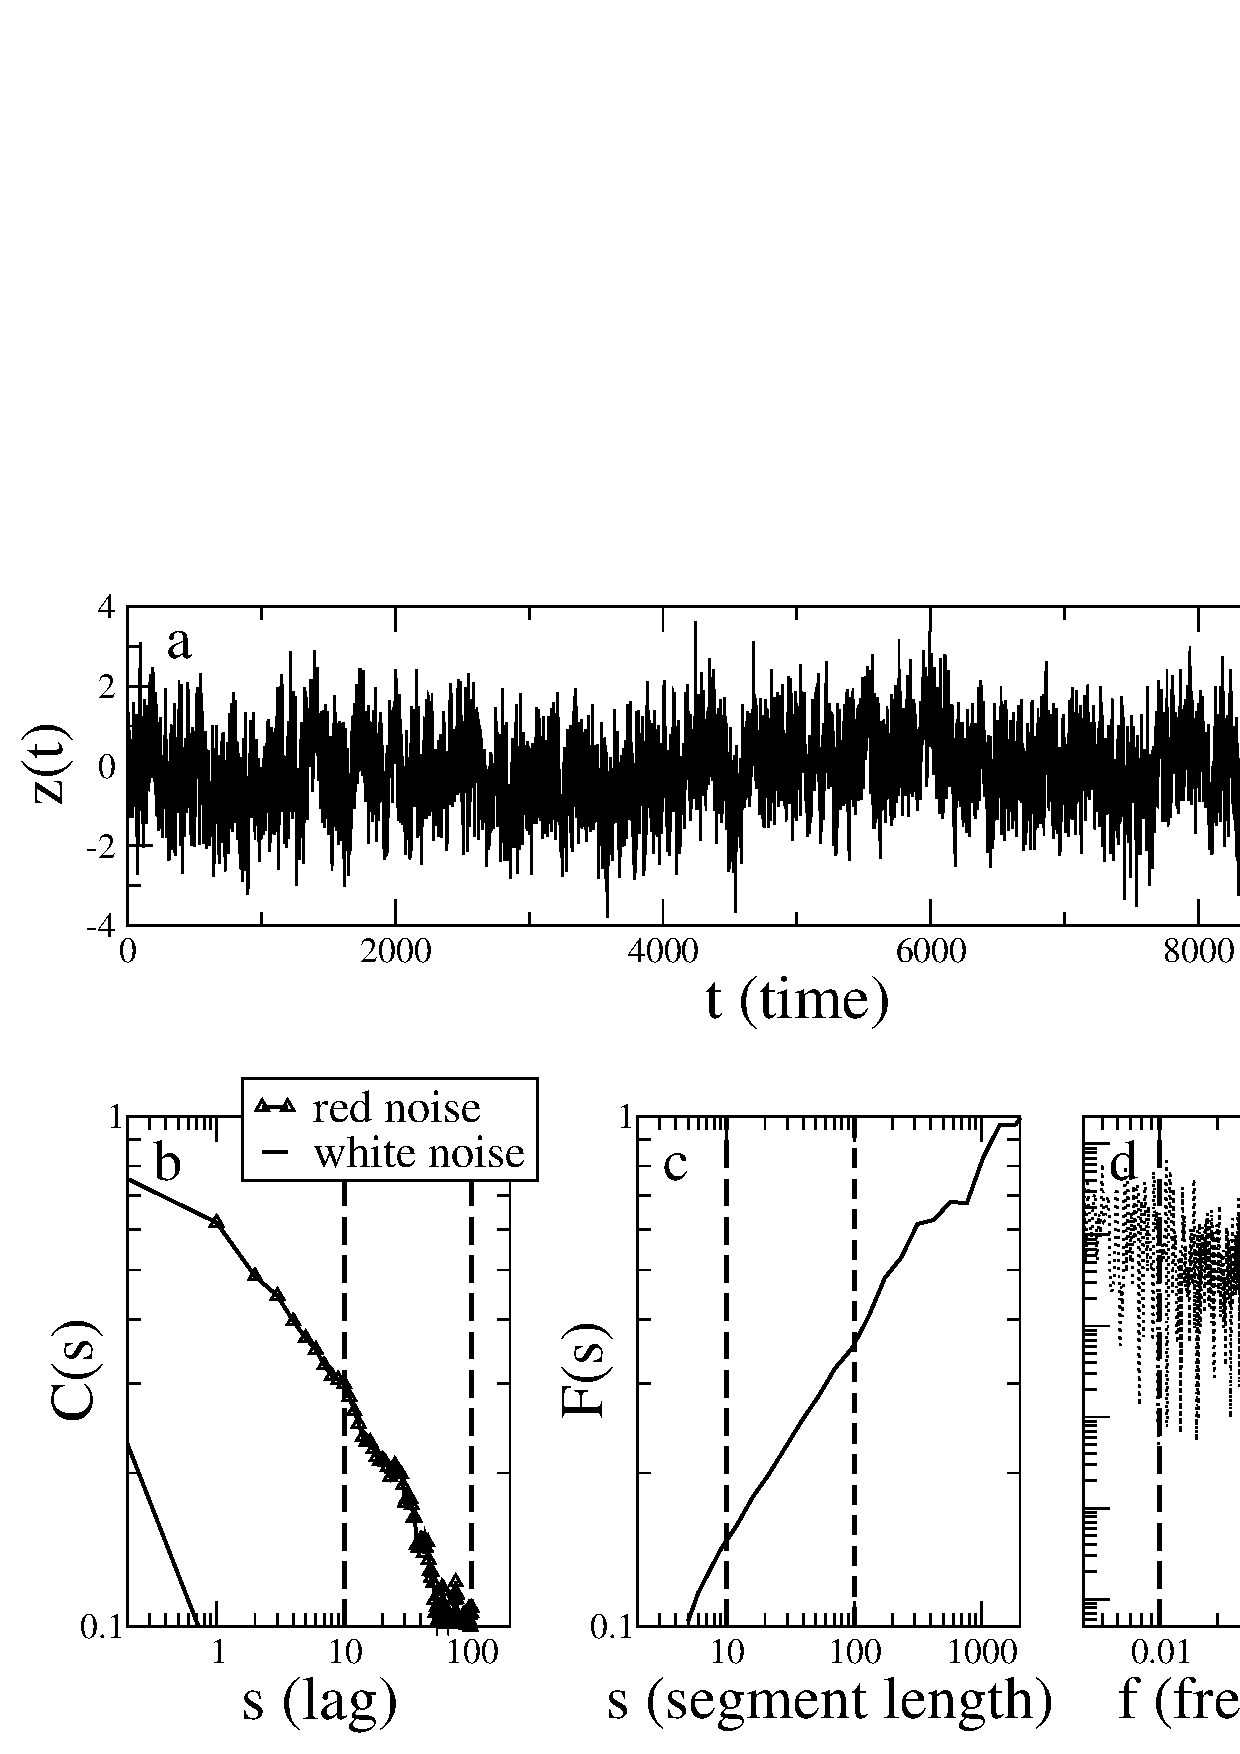
\includegraphics[width = 0.9\textwidth]{fig1_v5}
	\caption{Analysis of artificial red noise with scaling exponents measured using three different methods. Panel {\bf a}: Red noise is generated using the method shown in equation \ref{eqn:1D:simple_brownian}. Panel {\bf b}: The ACF of the red noise data is calculated for different lags and the exponent (negative slope) measured in the range $10\leq s \leq 100$ (dashed lines). We note that the ACF1 indicator ($C(1)$) is 0.84. The ACF of a white noise series is also plotted for comparison, in this case $C(s)=0$ for $s\geq 1$ and the exponent is also zero. Panel {\bf c}: DFA calculated for the data and the exponent (slope) measured in the range $10\leq s \leq 100$. Panel {\bf d}: The power spectrum of the data, and the exponent (negative slope) measured in the frequency range $10^{\m2} \leq f \leq 10^{\m1}$. \label{fig:1D:3exponents_rednoise}}
\end{figure}

\subsection{Detrended Fluctuation Analysis}
\label{subsec:1D:scaling_exponents:DFA}

Detrended Fluctuation Analysis (DFA), defined by \citet{peng1994}, is used by \citet{livina2007} as an EWS, similarly to autocorrelation. We therefore find it appropriate to draw comparisons between the two methods. Detrended Fluctuation Analysis has been applied successfully in various contexts \citep{peng1995quantification,koscielny1998,bunde2000,kantelhardt2001}. Here we describe the method used to find the DFA exponent $\alpha$.

Taking time series data $z(t)$ of length $N$, the DFA method involves calculating the cumulative sum of $z(t)$, which is called $Y$. This cumulative series is then split into $\lfloor N/s \rfloor$ non-overlapping segments $Y_{(j)},~j = 1,..., \lfloor N/s \rfloor$ and, for each segment, a `detrended' series, $\overline{Y}_{(j)}$, is found by subtracting an order-$n$ polynomial fit $p_n(Y_{(j)})$. Equations \ref{eqn:1D:DFA_method1} to \ref{eqn:1D:DFA_method2} show this process:
\begin{align}
	\label{eqn:1D:DFA_method1}
	y_i &= \sum_{k=0}^{i}x_k~~i=0,\dots,N \, ,\\
	Y_{(j)} &= \{ y_{js}, y_{js+1}, \dots, y_{(j+1)s-1}  \}~~j=0,1,\dots,\left\lfloor \frac{N}{s} \right\rfloor-1 \, ,\\
	\overline{Y}_{(j)} &= Y_{(j)} - p_n(Y_{(j)}) ~~~ j=0,1,\dots \, .
	\label{eqn:1D:DFA_method2}
\end{align}

Figure \ref{fig:1D:f2_DFAdemo} illustrates the detrending step of the DFA algorithm: the time series $z(t)$ is a pink-noise series of length 40 generated using equation \ref{eqn:1D:ColouredNoise_kasdin} with parameter $\lambda=1$ and the method shown is order-2 DFA, where a quadratic fit has been used in each segment. The detrended series $\overline{Y}$ in each segment is then the difference between $Y$ and the quadratic fit.

\begin{figure}
	\centering
	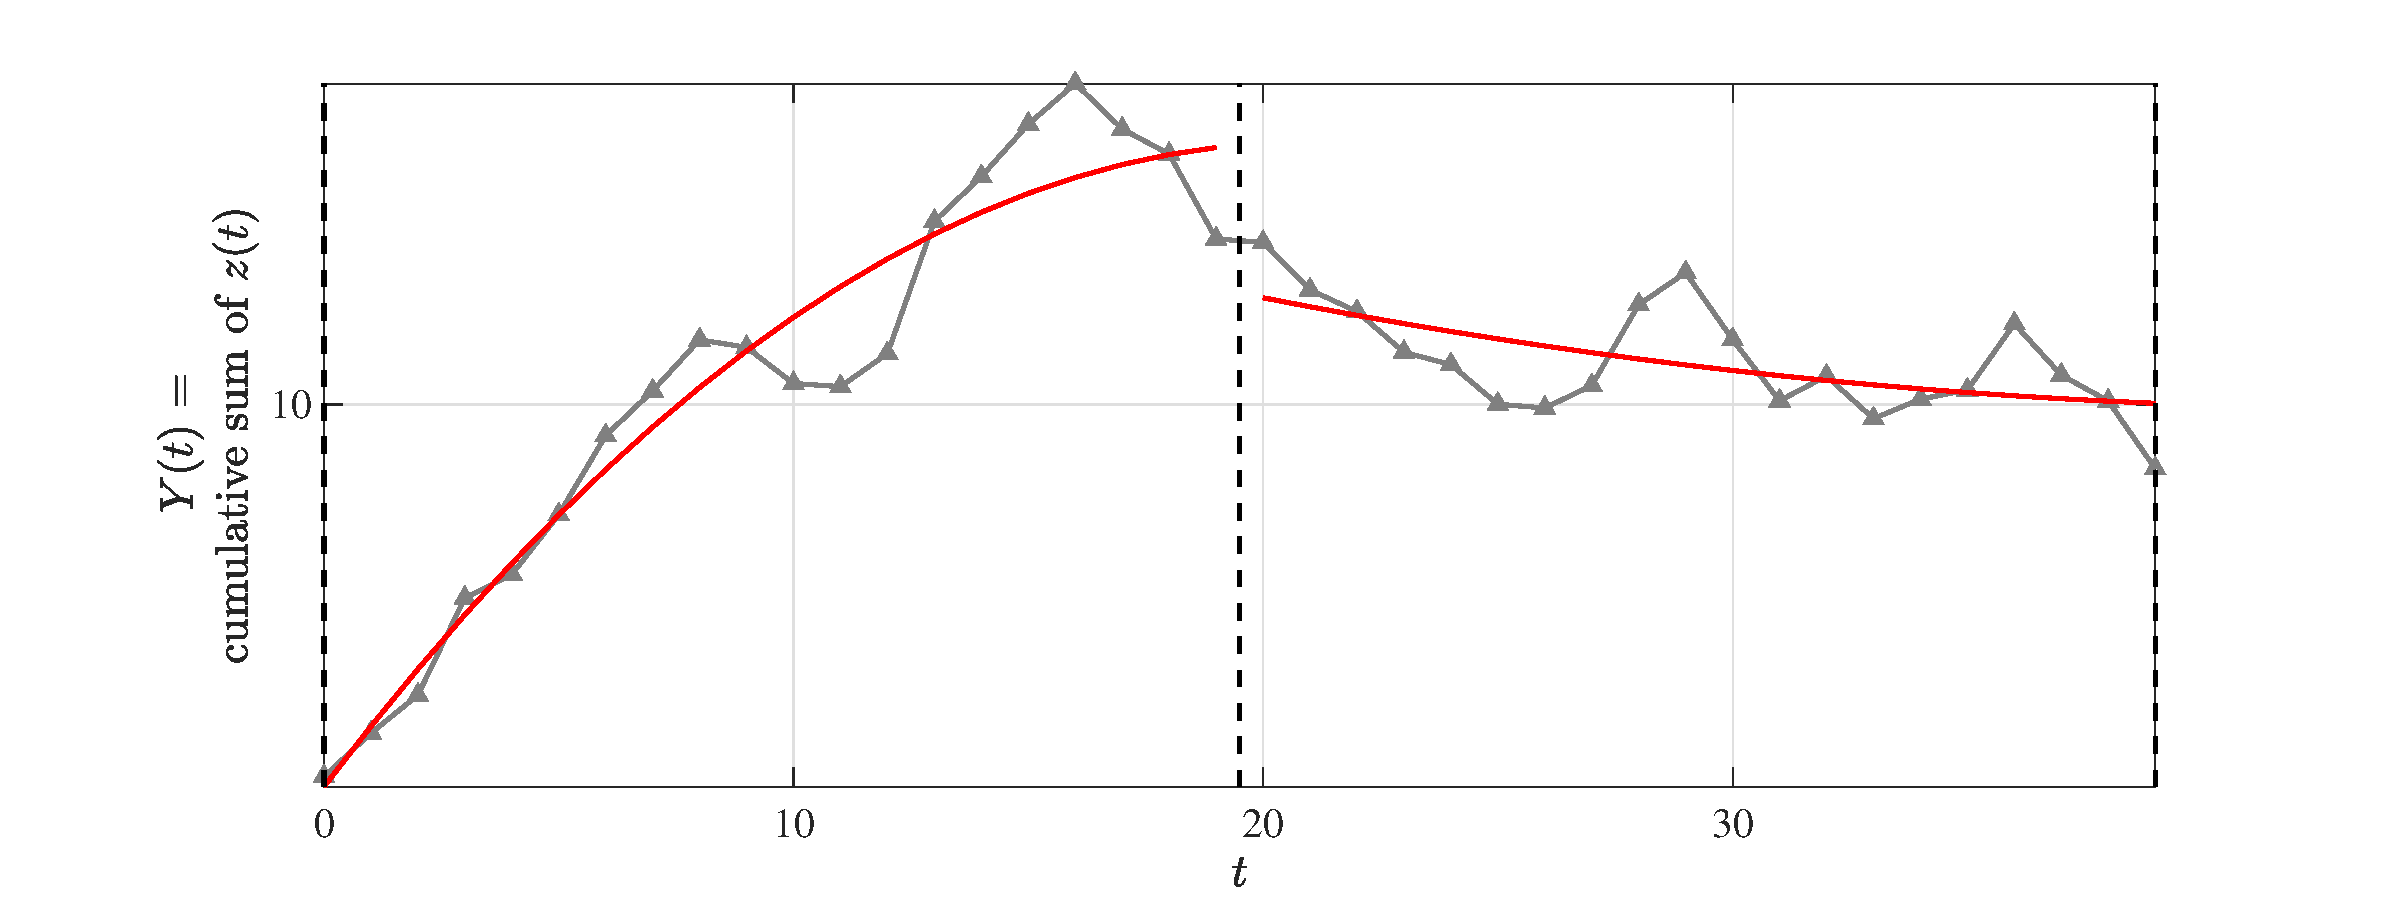
\includegraphics[width = 0.9\textwidth]{f2_DFAdemo_v2}
	\caption{The detrending step in the order-2 DFA algorithm (equation \ref{eqn:1D:DFA_method2}). The cumulative sum of a pink-noise time series $z(t)$ is shown with the quadratic best fit (red line) in each segment of length 20 (marked by dashed vertical lines). }
	\label{fig:1D:f2_DFAdemo}
\end{figure}

Given these detrended segments $\overline{Y}_{(j)}$, the equation \ref{eqn:1D:DFA} provides the $s$-dependent fluctuation coefficient $F^{(n)}(s)$:
	\begin{align}
		F^{(n)}(s) = \sqrt{ \frac{1}{\lfloor N/s \rfloor} \sum_{j=0}^{\lfloor N/s \rfloor-1} \text{Var}(\overline{Y}_{(j)})}.
		\label{eqn:1D:DFA}
	\end{align}
We define the DFA exponent in relation to the fluctuation coefficient as follows:
\begin{definition}[The DFA scaling exponent]
	\label{def:1D:DFAexponent}
	{\Red If the order-$n$ fluctuation coefficient $F^{(n)}$, as a function of segment length $s$ satisfies the power-law scaling relationship
	\begin{equation} 
		F^{(n)}(s) \sim s^{\alpha_n}, 
	\label{eqn:1D:DFA_scaling_equation} 
	\end{equation}
	then we define $\alpha_n$ as the DFA scaling exponent.}
\end{definition}
Practically, $F^{(n)}(s)$ is calculated for many values of $s$ and the value of $\alpha$ is found to be the slope of the linear best fit line to the logarithmic plot of  over $s$. Figure \ref{fig:1D:3exponents_rednoise}c shows the order-2 DFA coefficient $F^{(2)}(s)$ of the red noise time series in figure \ref{fig:1D:3exponents_rednoise}a for $s = 1,2,\dots,100$. The slope of the logarithmic plot in figure {\ref{fig:1D:3exponents_rednoise}c , obtained using a simple linear fit, is the DFA exponent $\alpha$. In this study we consistently use the order-2 DFA method, which uses a quadratic fit during the detrending step of DFA. Following the approach of \cite{livina2007}, we measure the DFA exponent in the temporal range $10\leq s \leq 100$. {\Red This range is chosen by \cite{livina2007} because, after investigation, it is found to be the range in which an increase in the DFA exponent is most sensitive to \emph{critical slowing down} which is a common feature of tipping behaviour. This is discussed further in section~\ref{subsec:1D:Exponents_as_EWS:determining_frequency_range} of this chapter where a similar investigation is carried out in the case of the power spectrum exponent.}
	
\citet{kantelhardt2001} also proposes a modified DFA method designed to provide better results with shorter time series in which long-range correlations can cause an overestimate of the exponent $\alpha$. The modified method therefore involves multiplication of the  fluctuation coefficient $F^{(n)}(s)$ by a correction function derived from $F^{(n)}(s)$ but with the segments $Y$ shuffled in a random order to destroy any long-range correlations in the data. 







\subsection{The power spectrum exponent}
\label{subsec:1D:scaling_exponents:PS}

{\Red{
Many methods of time series analysis involve transforming the series from the \emph{time domain}, in which the system state is a function of time, into the \emph{frequency domain}, in which the amount of the series lying within a frequency band is a function of frequency \citep{chatfield2016analysis}, thereby obtaining the power spectrum for the particular time series, which we define here:
}}

\begin{definition} [Power Spectrum]
	\label{def:1D:PowerSpectrum}
		{\Red{
		The Power Spectrum of a time series $x(t)$ is the Power Spectral Density (PSD) of $x(t)$ considered as a function of frequency $f$. We denote the power spectrum by $S_x(f)$. For a time series $x(t)$ with Fourier transform 
		\begin{equation}
			\label{eqn:1D:fourier_transform}
			\hat{x}(f) = \int_{\m \infty}^{\infty} x(t) e^{\m 2\pi i f t} dt,
		\end{equation}
		the power spectrum $S_x(f)$ is given by the modulus squared of the Fourier transform,
		\begin{equation}
			\label{eqn:1D:power_spectrum_def}
			S_x(f) = \left|\hat{x}(f)\right|^2\,,
		\end{equation}
		where $f\in(0,1]$ and there is symmetry about $f=1/2$. That is, $S_x(f) = S_x(1-f)$.  Alternative formulations consider the PSD as a function of angular frequency $\omega=2\pi f$.}}
\end{definition}

{\Red{
We are then able to define the power spectrum scaling exponent based on the scaling behaviour of the power spectrum as a function of frequency:
}}

\begin{definition}[The power spectrum scaling exponent]
	\label{def:1D:PSexponent}
	{\Red{If the power spectral density of a process $x(t)$, as a function of frequency $f$, satisfies the power-law scaling relationship
		\begin{equation} 
			S_x(f) \sim f^{-\beta}, 
			\label{eqn:1D:PS_scaling_relationship} 
		\end{equation}
		then we define $\beta$ as the power spectrum (PS) scaling exponent.}}
\end{definition}

{\Red{
Thus the PS scaling exponent is the negative gradient of the power spectrum $S_x(f)$ plotted on logarithmic axes, provided that the plot is linear, implying the existence of power law scaling. This view is similar to the view that the autocorrelation scaling exponent is the negative gradient of the autocorrelation $R_x$ as a function of lag $\tau$, also on logarithmic axes. 

An alternative definition of the power spectrum, or PSD, is based on the auto-correlation of the time series via the Wiener-Khinchin theorem which states that the power spectrum $S_x(f)$ is equal to the Fourier transform of the auto-correlation function \citep{chatfield2016analysis}. In this way we see that the power spectrum and the auto-correlation function are closely related, which motivates the introduction of the power spectrum scaling exponent as a tool for tipping point detection \citep{prettyman2018}. In section~\ref{sec:1D:relationships} the relationship between the DFA exponent, the ACF exponent and the power spectrum exponent is discussed further. 
}}

\begin{theorem}[The Wiener-Khinchin Theorem]
\label{thm:1D:wiener-khinchin}
	{\Red{
	For a time series $x(t)$ the auto-correlation function $R_x(\tau)$ 
	given by
	\begin{equation}
		\label{eqn:1D:W-K:auto_correlation}
		R_x(\tau) = \mathbf{E}\left[x(t)x(t+\tau)\right]
	\end{equation}
	may be expressed in terms of the power spectral density thus
	\begin{equation}
		\label{eqn:1D:wiener-khinchin1}
		R_x(\tau) = \int_{\m \infty}^{\infty} S_x(f) e^{2\pi i \tau f} df,
	\end{equation}
	which is the inverse Fourier transform \citep{chatfield2016analysis}.
	}}
\end{theorem}

{\Red{
If the terms $R$ and $S$ in equation~\ref{eqn:1D:wiener-khinchin1} satisfy the conditions of Fourier inversion, i.e. that they are absolutely integrable, then we may state the theorem as
	\begin{equation}
	\label{eqn:1D:wiener-khinchin2}
		S_x(f) = \int_{\m \infty}^{\infty} R_x(\tau) e^{\m 2\pi i \tau f} d\tau = \hat{R}_x(f).
	\end{equation}
This Fourier transform formulation is often used as the definition of the power spectrum \citep{ricker2012}, and is similarly expressed in the case of a discrete-time process $x(n)$ as follows:
	\begin{equation}
	\label{eqn:1D:wiener-khinchin:discrete}
		S_x(f) = \sum_{k=\m \infty}^{\infty} R_x(k) e^{\m 2\pi i f k},
	\end{equation}
where the discrete time autocorrelation is given by
	\begin{equation}
	\label{eqn:1D:autocorellation:discrete}
		R_x(k) = \mathbf{E}\left[x(n) x(n-k)\right].
	\end{equation}

This discrete time formulation, however, does not provide a useful method for the calculation of the power spectrum of a process given a finite time series, due to the infinite sum, even if the sample ACF is used to approximate $R_x$. Instead, in the experiments presented in this thesis, the power spectrum as defined by the Fourier transform (definition~\ref{def:1D:PowerSpectrum}) is approximated directly using the fast Fourier transform (FFT) as implemented in Matlab by \cite{frigo2005}. This straight-forward approximation of the power spectrum using a discrete-time FFT is known as a \emph{periodogram} \citep{welch1967, oppenheim1999}.
}}

\begin{definition}[Periodogram]
\label{def:1D:periodogram}
	{\Red{The periodogram $\hat{P}(f')$ of a time series $x_n$ of length $N$, as used throughout this thesis, is defined by the equation 
	\begin{equation}
		\label{eqn:1D:periodogram_def}
		\hat{P}(f') = \frac{1}{N}\left|\sum_{n=0}^{N-1}x_n e^{\m 2\pi i f' n}\right|^2, ~~~~~ f' = 0, \frac{1}{N},\frac{2}{N}, ..., 1,
	\end{equation}
	where $f'$ is a discrete variable equivalent to the frequency $f$ in the power spectrum (definition~\ref{def:1D:PowerSpectrum}). The summation term is the fast Fourier transform as implemented in Matlab \citep{frigo1998,frigo2005}. In this thesis, for the purposes of using the periodogram as a tool for tipping point detection, we consider only the one-sided periodogram, that is, the periodogram $\hat{P}(f')$ for the frequency range $f'\in (0,1/2]$, and so the calculation is performed only for the values
	\begin{equation}
		f' = \frac{1}{N},\frac{2}{N}, ..., \frac{1}{N}\left\lfloor \frac{N}{2} \right\rfloor,
	\end{equation}
	since the periodogram, as defined here, is symmetric about $f'=1/2$ \citep{fulop2006}.}}
\end{definition}


{\Red{
Having obtained the periodogram from a given discrete time series, an estimation of the power spectrum scaling exponent $\beta$ (equation~\ref{eqn:1D:PS_scaling_relationship}) is found by measuring the negative gradient of the periodogram on logarithmic axes, assuming that a power law scaling relationship exists. This is done by fitting a linear function to the logarithmic plot in a predetermined range of frequencies. When the power spectrum scaling exponent $\beta$ is estimated in this way throughout this thesis, in which $\beta$ is used as an early warning indicator, we typically use the frequency range $10^{\m2}\leq f \leq 10^{\m1}$ unless otherwise stated. This corresponds to the time scale range $10\leq s \leq 100$ used in the calculation of the DFA exponent \citep{livina2007} as discussed in section~\ref{subsec:1D:scaling_exponents:DFA} but the precise reason for this choice of frequency range is motivated by the phenomenon of \emph{critical slowing down} and will be discussed further in section~\ref{subsec:1D:Exponents_as_EWS:determining_frequency_range}. 

{\label{pageref:1D:logbinning} We note that the frequencies used in the calculation of the periodogram in equation~\ref{eqn:1D:power_spectrum_def} occur linearly between 0 and 1 and therefore the periodogram, when plotted on logarithmic axes}, has a greater concentration of points in the higher frequencies. For example, when $N=10^4$ there are 91 values of $f'$ for which $\m3\leq\log f'\leq\m2$ but 901 values of $f'$ for which $\m2\leq\log f'\leq\m1$, although both ranges are of equal length on the logarithmic scale. When a linear function is fitted to the periodogram using a least squares optimisation in order to calculate the gradient, more weight will therefore be given to the gradient described by the points at the higher end of the frequency range. In order to overcome this effect a more linear distribution of points is first obtained by binning the frequencies logarithmically, before a linear fit is attempted. The periodogram window, defined by $10^{\m2}\leq f' \leq 10^{\m1}$ (or whichever lower and upper bounds may be used), is split into a number of subwindows of equal length on the logarithmic scale such that the first subwindow contains $m$ points where $m\geq 2$. All other subwindows after the first are then divided into $m$ partitions and the new series of \emph{binned periodogram} data $P_B(f)$ is defined as the means of the periodogram points $\hat{P}(f')$ in each partition. The new series of frequencies $f$ are the midpoints (on the logarithmic scale) of the partitions. 
}}

\begin{figure}
	\centering
	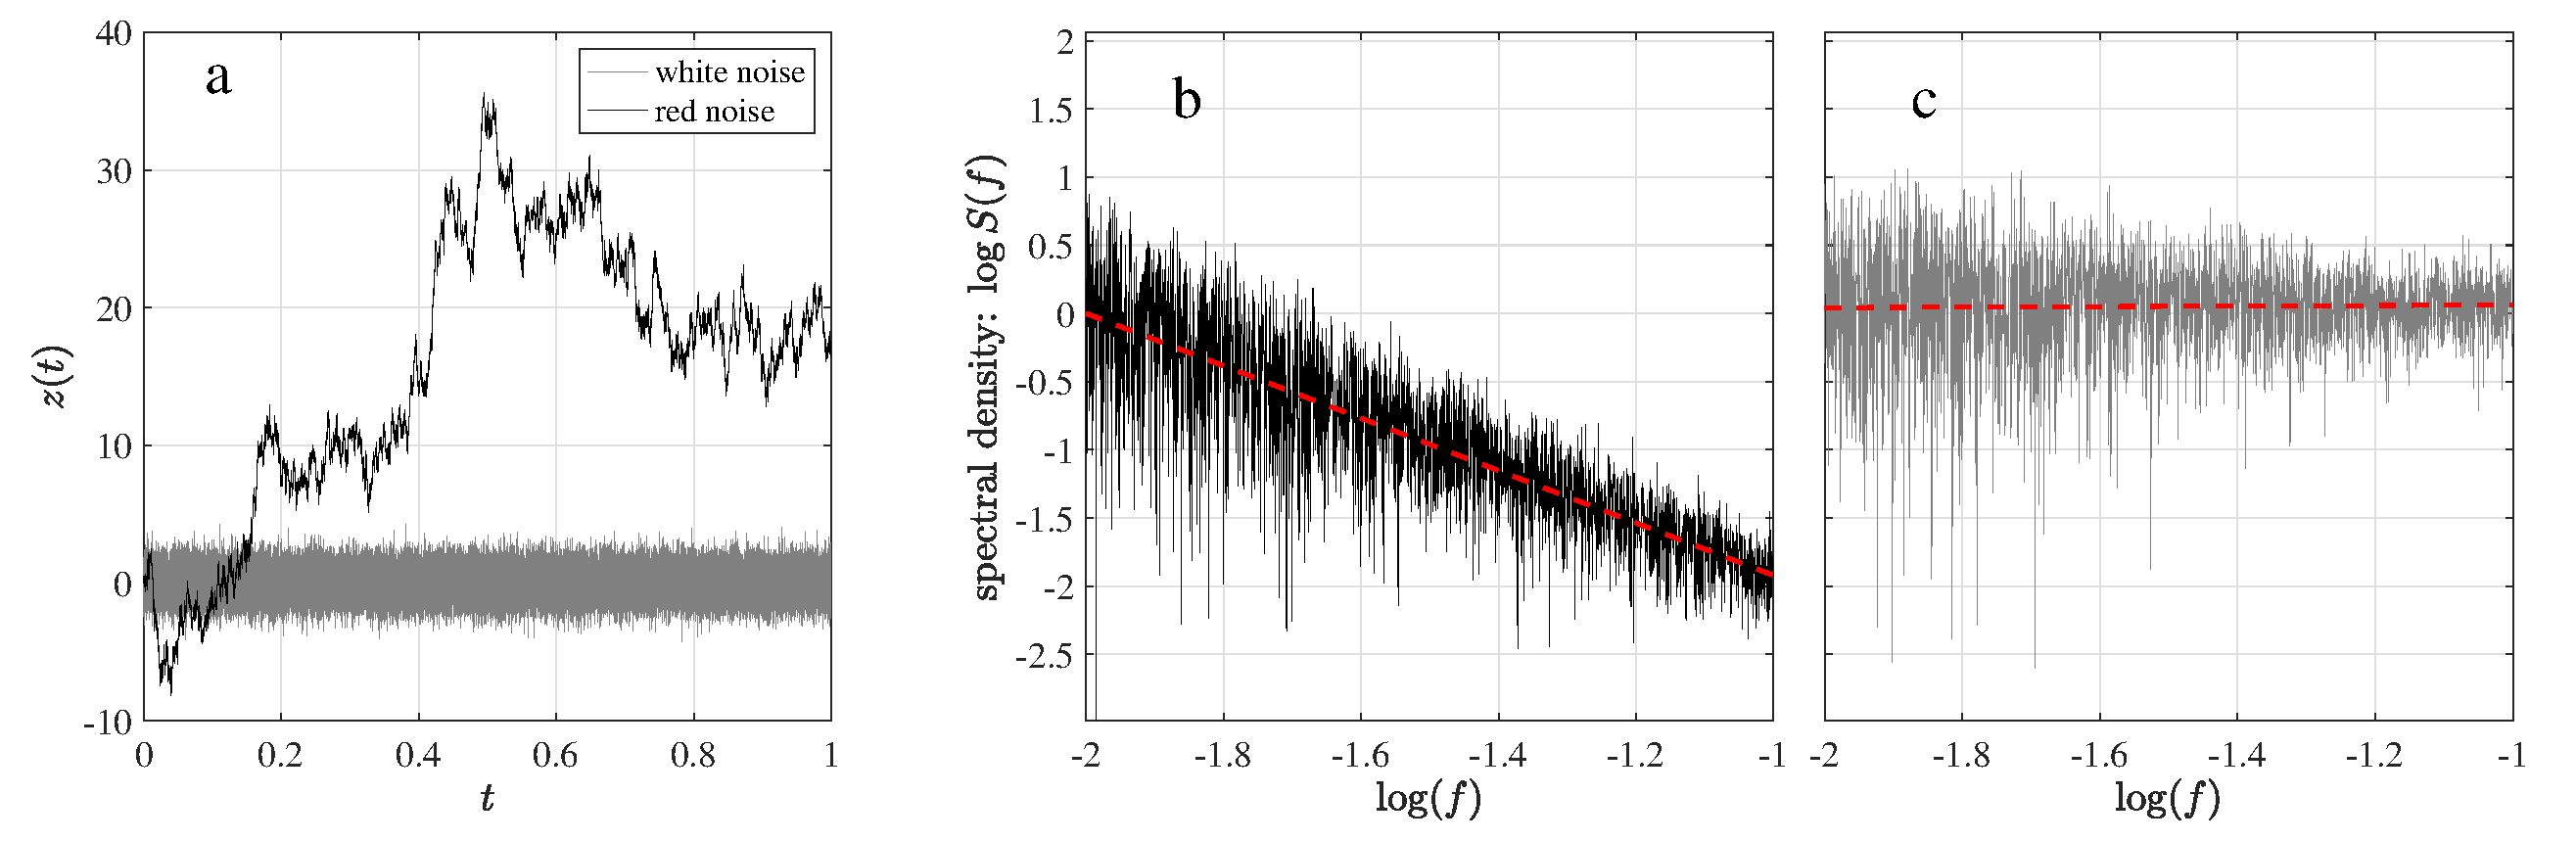
\includegraphics[width = 0.9\textwidth]{PS_scaling_calculation}
	\caption{\Red PS exponent estimation for red noise and white noise. Panel {\bf a}: A simple Gaussian discrete white noise series and a random walk (red noise, see equation~\ref{eqn:1D:simple_brownian}) are generated, both of length $10^5$. Panels {\bf b} and {\bf c}: For the red noise and white noise series respectively, the periodogram is plotted on a log-log scale in the frequency range $\m2\leq\log f\leq\m1$ and a linear best fit (dashed red line) is used to calculate the gradient. We find the PS exponents to be $1.998$ and $0.000$ for red and white noise respectively.}
	\label{fig:1D:PS_scaling_calculation}
\end{figure}

{\Red{
In figure~\ref{fig:1D:PS_scaling_calculation} the PS exponent is calculated for a red noise series and a white noise series (both of length $10^5$) using the linear best fit to estimate the negative gradient of the periodogram. In this figure the periodogram is plotted after the logarithmic binning step. By comparison, the demonstration of the same method in figure~\ref{fig:1D:3exponents_rednoise}d (page~\pageref{fig:1D:3exponents_rednoise}) does not use logarithmic binning, we note the higher variability in the higher frequencies.

Other methods exist to estimate the power spectrum, such as Welch's method \citep{welch1967} and the multi-taper method \citep{thomson1982}, both of which are based on the periodogram and are designed to reduce noise. Since, in this thesis, we are not concerned with identifying specific features of the power spectrum, only measuring the gradient to provide an estimate of the scaling exponent $\beta$, the ordinary periodogram, after logarithmic binning, is usually sufficient. If, however, it is necessary to determine whether power law scaling exists, it may be useful to reduce the noise using Welch's method in order to more easily determine visually whether power spectrum describes a straight line. Other methods of power spectrum estimation are often developed for specific applications in engineering \citep{bingham1967}.

}}



\section{Relationships between scaling exponents}
\label{sec:1D:relationships}

\subsection{White noise and red noise}
\label{subsec:1D:relationships:white_and_red_noise}
{\Red
	
In chapter~\ref{chap:intro} two examples of a noisy signal are introduced: discrete Gaussian white noise, in which each term is sampled from an independent, identical Gaussian distribution; and the discrete random walk which is the cumulative sum of Gaussian white noise. Now that we have defined the power spectrum (definition~\ref{def:1D:PowerSpectrum}) we are able to properly define the term \emph{white noise}, which is not necessarily Gaussian:

\begin{definition}[White noise]
	\label{def:1D:whitenoise}
	A white noise process $w_t$ is a random signal with equal power spectral density at all frequencies, that is, the power spectrum of the process is a constant:
	\begin{equation}
		\label{eqn:1D:white_noise_def}
		S_w(f)=\left|\hat{w}(f)\right|^2 = \left|\int_{\m \infty}^{\infty} w_t e^{\m 2\pi i f t} dt\right|^2 = C\,,
	\end{equation}
	for positive constant $C$ \citep{robinson2012introduction}.
\end{definition}

Since this power spectrum $S_w(f)$ follows the power law scaling relationship
\begin{equation}
	S_w(f) = C = f^0 C\,,
\end{equation}
we say it has PS exponent $\beta = 0$. Although we note that if a discrete time series is found to have a PS exponent of zero using the periodogram method presented in section~\ref{subsec:1D:scaling_exponents:PS}, this does not necessarily imply that the process is white noise.

A corollary of the definitions of a white noise series is that
	\begin{equation}
	\label{eqn:1D:white_noise:corollary}
		\left|\hat{w}(f)\right|^2 = C ~~\Rightarrow~~ \hat{w}(f) = \sqrt{C}e^{i\theta f}\,,
	\end{equation}
for some $\theta\in [\m\pi, \pi]$. In this thesis only Gaussian white noise is considered, in which case the distribution of the values of $w_t$ will be Gaussian, although many other distributions of values could also result in a constant power spectrum. In computational examples and experiments throughout this thesis, whenever a white noise series is required, a discrete-time series of length $N$ is generated simply by using the Matlab random number generator function $\texttt{randn(1,N)}$, which returns $N$ independent identically distributed values sampled from a normal distribution with mean zero and variance $\sigma^2=1$. 

We are then able to show that the Gaussian noise process $\eta_t$, as we have been using it, actually is a white noise process according to the definition. From the simple observation that the expected value of the product of two independent random variables with zero mean is zero, we can express the autocorrelation function of the Gaussian white noise as
\begin{equation}
	\label{eqn:1D:white_noise:autocorellation}
	R_\eta(k) = \mathbf{E}\left[\eta(n) \eta(n-k)\right] 
	= \left\{ \begin{array}{lr}
	0 , & k\neq 0 \\
	1 , & k=0
	\end{array} \right. ,
\end{equation}
where, in this case, the variance of the white noise terms $\eta$ is 1. This result is similar in appearance to the continuous-time case which can be derived from the Wiener-Khinchin theorem. The theorem defines the autocorrelation $R_x$ of process $x$ as the inverse Fourier transform of the power spectrum. Since the power spectrum of white noise is a constant, we have
\begin{equation}
	\label{eqn:1D:autocorrrelation_dirac}
	R_eta(\tau) = \int_{\m \infty}^\infty S_\eta(f)e^{2\pi i \tau f}df = C\int_{\m \infty}^\infty e^{2\pi i \tau f}df = C\delta(\tau)\,,
\end{equation} 
since the inverse Fourier transform of the constant function $S(f)=1$ is the Dirac delta function \citep{kammler2007fourier} which has an infinitely large spike at $\tau =0$. We note that, clearly, there does not exist power law scaling for the function $R_\eta$. The discrete-time formulation in equation~\ref{eqn:1D:white_noise:autocorellation} allows us, using the discrete-time Wiener-Khinchin theorem (equation~\ref{eqn:1D:wiener-khinchin:discrete}), to calculate the power spectrum as follows:
\begin{equation}
\label{eqn:1D:PSofWhiteNoise}
	S_\eta(f) = \sum_{k=\m \infty}^{\infty} R_\eta(k) e^{\m 2\pi i f k} = R_\eta(0) e^{0} = 1\,.
\end{equation}
The power spectrum of the Gaussian noise is thus constant and is therefore white noise according to definition~\ref{def:1D:whitenoise}. We are also able to compute the power spectrum of the random walk series, simply the cumulative sum of a Gaussian white noise series. This is the discrete time analogue of the continuous Wiener process, which is defined as a process $W_t$ such that the derivative is a Gaussian process:
\begin{equation}
	\label{eqn:1D:Wiener_process}
	\frac{d}{dt}W_t = \eta_t.
\end{equation}
Or, conversely, as the integral of a Gaussian process. Using this definition we may compute the power spectrum of a Wiener process using the Fourier transform identity that if $\hat{x}(f)$ is the Fourier transform of $x(t)$, then 
\begin{equation}
	\widehat{\frac{d}{dt}x(t)} = (2\pi i f)\hat{x}(f).
\end{equation} 
For the Wiener process this identity becomes
\begin{equation}
	\widehat{\frac{d}{dt}W_t} = (2\pi i f)\hat{W}_t\,,
\end{equation} 
or
\begin{equation}
	(2\pi i f)\hat{W}_t = \hat{\eta}_t = e^{i\theta f}\,,
\end{equation} 
for some $f\in[\m\pi, \pi]$, as shown in equation~\ref{eqn:1D:white_noise:corollary}. Therefore the power spectrum is given by
\begin{equation}
	\label{eqn:1D:rednoise_scalingfactor}
	S_W(f) = \left|\hat{W}_t\right|^2 = \left|\frac{e^{i\theta f}}{2\pi i f}\right|^2 = \frac{1}{4\pi^2}f^{\m 2}\,,
\end{equation} 
and so the Wiener process has power spectrum scaling exponent $\beta = 2$. While a stochastic process with a constant power spectrum is known as \emph{white noise}, and this has PS exponent $\beta =0$, the random walk, or Wiener process, with a PS scaling exponent of $\beta = 2$ is known as \emph{red noise}. Stochastic processes with PS scaling exponent in the range $0<\beta<2$ are known as \emph{pink noise} (given that a power law scaling relationship exists). It is often a ``reddening'' of noise, the increase in the PS exponent from 0 to 2, that we will try to detect when investigating tipping points. Recalling the changing shape of the generalised potential ``well'' in the pitchfork bifurcation example (see figure~\ref{fig:intro:ChangingPotential}, page~\pageref{fig:intro:ChangingPotential}), we are able to understand intuitively why such reddening of noise, a building up of memory in the system, may occur. When the the generalised potential is a steep ``well'' shape we expect that any small perturbation from the stable state will return quickly to the mean. However, as the shape becomes shallower, small perturbations may continue in the direction away from the mean, resembling a random walk. This increased return time to the stable state is known as \emph{critical slowing down} \cite{scheffer2009critical} and is a typical feature of tipping points in dynamical systems, not only the pitchfork bifurcation. 

}

\subsubsection{The relationship between $\beta$ and $\gamma$}
\label{subsec:1D:relationships:beta_and_gamma}
{\Red
	
The Wiener-Khinchin theorem (theorem~\ref{thm:1D:wiener-khinchin}) states that there is a relationship between the autocorrelation $R_x$ and the power spectrum $S_x$ of a process $x$ in that the two are a Fourier transform pair, that is
	\begin{equation}
		R_x(\tau) = \int_{\m \infty}^\infty S_x(f)e^{2\pi i \tau f} df\,.
	\end{equation}
Indeed, this relation is often used to define the power spectrum \citep{chatfield2016analysis}. We now use this theorem to investigate the relationship between the ACF scaling exponent $\gamma$ and the PS scaling exponent $\beta$. Say the process $x$ has a power spectrum scaling exponent $\beta$, then by definition we have $S_x(cf) = c^{\m\beta}S_x(f)$
for some constant $c$, or
	\begin{equation}
		S_x(f) = c^{\beta}S_x(cf)\,.
	\end{equation}
Now we attempt to find if power law scaling exists for the autocorrelation function by calculating $R_x(c\tau)$ as follows:
	\begin{equation}
	\begin{split}
		R_x(c\tau) &= \int_{\m \infty}^\infty S_x(f)e^{2\pi i c\tau f} df\\
		&= \int_{\m \infty}^\infty c^{\beta}S_x(cf)e^{2\pi i c\tau f} df\,.
	\end{split}
	\end{equation}
Using the substitution $g = cf$, and so $df/dg = 1/c$, we obtain
	\begin{equation}
	\begin{split}
	R_x(c\tau) &= \int_{\m \infty}^\infty c^{\beta}S_x(g)e^{2\pi i \tau g} \frac{1}{c} dg\\
	&= c^{\beta\m 1}\int_{\m \infty}^\infty S_x(g)e^{2\pi i \tau g} dg\\
	&= c^{\m(1\m\beta)}R_x(\tau)\,.
	\end{split}
	\end{equation}
Then we see that the process $x$ has an ACF scaling exponent $\gamma = 1-\beta$, thus giving a relationship between the PS and ACF exponents:
	\begin{equation}
	\label{eqn:1D:beta-gamma_linear_relation}
		\beta = 1-\gamma\,,
	\end{equation}
where scaling exists in both the ACF and the power spectrum. As we have noted above (equation~\ref{eqn:1D:autocorrrelation_dirac}) there is not strictly power law scaling in the autocorrelation function of white noise, even though there is scaling in the power spectrum. The autocorrelation of the ``red noise'' Wiener process would be given by the Wiener-Khinchin theorem as
	\begin{equation}
		\begin{split}
		R_W(\tau) &= \int_{\m \infty}^\infty S_W(f)e^{2\pi i \tau f} df\,,\\
		&= \int_{\m \infty}^\infty \frac{1}{|2\pi f|^2}e^{2\pi i \tau f} df\,,
		\end{split}
	\end{equation}
but it is not possible to evaluate the integral because of the singularity at $f=0$ \citep{kammler2007fourier}. Taking a different approach, we look to the definition of the \emph{normalised} autocorrelation
	\begin{equation}
		R_{W_t}(\tau) = \frac{1}{\sigma_{W_t} \sigma_{W_{t+\tau}}} \mathbf{E}\left[W_t W_{t+\tau}\right].
	\end{equation}
where $\sigma_{W_t}^2$ is the variance of the Wiener process $W$ at time $t$. The properties of the Wiener process lead to the expression
	\begin{equation}
		R_{W_t}(\tau) = \sqrt{\frac{t}{t+\tau}}, 
	\end{equation}
\citep{stark2002probability} where the dependence on $t$ comes from the fact that the Wiener process is non-stationary. Clearly, for some fixed value $t$, this is not a power-law scaling relationship in $R_{W_t}$ as a function of $\tau$. 

We have shown here that $\beta$ and $\gamma$ are related linearly as $\beta = 1-\gamma$, and also that in the case of a white noise process and also the Wiener process, the autocorrelation function does not exhibit power-law scaling and so $\gamma$ does not exist. Table~\ref{tab:1D:exponent_relationships} shows the results of attempting to numerically estimate the scaling exponents given a finite, discrete time series. Two processes are used to generate the time series: a Gaussian white noise process where each term is sampled independently from a Gaussian distribution; and a random walk which is simply the cumulative sum of a Gaussian white noise series. The scaling exponents are estimated using the methods described in section~\ref{sec:1D:scaling_exponents}, where the range of lags in which $\gamma$ is estimated by linear fit is $10\leq\tau\leq100$ and the range of frequencies in which $\beta$ is estimated is $10^{\m2}\leq f \leq 10^{\m1}$. In this case the range is arbitrary since, if power law scaling exists, then it does not matter in which range the exponent is measured because the (logarithmic) power spectrum is a straight line over the whole domain $0\leq f \leq 1/2$. However, in other contexts the range does have a significant impact on the method: the reasons why this particular range $10^{\m2}\leq f \leq 10^{\m1}$ is used consistently throughout this thesis will be discussed in section~\ref{subsec:1D:Exponents_as_EWS:determining_frequency_range}. The values of $\alpha$, $\beta$, $\gamma$ and the lag-1 ACF presented in table~\ref{tab:1D:exponent_relationships} are the mean values over 1000 trials of the experiment using, in each experiment, a Gaussian white noise time series and a random walk time series of length $10^6$.

We note that the PS exponent behaves as predicted with a value $\beta=0$ (constant power spectrum) for white noise and $\beta=2$ (power spectrum scales as $f^{\m 2}$) for the random walk. However, the linear relation with the ACF exponent, $\gamma = 1-\beta$, which is shown to exist based on the definitions, does not hold. This is because the relationship is shown to exist only when power-law scaling is assumed to exist in both the power spectrum and the ACF and, as we have shown, the ACF does not exhibit power-law scaling for Gaussian white noise nor the random walk. We are able to note that the value in the case of white noise, $\gamma=0$, is expected from the analytical calculations, so long as the range of lags in which the exponent is estimated does not include $\tau=0$ (which is where the delta function spike occurs). Since the ACF for the random walk is a function of $\tau$ which is not a power law, it describes a curve, rather than a straight line, in the logarithmic plot and the local gradient will depend on the range of lags used. In section~\ref{subsec:1D:Exponents_as_EWS:nopowerlawsacaling} we will discuss the relevance of estimating scaling exponents in series for which power-law scaling does not exist. 

}

\subsubsection{The relationship between $\alpha$ and $\beta$}
\label{subsec:1D:relationships:alpha_and_beta}
\begin{table}
	\centering
	\begin{tabular}{l  r r r r }
		\toprule
		& \multicolumn{4}{c}{Exponent} \\
		\cmidrule(r){2-5}
		Signal    & DFA ($\alpha$) & PS ($\beta$) & ACF ($\gamma$) & lag-1 ACF  \\
		\midrule
		{White Noise} & 0.510 & 0.0110&-0.0163 & -0.00371 \\
		{Random Walk}   & 1.50  & 2.04 & 0.473  &  0.993\\
		%{Red 63}& 1.48 & 1.92 & 0.565  &  0.990\\
		\bottomrule
	\end{tabular}
	\caption{Mean values of three scaling indicators, and lag-1 ACF, applied to different noise signals.
	\label{tab:1D:exponent_relationships}}
\end{table}

The three scaling exponents defined in section \ref{sec:1D:scaling_exponents} are illustrated in figure \ref{fig:1D:3exponents_rednoise} where they are applied to a red noise series. The red noise, in this case, is a random walk, the simple cumulative sum of a white noise series (see equation~\ref{eqn:1D:simple_brownian}). Since all three methods give a measure of scaling, there is a relationship between them. 

Table \ref{tab:1D:exponent_relationships} shows the results of calculating the value of each exponent for both a white noise series and a random walk. In each case the value given is the mean value of the exponent calculated for $1000$ series of length $10^6$.
   
The values of $\alpha$ and $\beta$ in table \ref{tab:1D:exponent_relationships} confirm the linear relationship
	\begin{equation} 
		\alpha = \frac{1+\beta}{2} \label{eqn:1D:alphabetaExponentRelationships} 
	\end{equation}
noted by \citet{kantelhardt2001} to apply generally to these exponents. We have shown already (equation~\ref{eqn:1D:beta-gamma_linear_relation}) that the ACF scaling exponent $\gamma$ is also linearly related to $\beta$ as $\beta=1-\gamma$ where $\gamma$ and $\beta$ exist (that is, where a power law scaling relation exists for the ACF and the power spectrum). All three exponents therefore have the relationship
	\begin{equation}
		\beta = 2\alpha-1 = 1-\gamma\,,
	\end{equation} 
as noted by \cite{makse1996}. The relationship between $\alpha$ and $\beta$ is also noted by \citet{heneghan2000} to exist only for long-range correlated noise series, although here we have used only uncorrelated white noise and the random walk as a single example of a correlated series. In a further experiment, the DFA and PS exponents are calculated for multiple noise series with spectral densities between white and red noise. In this experiment we use two alternate methods of generating a noise series. The first method is the an auto-regressive model of order 1, or AR(1) model, given by the equation 
	\begin{equation}
		z_{n} = \mu z_{n-1}+\eta_{n}
	\label{eqn:1D:AR1_model}
	\end{equation}
where $\eta$ is white noise. This noise signal we refer to as being "short-range correlated", since the correlation is defined by parametrising the lag-1 autocorrelation by the single parameter $\mu$. We use $\mu=0, 0.005, \dots, 1$ to generate 200 short-range correlated noise series of length $10^6$ using this AR(1) model. 

The second method of generating a noise signal, which we call "long-range correlated", is to use an AR(63) model, described by \citet{kasdin1995}, since this is implemented in Matlab's DSP system toolbox. Simply, the method uses an auto-regressive model of order 63 with a zero-mean white noise signal $\eta(t)$:
	\begin{equation}
		\sum_{i=0}^{63} a_i z(t-i) = \eta(t),
	\label{eqn:1D:ColouredNoise_kasdin}
	\end{equation}
where the AR coefficients $a_i$ are calculated recursively by
	\begin{equation}
		a_0 = 1 ~~~~ a_k = \left(k-1-\frac{\lambda}{2}\right)\frac{a_{k-1}}{k} ~~~ k=1,2,\dots\, .
	\end{equation}
We note that where $\lambda=2$ the coefficients are 
	\begin{equation}
		a_0 = 1 ~,~ a_1 = -1 ~,~~ a_i = 0 ~~\forall i\geq2\,,
	\end{equation}
which results in the same process as defined by the AR(1) model for $\mu=1$, that is, a random walk. {\Red However, for other values of the parameter $\lambda$ the two methods differ. A value $\lambda=1$ does not correspond, for example, to the AR(1) process with $\mu=1/2$, in the former case parameters are given by
	\begin{equation}
		a_0 = 1 ~,~ a_1 = -\frac{1}{2} ~,~ a_2 = -\frac{1}{8} ~,~ a_3 = \frac{\m 1}{16}~,~ a_4 = \frac{\m 5}{128}~,~\dots\,,
	\end{equation}
giving us the AR(63) process
	\begin{equation}
		z_{t+1} = \frac{1}{2}z_{t} + \frac{1}{8}z_{t-1} + \frac{1}{16}z_{t-2} + \frac{5}{128}z_{t-3} + \dots + \eta_{t+1}\,,
	\end{equation}
as opposed to the AR(1) process
	\begin{equation}
		z_{t+1} = \frac{1}{2}z_{t} + \eta_{t+1}\,.
	\end{equation}
The additional coefficients $a_2$, $a_3$, etc., not present in the AR(1) model, introduce additional long-range correlations into the process. }
For the experiment we generate 200 series by this method, with a range of $\lambda$ between $0$ and $2$.

\begin{figure}
	\centering
	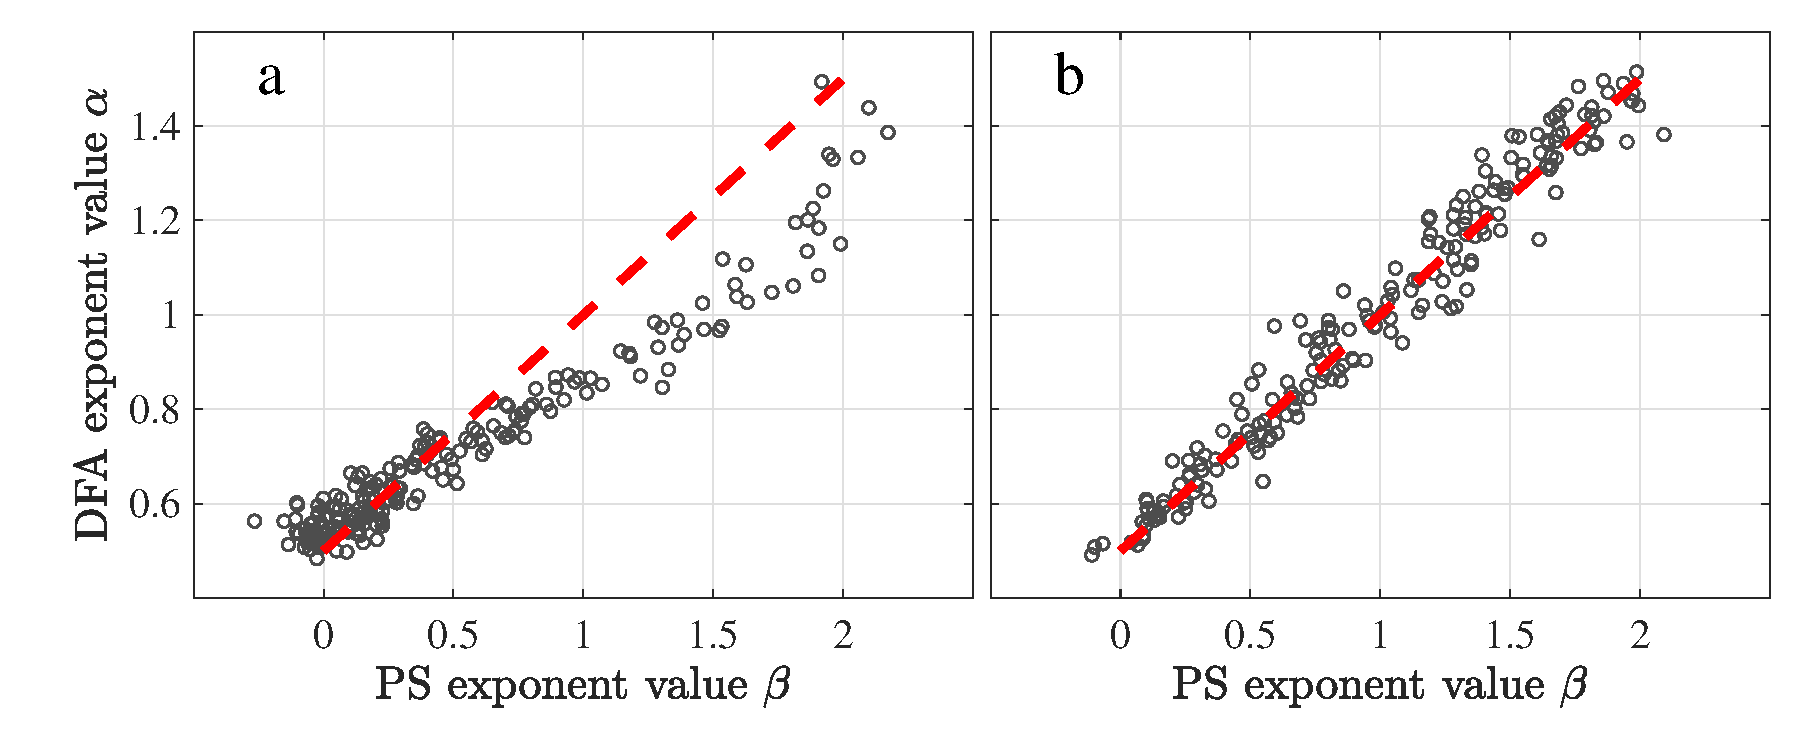
\includegraphics[width=0.9\textwidth]{f3_ExponentRelationships_v2}
	\caption{DFA exponent $\alpha$ plotted against the PS exponent $\beta$ for short-range correlated (panel {\bf a}) and long-range correlated (panel {\bf b}) noise series of length $10^4$ with varying correlation parameters. The result for each noise series is represented by one marker, the expected linear relationship is shown in red, see equation \ref{eqn:1D:alphabetaExponentRelationships}.}
	\label{fig:1D:ExponentRelationships}
\end{figure}

The DFA and PS exponents are calculated for each of the 200 short-range correlated (AR(1)) series and each of the 200 long-range correlated (AR(63)) series. The results are shown in figure \ref{fig:1D:ExponentRelationships}. We see that although the linear relationship given by equation \ref{eqn:1D:alphabetaExponentRelationships} is confirmed by the long-range correlated noise (panel {\bf b}), but not exactly by the short-range (panel {\bf a}).

An alternative method of producing long range correlated noise was to transform the power spectrum of white noise in the frequency domain, thus changing the PS exponent $\beta$ \citep{makse1996}. That is, we first sample from a Gaussian distribution to approximate white noise, $X(t)$, we then take the fast Fourier transform of this white noise series (denoted $\hat{X}(f)$) and then transform this by
	\begin{equation} 
	\label{eqn:1D:creatingColouredNoise}
		\hat{Y}(f) := \hat{X}(f)\sqrt{f^{-\beta}}.
	\end{equation}
Finally, we use the inverse fast Fourier transform to obtain the series $Y(t)$ in the time domain, which has power spectrum $S(f)$ proportional to $f^{-\beta}$. The result when using this method of noise generation is quantitatively and qualitatively similar to the result when using the AR(63) model (figure \ref{fig:1D:ExponentRelationships} panel {\bf b}): the DFA and PS exponents are strongly correlated and obey the linear relationship $\alpha = (1+\beta)/2$.


\citet{kantelhardt2001} notes that a direct calculation of the ACF scaling exponent $\gamma$ is often unsuitable due to noise and underlying trends. The DFA method is therefore introduced as an indirect measure of the exponent. In our own implementations of the two methods, the ACF exponent is less reliable. Figure \ref{fig:1D:ACFDFAreliability} illustrates this in the case that both methods are applied to noise series generated using the AR(63) model \citep{kasdin1995} with varying values of the parameter $\lambda$. Fifty noise series of length $10^4$ are generated for each value $\lambda = 0, 0.02, 0.04, ..., 1$, at each value $\lambda$ the scaling exponent is calculated for each of the 50 series and the standard deviation over these 50 exponents is found. We see that the DFA exponent is consistent in that the standard deviation of its value is low, and indeed the standard deviation is, itself, consistently low. The standard deviation is much larger in the ACF exponent, although the exponents have similar mean values (between 0 and 1).





\begin{figure}
	\centering
	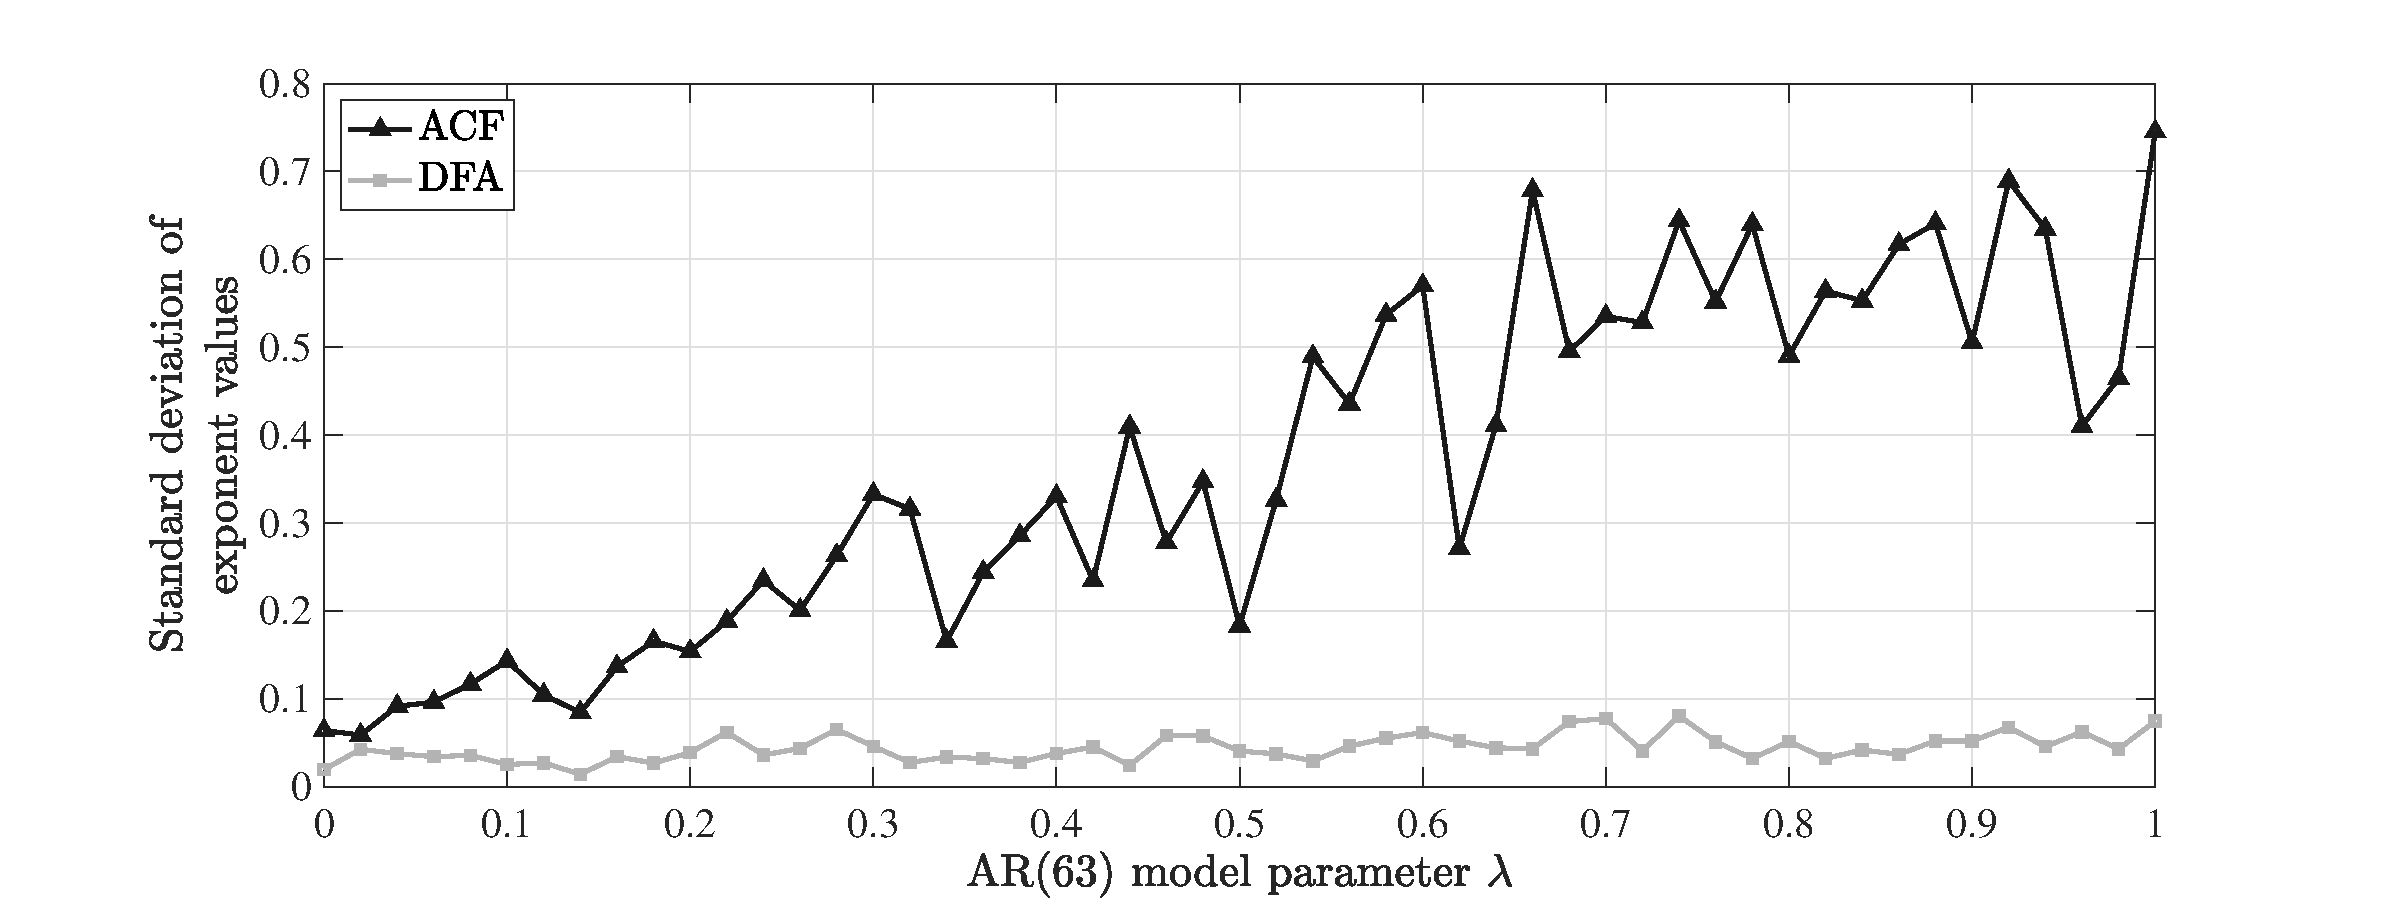
\includegraphics[width = 0.9\textwidth]{f4_ACF_DFA_reliability_v2}
	\caption{Standard deviation of the ACF and DFA scaling exponents over 50 noise series of length 1000, for each noise correlation parameter $\lambda = 0, 0.02, 0.04, ..., 1$. The mean values of the exponents range between 0 and 1.2 (ACF), and between 0.5 and 1 (for DFA).}
	\label{fig:1D:ACFDFAreliability}
\end{figure}
 

\subsubsection{The relationship between $\gamma$ and the lag-1 autocorrelation}

We also investigate the relationship between the ACF scaling exponent and the simple lag-1 autocorrelation function (ACF1). While the ACF exponent is unreliable and the superior DFA exponent has been introduced specifically as a more reliable measure \citep{kantelhardt2001}, the ACF1 has been widely used in tipping-point research \citep{held2004,dakos2008} and is much less computationally expensive than the calculation of the scaling exponents detailed in this chapter. 

Figure \ref{fig:1D:ACFrelationships} shows the ACF scaling exponent and the ACF1 calculated for 200 short-range correlated noise series (panel {\bf a}), and 200 long-range correlated noise series (panel {\bf b}), with varying correlation parameters. The short-range correlated noise is produced using an AR(1) model (equation \ref{eqn:1D:AR1_model}) and the long-range correlated noise is produced using the AR(63) model \citep{kasdin1995}.

We note that the lag-1 ACF is an estimator of the AR(1) model parameter $\lambda$ and we would expect the two values to be approximately equal, which is evident in figure \ref{fig:1D:ACFrelationships} panel {\bf a}. The ACF scaling exponent, however, does not respond to any increase in the parameter below the value of $\lambda= 0.7$, although it does increase with increasing $\lambda$ for larger values when the noise can be said to be "red". For low values of $\lambda$ the autocorrelation functions with lag $\geq2$ are approximately zero and so the ACF decays exponentially after lag-1 making it essentially useless. The behaviour is similar in the DFA and PS exponents, we now note the cluster of points in figure \ref{fig:1D:ExponentRelationships} panel {\bf b} for low exponent values, because a measure of scaling is not suitable for this particular short-range correlation. We note also that the ACF exponent displays large variability for $\lambda>0.7$, as already noted for long-range correlated noise (see figure \ref{fig:1D:3exponents_rednoise}). 

In figure \ref{fig:1D:ACFrelationships} panel {\bf b} we see that the lag-1 ACF increases linearly with the AR(63) model parameter $\lambda$ until $\lambda=1$ (red noise) after which it tends to its maximum value 1. The ACF scaling exponent also increases, apparently linearly, with $\lambda$, until $\lambda\approx0.7$ after which it decreases to zero. In the case of the AR(1) model with $\lambda<0.7$ the ACF exponent is zero because the ACF for all lags in the range $[10, 100]$ is zero and so the linear fit to the points in this range has a slope of zero. In contrast, the AR(63) model with $\lambda=2$ also has an ACF exponent close to zero but because the ACF for all lags in the range $[10, 100]$ is close to 1. Over 1000 noise series were produced using the same AR(63) model, with $\lambda=2$, in order to evidence the phenomenon. The lag-10 ACF had a mean value of 0.98 and the lag-100 ACF had a mean value of 0.83. 


\begin{figure}
	\centering
	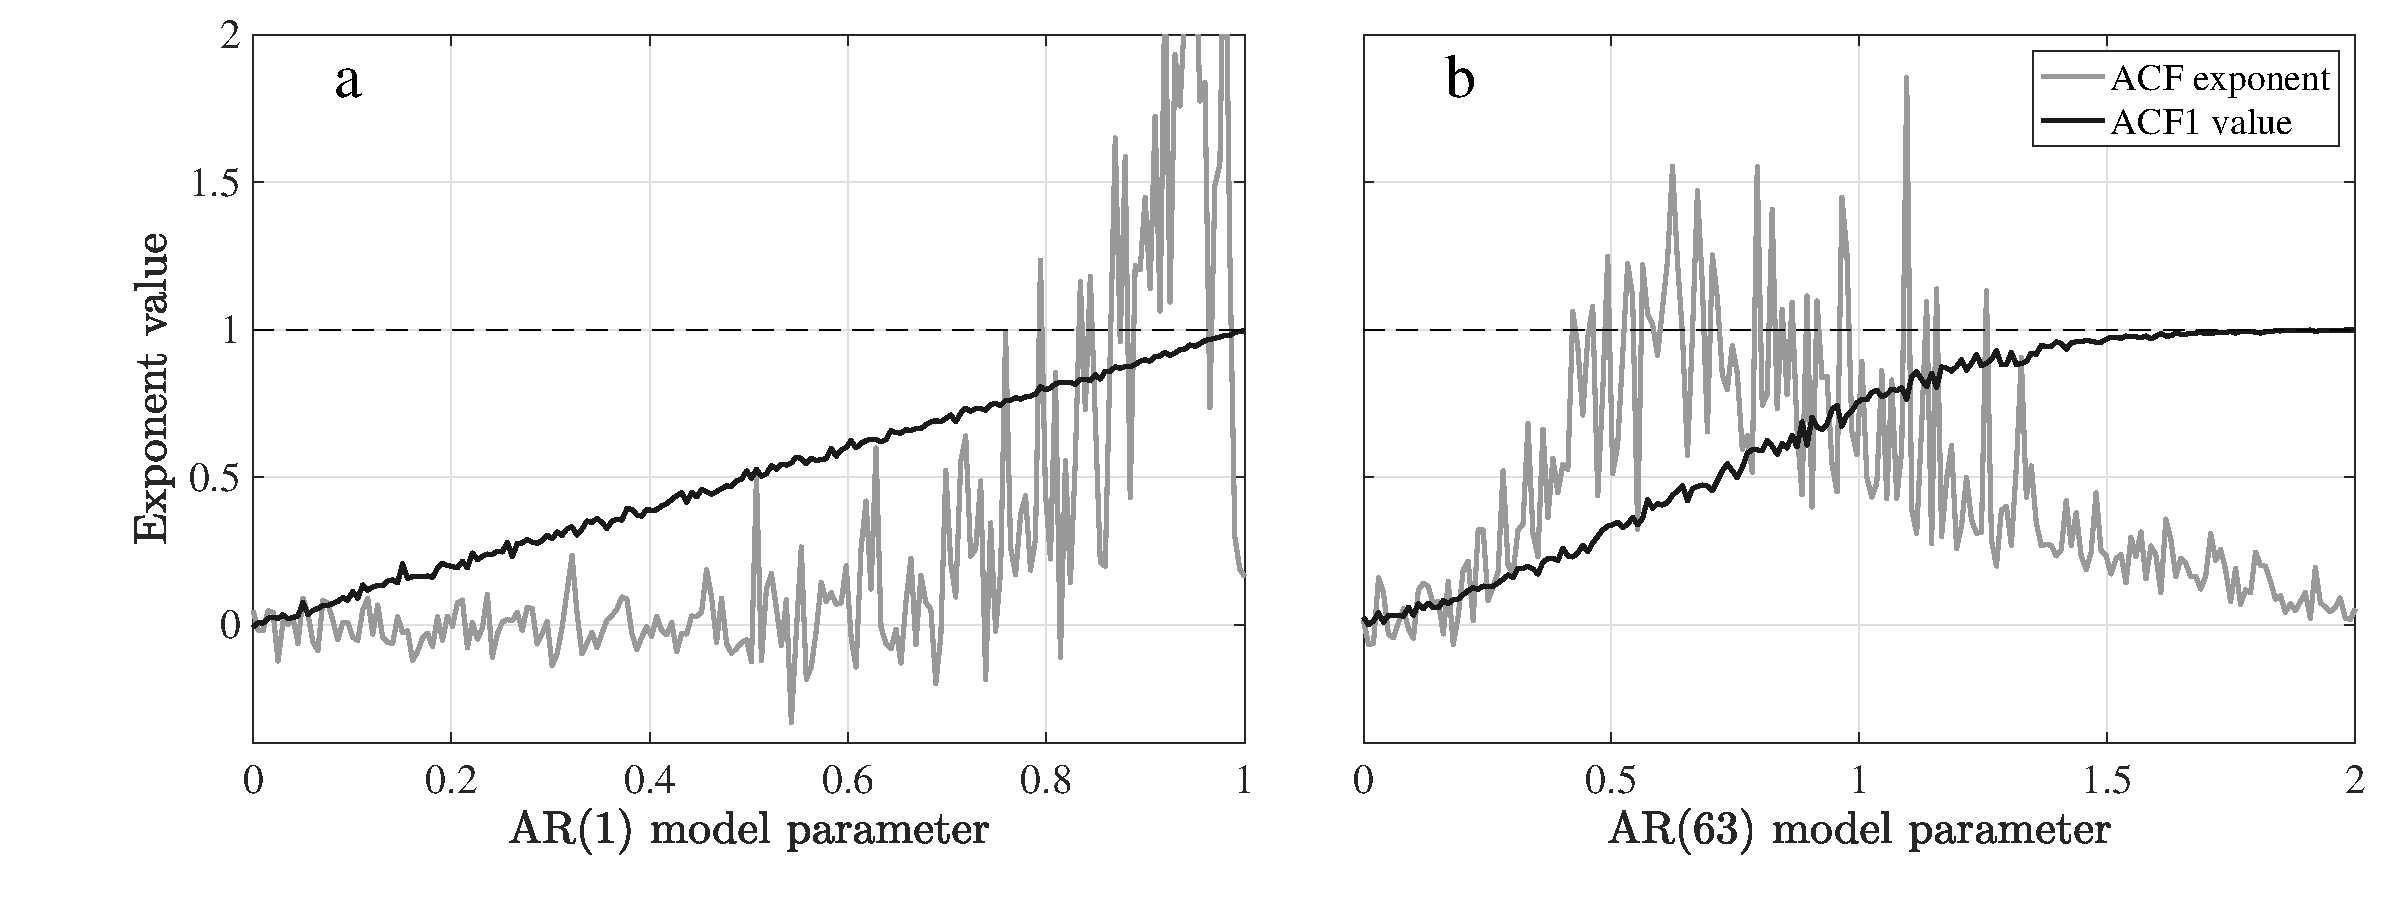
\includegraphics[width=0.9\textwidth]{f5_ACFRelationships_v2}
	\caption{ACF scaling exponent and the simple lag-1 ACF for 200 short-range correlated noise series (panel {\bf a}), and 200 long-range correlated noise series (panel {\bf b}), with varying correlation parameters.}
	\label{fig:1D:ACFrelationships}
\end{figure}






\section{Use of scaling exponents for Early Warning Signals}
%\section{Use of scaling exponents as Early Warning Signals: the ACF1, DFA and PS indicators}
\label{sec:1D:Exponents_as_EWS}


\subsection{Critical slowing down as an AR(1) process}
\label{subsec:1D:Exponents_as_EWS:CriticalSD}

The phenomenon of \emph{critical slowing down} is observed in a broad range of dynamical systems exhibiting tipping behaviour \citep{scheffer2001,lenton2008,scheffer2009,scheffer2009critical,lenton2012}. The `slowing down' to which the phrase refers is the longer and longer times taken by the system to return to the equilibrium state, given a random perturbation, in the time preceding a tipping point. At some \emph{critical} point, that is, the tipping point, the return time becomes effectively infinite\footnote{Of course, a separate tipping event may occur at which time the system returns to that original stable state.} as the system leaves that equilibrium state forever. 

The use of the autocorrelation scaling exponent as an EWS is justified by modelling a dynamical system using a one-dimensional autoregressive system:
	\begin{equation}
	\label{eqn:1D:AR1_decay_model}
		z_{n+1} = e^{-\kappa\Delta t}z_{n} + \sigma\eta_n\,,
	\end{equation}
\citep{held2004, scheffer2009} where $\sigma$ is a constant and $\eta_n$ is a white noise term. The model considers the equilibrium state $z_n=0$ as the critical mode of a system undergoing a bifurcation. The system returns to equilibrium exponentially with rate $\kappa$, the decay rate. During a bifurcation a system will undergo critical slowing down, that is, a decreasing rate $\kappa$. The autocorrelation coefficient $\alpha \equiv e^{-\kappa\Delta t}$ increases to $1$ as $\kappa$ decreases to zero. The autoregressive model parameter $\exp(-\kappa\Delta t)$, and thus the simple lag-1 autocorrelation function (ACF1), will clearly also increase as $\kappa$ decreases. The ACF1 is therefore also a possible EWS indicator and is widely used \citep{held2004,lenton2012}. As noted by \citet{scheffer2009}, it is often the case that as the autocorrelation increases so does the variance, this is true of the AR(1) process described by equation \ref{eqn:1D:AR1_decay_model} where the expectation is zero and the variance is given by
	\begin{equation}
		\text{Var}(z_n) = \frac{\sigma^2}{1-\alpha^2}\,,
	\end{equation} 
where $\alpha=\exp(-\kappa\Delta t)$ is the autocorrelation coefficient. Thus detecting an increase in variance will provide an additional EWS.

As an example of critical slowing down, we consider the bifurcating dynamical system given by the differential equation 
	\begin{equation}
		\frac{dz}{dt} = -\frac{\partial}{\partial z}U\,,
	\label{eqn:1D:ExamplePitchforkEquation}
	\end{equation}
where $U$ is the generalised potential function given by $U = z^4 + \mu z^2$, where $\mu$ is a parameter which may vary with time. If $\mu$ is positive and decreases with time, the system is an example of a pitchfork bifurcation with a decaying stable mode at $z=0$. For $\mu<0$ this mode becomes unstable and two stable modes are created at $z=\pm\sqrt{-\mu/2}$. The shape of the generalised potential function $U$ is illustrated in figure \ref{fig:intro:ChangingPotential}. Differentiating $U$, we rewrite equation \ref{eqn:1D:ExamplePitchforkEquation} as
	\begin{equation}
		\frac{dz}{dt} = -4z^3-2\mu z = f(z)\,.
	\label{eqn:1D:SimpleExamplePitchforkEquation}
	\end{equation}
We now consider the $\mu>0$ system with a small perturbation from the stable mode, that is, $z=\varepsilon$. Linearising  equation \ref{eqn:1D:SimpleExamplePitchforkEquation} using the first-order Taylor expansion around the stable mode $z=0$ gives
	\begin{equation}
		\left.\frac{dz}{dt}\right|_\varepsilon = f(\varepsilon) \approx -2\mu\varepsilon\,.
	\label{eqn:1D:TaylorExp}
	\end{equation}
So, for $\mu>0$, the system goes exponentially to zero. When $\mu=0$ the recovery rate $\m2\mu$ is zero and so the system will not recover from the small perturbation $\varepsilon$. When $\mu<0$ the mode $z=0$, as noted, is unstable and system will go exponentially away from zero. If it is assumed that a dynamical system possesses a critical mode, that is, a mode that is decaying as a result of a bifurcation, then the recovery rate of this mode will go to zero as the system takes longer (eventually infinite time, after the bifurcation) to return to the stable state after a perturbation. The tendency of the system in one direction can be measured by an increase in the lag-1 autocorrelation function (ACF1), thus this is a reasonable indicator of the decreasing decay rate. 

The hypothesis is that this critical slowing down will be seen in a wide variety of dynamical systems approaching a bifurcation. \citet{van2007} test this hypothesis with a number of ecological models and find that the intensity of the critical slowing down effect is linearly, or almost linearly, related to the distance from the tipping point in all cases.



\citet{held2004} use a rise in ACF1 as an indicator of a bifurcation in a model of North Atlantic thermohaline circulation. The measured variables are presumed to represent a dynamical system undergoing a bifurcation and therefore possessing a critical mode. In order to determine the point at which the ACF1 value rises, a method is used labelled "degenerate fingerprinting" by \citet{held2004}. The ACF1 of the data, in this case the Atlantic overturning flux, is calculated in sequential, overlapping windows so that the ACF1 value can be tracked over time. If the value is expected to rise, or begin to rise, before the tipping point, the increase in the ACF1 is an early warning signal of the tipping. 


\subsection{Early warning indicators}
\label{subsec:1D:Exponents_as_EWS:indicators}

\subsubsection{Lag-1 autocorrelation as an indicator}
{\Red
By measuring the lag-1 ACF of a time series in a sliding fixed-length time window, the value of this statistic becomes a function of time and the increase or decrease in the value over time may act as an \emph{indicator} of a tipping point. We refer to this time-dependent lag-1 ACF as the \emph{ACF1 indicator}, giving us the following definition:
}
\begin{definition} [The ACF1 indicator]
	\label{def:1D:indicator:ACF1}
	For time series data 
	\begin{equation}
		[x_t] = x_1, x_2, x_3, ..., x_N
	\end{equation}
	we create a new indicator series $[Y_t]$:
	\begin{equation}
	\label{eqn:1D:ACFfingerprinting}
		Y_t = \text{ACF}_1([x_{t-w+1},...,x_t]) ~~\text{for}~~t\geq w,
	\end{equation}
	where $w$ is the window size, typically $\leq 10\%$ of the time series length $N$. The first $w-1$ values of $[Y_t]$ are omitted. 
\end{definition}
{\Red The resulting \emph{signal}, that is, the time series of the $Y_t$ plotted over time, we refer to as an \emph{Early Warning Signal}. This method is used throughout this study and, particularly when observed physical data is used in chapter \ref{chap:cyclones}, careful attention is paid to the choice of the window size $w$. }

\subsubsection{The DFA indicator}

\citet{livina2007} modify the ACF1 indicator so that the DFA exponent is calculated instead of the lag-1 autocorrelation function in each window of data:
\begin{definition} [The DFA indicator]
	\label{def:1D:indicator:DFA}
	For time series data $[x_t] = x_1, ..., x_N$ we calculate the DFA scaling exponent $\alpha$ (see definition~\ref{def:1D:DFAexponent}) for consecutive overlapping windows $[x_{t-w+1},...,x_t]$ where $w$ is the `window size' to be determined (typically $\leq 10\%$ of the time series length $N$. We then have a sequence of values of $\alpha$:
	\begin{equation}
	\label{eqn:1D:DFAfingerprinting}
		\alpha_t = \text{DFA}([x_{t-w+1},...,x_t]) ~~\text{for}~~t\geq w\,.
	\end{equation}
	The function $\text{DFA}(\cdot)$ denotes the calculation of the order DFA exponent $\alpha$ for the truncated length-$w$ time series. The DFA indicator A(t) is this series of scaling exponent values expressed as a function of time:
	\begin{equation}
		A(t) = \alpha_t\,.
	\end{equation}
	In numerical implementations we set $A(t)=0$ for $t<w$.
\end{definition}
In this study, we consistently use the order-2 DFA exponent, but the indicator may also be used with higher orders. \citet{livina2007} test the DFA indicator method on data from a model of Atlantic overturning circulation \citep{edwards2005} and also Greenland paleotemperature records \citep{alley2000}. The DFA indicator is also compared to the ACF1 indicator \citep{lenton2012} where it is concluded that both methods offer their own pros and cons. In particular, computing the DFA exponent for every window of data is computationally expensive. 

\subsubsection{The PS exponent as an early warning indicator}
The possibility of such modification of the fingerprinting method allows us to instead use the power spectrum (PS) scaling exponent, which is obtained from the periodogram as in section \ref{subsec:1D:scaling_exponents:PS}, \citep{prettyman2018}. \citet{kleinen2003} notes already that spectral properties of the time series may also be used as tipping point indicators, in particular when the tipping point is associated with a change in the structure of the noise or a stationary system becoming non-stationary. A shift from a dominance of short-scale memory to long-scale memory, seen in the measurement of the PS scaling exponent, will be associated with a rise in autocorrelation. In this respect, therefore, the PS exponent and the ACF are related, further justifying the use of the PS exponent as an EWS. There also exists a relationship between the PS exponent and the DFA exponent \citep{heneghan2000, kantelhardt2001} as explained in section \ref{sec:1D:relationships}. We note that although \citet{heneghan2000} advises that there is no difference between the DFA and PS exponents, and that therefore it is not necessary to use both, this applies only for long-range correlated data. The relationship is investigated in section \ref{sec:1D:relationships}: while figure \ref{fig:1D:ExponentRelationships}b shows the linear relationship proposed by \citet{kantelhardt2001}, figure \ref{fig:1D:ExponentRelationships}a shows a non-linear relationship in the experiment where short-range correlated noise is used. We thus see that the relationship between the two exponents may vary depending on the nature of the data. In a system where the correlation in the time series changes over time, and trends or feedbacks affect the dynamical system, there may not exist an analytic relationship between the DFA and PS exponents and the use of one may therefore reveal information that the use of the other cannot. 

We therefore propose the use of the power spectrum indicator, alongside the DFA and ACF1 indicators. The PS exponent is estimated by calculating the negative slope of the periodogram, produced using a fast Fourier transform, in the frequency range $[10^{\m1}, 10^{\m2}]$. This is done for in a sliding window according to the fingerprinting method \citep{held2004,livina2007}. 

\begin{definition} [The PS indicator]
	\label{def:1D:indicator:PS}
	For time series data $[x_t] = x_1, ..., x_N$ we calculate the PS exponent $\beta$ (See definition \ref{def:1D:PSexponent}) for consecutive overlapping windows $[x_{t-w+1},...,x_t]$, where $w$ is the window size to be determined. We then have a sequence of $\beta$ values
	\begin{equation}
	\label{eqn:1D:PSindicator:exponent_beta}
		\beta_t = \text{PS}([x_{t-w+1},...,x_t]) ~~\text{for}~~t\geq w\,.
	\end{equation}
	The function $\text{PS}(\cdot)$ denotes, in this instance, the calculation of the power spectrum scaling exponent $\beta$ as the negative slope of the periodogram which approximates the power spectrum $S_x(f)$. The PS indicator $B(t)$ is this exponent expressed as a function of time, that is,
	\begin{equation}
		\label{eqn:1D:PSfingerprinting}
		B(t) = \beta_t\,.
	\end{equation}
	In numerical implementations we set $B(t)=0$ for $t<w$.
\end{definition}

{\Red{
		
If we consider the AR(1) model, which is used as the prototypical example of the critical slowing down phenomenon as in equation~\ref{eqn:1D:AR1_decay_model} (see section~\ref{subsec:1D:Exponents_as_EWS:CriticalSD} and \cite{scheffer2009}), we can reason that the PS exponent may provide an EWS. In that case, the critical slowing down in a system is modelled by the AR(1) process
	\begin{equation}
	\label{eqn:1D:PSindicator:AR1model}
		z_{n+1} = \mu z_{n} + \sigma\eta_n\,,
	\end{equation}
where $\eta_n$ is a white noise term and where the parameter $\mu=e^{-\kappa\Delta t}$ is determined by the \emph{decay rate} $\kappa$ which decreases to zero as the tipping point approaches, modelling the increasing time taken for a system to return to equilibrium after a small perturbation. For the PS indicator $B(t)$ to provide an EWS, we require that the value of $\beta$ changes as $\mu$ increases, that is, as the tipping point approaches. The value of $\beta$ can be obtained analytically from the power spectrum of the AR(1) process, which is given by
	\begin{equation}
	\label{eqn:1D:PSindicator:AR1powerspectrum}
		\begin{split}
		S_x(f) &= \frac{\sigma^2}{\left|1-\mu e^{\m2\pi i f}\right|^2}\\
		&= \frac{\sigma^2}{1+ \mu^2 - 2\mu\cos(2\pi f)}\,,
		\end{split}
	\end{equation}
\citep{vonstorch}. The power spectrum scaling exponent $\beta$ is then given by the negative gradient of $S_x(f)$ on a logarithmic scale, or the logarithm of $S_x(f)$ differentiated with respect to $\log f$, which gives, 
	\begin{equation}
		\beta_f = -\frac{d}{d(\log f)}\log\left[S_x(f)\right]\,.
	\end{equation}
We note that here $\beta$ depends on the frequency $f$ since the AR(1) power spectrum does not exhibit true power-law scaling; cases such as this are considered more thoroughly in section~\ref{subsec:1D:Exponents_as_EWS:nopowerlawsacaling}. In numerical calculations of the PS indicator series, the linear fit to the periodogram is taken over the interval $10^{\m2}\leq f \leq 10^{\m1}$ (see definition~\ref{def:1D:PSexponent}), the reasons for this choice of the frequency range are discussed in section~\ref{subsec:1D:Exponents_as_EWS:determining_frequency_range} and are based on taking the AR(1) process as the model of critical slowing down. 

In order to obtain a single value for $\beta$ we integrate equation~\ref{eqn:1D:PSindicator:AR1powerspectrum} over the entire range $10^{\m2}\leq f \leq 10^{\m1}$, or $\m2\leq \log f \leq\m1$, 
	\begin{equation}
	\begin{split}
		\beta &= \int_{\m2}^{\m1}-\frac{d\log\left[S_x(f)\right]}{d(\log f)}d(\log f)\\
		&= \left. \m\log\left[S_x(f)\right] \right|_{\log f = \m2}^{\m1}\\
		&= \left. \m\log\left[  \frac{\sigma^2}{1+\mu^2-2\mu \cos(2\pi f)}  \right] \right|_{\log f = \m2}^{\m1}\,,
	\end{split}
	\end{equation}
which gives 
	\begin{equation}
	\label{eqn:1D:PSindicator:PSofAR1}
		\beta = \log\left[  \frac{1+\mu^2-2\mu \cos(0.2\pi)}{1+\mu^2-2\mu \cos(0.02\pi)}  \right] \,.
	\end{equation}
This value of the PS exponent $\beta$, using this equation, is plotted in figure~\ref{fig:1D:PSofAR1}a for values of $\mu$ between $0$ and $1$. We note that $\beta$ increases from $0$ to $2$ as $\mu$ increases, that is, as the modelled critical slowing down becomes more pronounced. We therefore expect that the PS indicator $B(t)$, which tracks the value $\beta$ as a function of time, will provide an early warning signal of tipping points for which the critical slowing down phenomenon occurs, and we can expect that the PS exponent value will be $\approx 2$ when the decay rate $\kappa$ has decreased to zero ($\mu=1$ in equation~\ref{eqn:1D:PSindicator:AR1model}). In order to test the proposed relationship between the PS exponent $\beta$ and the AR(1) model parameter $\mu$, as shown in equation~\ref{eqn:1D:PSindicator:PSofAR1}, the results of an experiment are presented in figure~\ref{fig:1D:PSofAR1}b: $200$ AR(1) processes are modelled as time series of length $10^5$, each with parameter $\mu$ between $0$ and $1$. For each of the $200$ time series $X$ the PS exponent is estimated numerically in the frequency range $\m2\leq\log f\leq\m1$ and the lag-1 ACF is also calculated, the numerically-obtained PS exponent $\text{PS}(X)$ is plotted against the lag-1 autocorrelation $\text{ACF1}(X)$ in figure~\ref{fig:1D:PSofAR1}b. We note that the relationship found analytically in equation~\ref{eqn:1D:PSindicator:PSofAR1} (plotted in figure~\ref{fig:1D:PSofAR1}a) is verified by the numerical results, thus verifying the numerical method of obtaining the PS exponent (see definition~\ref{def:1D:PSexponent}).

Given a time series obtained from an AR(1) process with parameter $\mu$, that is,
\begin{equation}
	z_{n+1} = \mu z_n + \eta_n,
\end{equation}
with $\eta_n$ independent Gaussian white noise terms, we can reconstruct the value $\mu$ from the time series only by calculating the PS exponent $\beta$ in the frequency range $\m2\leq\log f\leq\m1$. We simply solve equation~\ref{eqn:1D:PSindicator:PSofAR1} for $\mu$ to obtain
\begin{equation}
	\label{eqn:1D:PSindicator:reconstruct_mu}
	\mu\approx b-\sqrt{b^2-1}~~~\text{where}~~~ b = \frac{\cos(0.2\pi)-10^\beta \cos(0.02\pi)}{1-10^\beta}.
\end{equation}
This result may appear counter-intuitive given that the power spectrum of the AR(1) process does not actually exhibit power-law scaling, but we see clearly in figure~\ref{fig:1D:PSofAR1} that the values obtained using this equation correlate with the lag-1 autocorrelation. This relationship, and the relevance of the PS indicator in systems where the power spectrum does not have power-law scaling, are investigated further in sections~\ref{subsec:1D:Exponents_as_EWS:nopowerlawsacaling} and~\ref{subsec:1D:Exponents_as_EWS:determining_frequency_range}.
}}

\begin{figure}
	% plotted using the Matlab script 'PSofAR1.m'
	\centering
	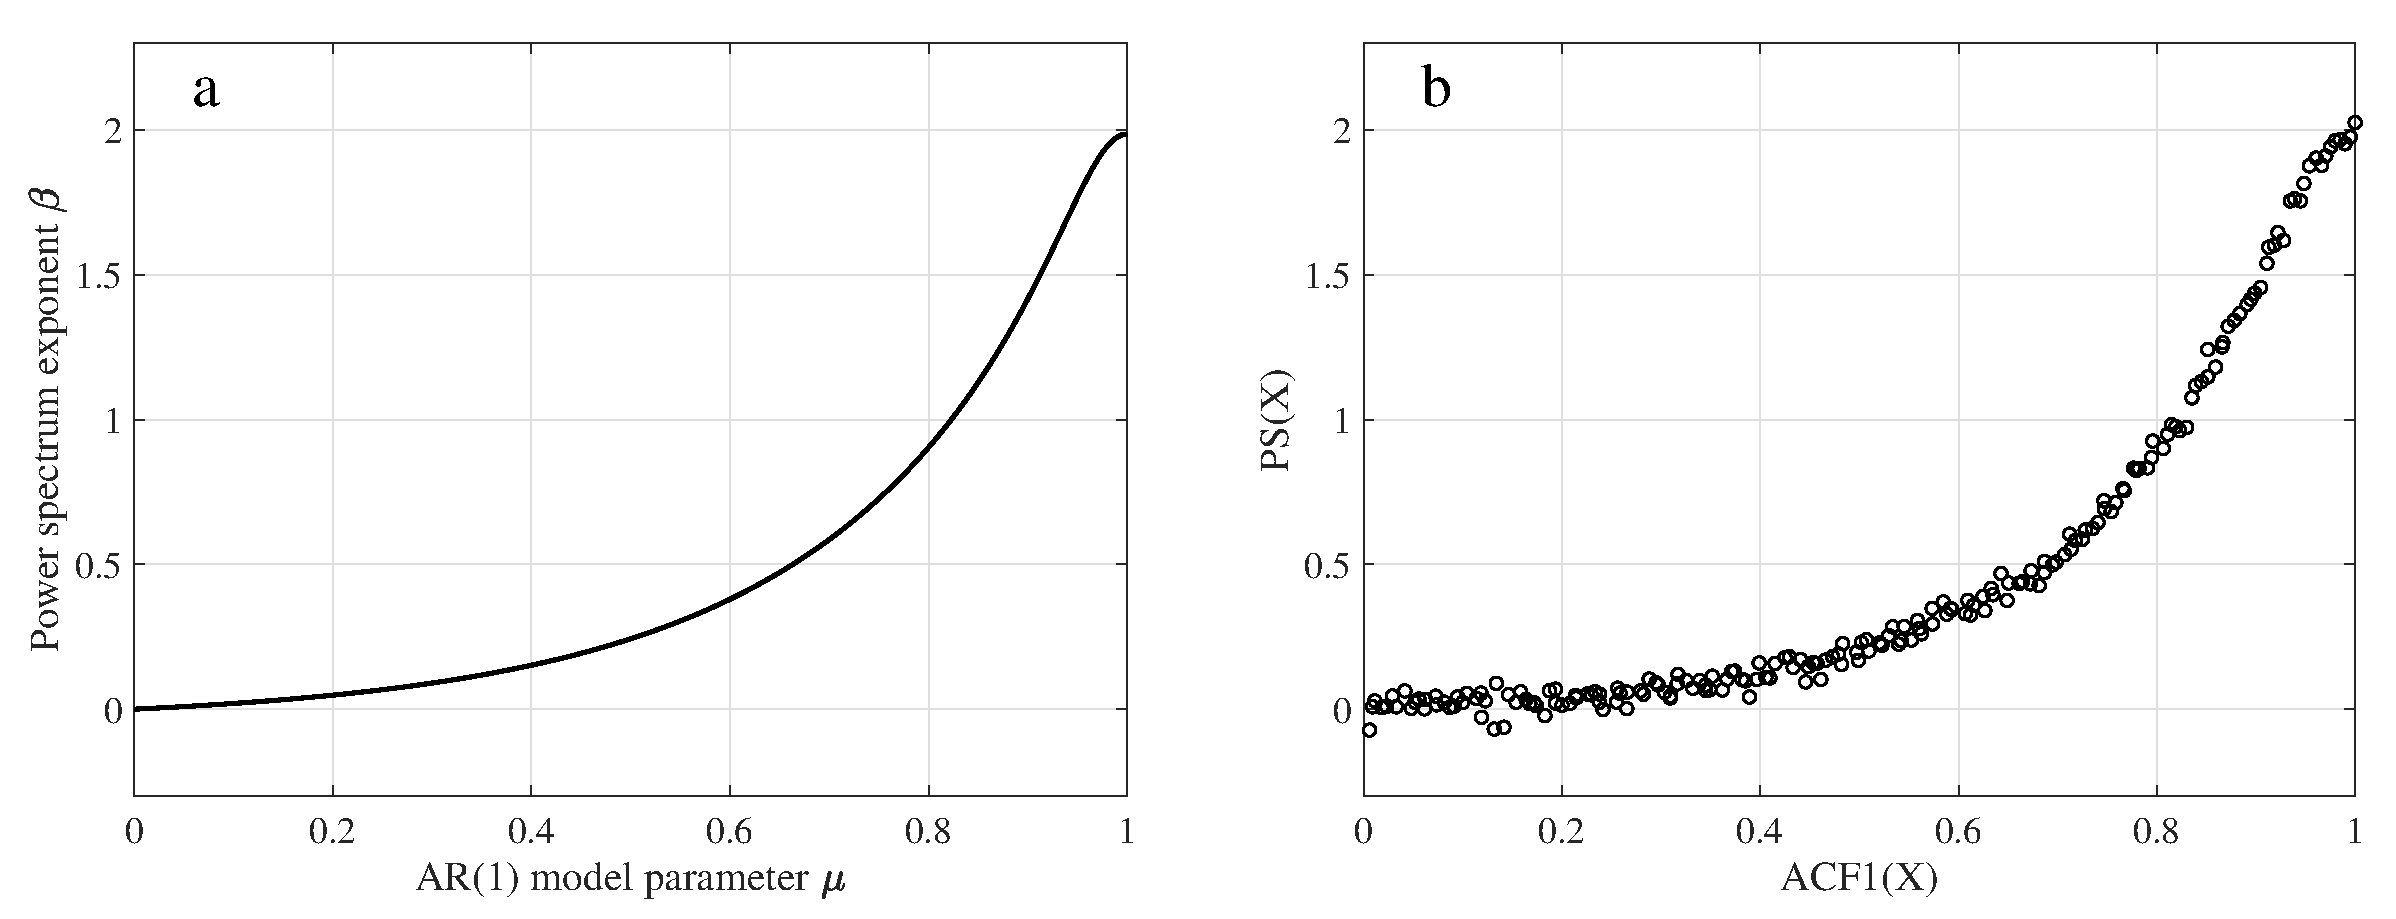
\includegraphics[width=0.9\linewidth]{PSofAR1}
	\caption{\label{fig:1D:PSofAR1}
		{\Red Panel {\bf a}: The relationship between the PS scaling exponent $\beta$ and the parameter $\mu$ of the AR(1) process is plotted for $0\leq\mu\leq 1$ (see equation~\ref{eqn:1D:PSindicator:PSofAR1}). Panel {\bf b}: The PS exponent and lag-1 autocorrelation is calculated for $200$ AR(1) time series $X$ of length $10^5$ and the results plotted against each other. The relationship between these numerically-obtained values confirms the derivation of equation~\ref{eqn:1D:PSindicator:PSofAR1} and the accuracy of the numerical methods.}
	}
\end{figure}

\subsubsection{The ACF scaling exponent as an early warning indicator}

{\Red{

As we have defined the DFA indicator $A(t)$ based on the DFA scaling exponent $\alpha$, and the PS indicator $B(t)$ based on the PS scaling exponent $\beta$, we have neglected the ACF scaling exponent $\gamma$ (see definition~\ref{def:1D:ACFexponent}), from which we might define the ACF scaling indicator $\Gamma(t)$ in much the same way. However, this is not often used as an early warning indicator in the literature and the DFA scaling exponent has been developed as a superior alternative to the ACF scaling exponent \citep{kantelhardt2001}: this has since been used successfully as an early warning indicator \citep{livina2007}. When testing the effectiveness of the novel PS indicator we therefore use the DFA indicator as a benchmark.

Another useful benchmark test for a novel indicator is whether it is effective in detecting a change in the model parameter of the AR(1) process, since this is used as a model of critical slowing down (see section~\ref{subsec:1D:Exponents_as_EWS:CriticalSD}). In figure~\ref{fig:1D:ACFrelationships} we have already demonstrated the superior performance of the simple lag-1 autocorrelation over the ACF scaling exponent, and the ACF1 indicator is used throughout this thesis for comparison with the PS indicator. For these reasons, we do not use what we might call the `ACF scaling indicator' but look to the ACF1 indicator and the DFA indicator instead.

}}

\subsection{Early warning indicators in the absence of power-law scaling}
\label{subsec:1D:Exponents_as_EWS:nopowerlawsacaling}

{\Red{
The definitions of all scaling exponents, and thus early warning indicators, assume the existence of power-law scaling. For example, in the case of the PS exponent we assume the power spectrum $S(f)$, which is approximated by the periodogram, is of the form $S(f)\sim f^{-\beta}$ for some exponent $\beta$, and it is this value that we seek to measure. However, it is unlikely that we will find true power-law scaling like this in dynamical systems or data from real-life processes unless we are dealing with pure white noise or a pure random walk. Indeed we note that the common stochastic model, the AR(1) process, with which we model critical slowing down \citep{scheffer2009critical}, does not even have true power-law scaling in the power spectrum. 

In this section we show that it is still a valuable exercise to measure the PS exponent in cases in which there is no true power-law scaling. In particular, we focus on cases for which there is \emph{crossover} in the power spectrum, that is, when the power spectrum follows one power-law scaling relationship at low frequencies and another at higher frequencies, with a crossover at some midpoint. In the following  section~\ref{subsec:1D:Exponents_as_EWS:determining_frequency_range} we concentrate specifically on the AR(1) model which is of importance to tipping point research, and which also contains a power spectrum crossover.
}}

\subsubsection{Power spectra containing crossovers}
{\Red{
To create a time series with a clear crossover in the power spectrum we take the sum of a Gaussian white noise series $\eta_t$ and red noise (random walk) series $W_t$ defined by the relation $W_t = W_{t-1} + \zeta_t$, where $\zeta_t$ are a Gaussian white noise series independent of $\eta_t$. Thus the terms of the series are given by
	\begin{equation}
	\label{eqn:1D:crossoverfunction}
		z(t) = \left(\sum_{\tau=0}^t \zeta_\tau\right) + \mu\eta_t\,,
	\end{equation}
where $\mu$ is a parameter modifying the variance of the white noise terms $\eta_t$. Due to the linearity of the Fourier transform we are able to calculate the power spectrum $S_z(f)$ of this series given that we know already
	\begin{equation}
	\label{eqn:1D:powerspectrum_white}
		S_{\mu\eta}(f) = \left| \mu\hat{\eta}(f) \right|^2 = \mu^2
	\end{equation}
since $\hat{\eta}(f)=1$, and
	\begin{equation}
	\label{eqn:1D:powerspectrum_red}
		S_{W}(f) = \left| \hat{W}(f) \right|^2 = \left|\frac{1}{2\pi f}\right|^2 = \frac{1}{4\pi^2}f^{\m2}.
	\end{equation}
Combining the two series we have
	\begin{equation}
	\begin{split}
		S_z(f) &= \left| \hat{z}(f) \right|^2\\
		&= \left| \hat{W}(f) + \mu\hat{\eta}(f) \right|^2\\
		&= \left| \frac{1}{2\pi f} + \mu\right|^2\\
		\label{eqn:1D:powerspectrum_cross}
		&= \frac{1}{4\pi^2}f^{\m2} + \frac{\mu}{2\pi}f^{\m1} + \mu^2\,.
	\end{split}
	\end{equation}
}}

\begin{figure}
	\centering
	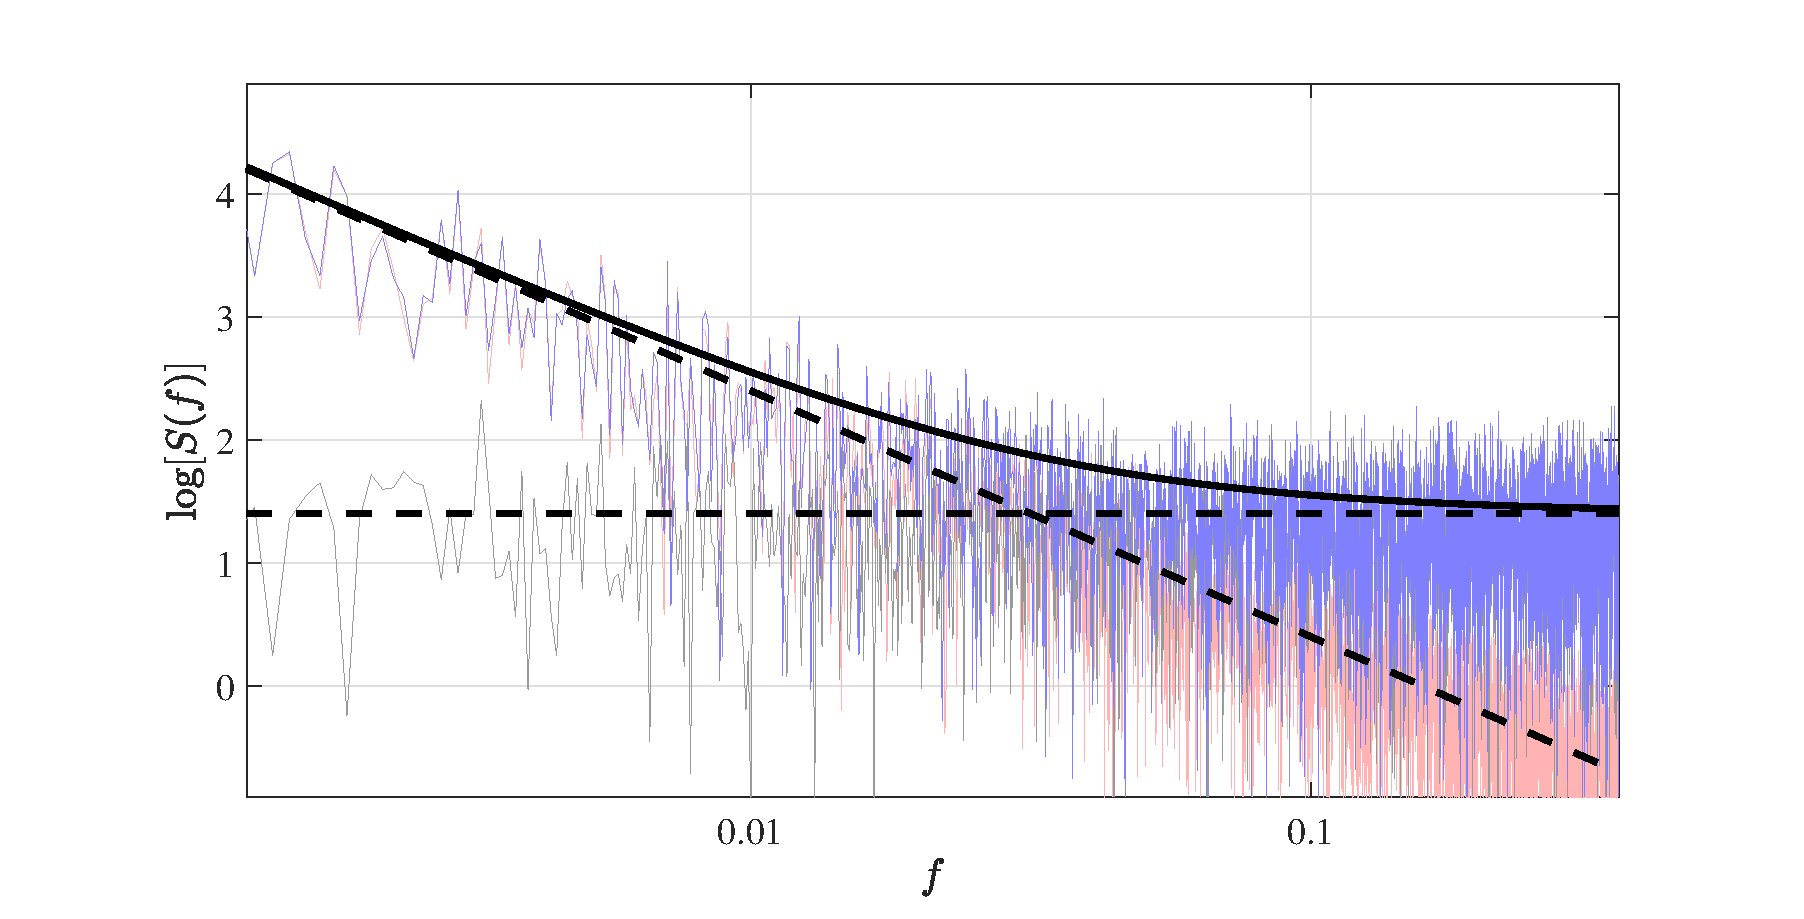
\includegraphics[width=\linewidth]{crossover1}
	\caption{\label{fig:1D:crossover1}
		{\Red Scaling crossover in the power spectrum of the sum of red and white noise series. Showing the power spectrum of the series $z(t)$ (solid black line, see equation~\ref{eqn:1D:crossoverfunction}) imposed over the periodogram (blue). Also showing the power spectrum of white and red noise (dashed black lines) and their periodograms (grey and red respectively). The crossover occurs at $f=10^{-3/2}$ (see equation~\ref{eqn:1D:crossoverfrequency}).}
	}
\end{figure}

{\Red{
In figure~\ref{fig:1D:crossover1} the power spectra of white noise $\mu\eta_t$ and red noise $W_t$, given by equations~\ref{eqn:1D:powerspectrum_white} and~\ref{eqn:1D:powerspectrum_red} respectively, are shown (dashed lines) imposed over the periodograms of computed instances of these series (shown in grey and red respectively). In this case the value 
	\begin{equation}
		\mu = \frac{10^{3/2}}{2\pi}
	\end{equation}
has been chosen so that the intersection of the two curves, given by equations~\ref{eqn:1D:powerspectrum_white} and~\ref{eqn:1D:powerspectrum_red} is given by 
	\begin{align}
	\label{eqn:1D:crossoverfrequency}
		\begin{split}
		\frac{1}{4\pi^2}f^{\m2} &= \mu^2,\\
		\frac{1}{2\pi}f^{\m1} &= \mu,\\
		\frac{1}{2\pi}f^{\m1} &= \frac{10^{3/2}}{2\pi},\\
		f &= 10^{\m3/2}\,,
		\end{split}
	\end{align}
which is the midpoint of the values $f=0.01$ and $f=0.1$ on the logarithmic scale. In figure~\ref{fig:1D:crossover1} we also see the power spectrum of the function $z(t)$, given by equation~\ref{eqn:1D:powerspectrum_cross} (solid line), and the periodogram of an instance of the time series (shown in blue). This time series is simply the sum of the white noise and red noise series. We note that the periodogram of $z$ entirely overlaps the periodogram of the red noise series $W$ for small values of $f$, and overlaps the periodogram of the white noise series $\eta$ for large values of $f$. 
}}

\subsubsection{Applying the PS indicator}
	\begin{figure}
		\centering
		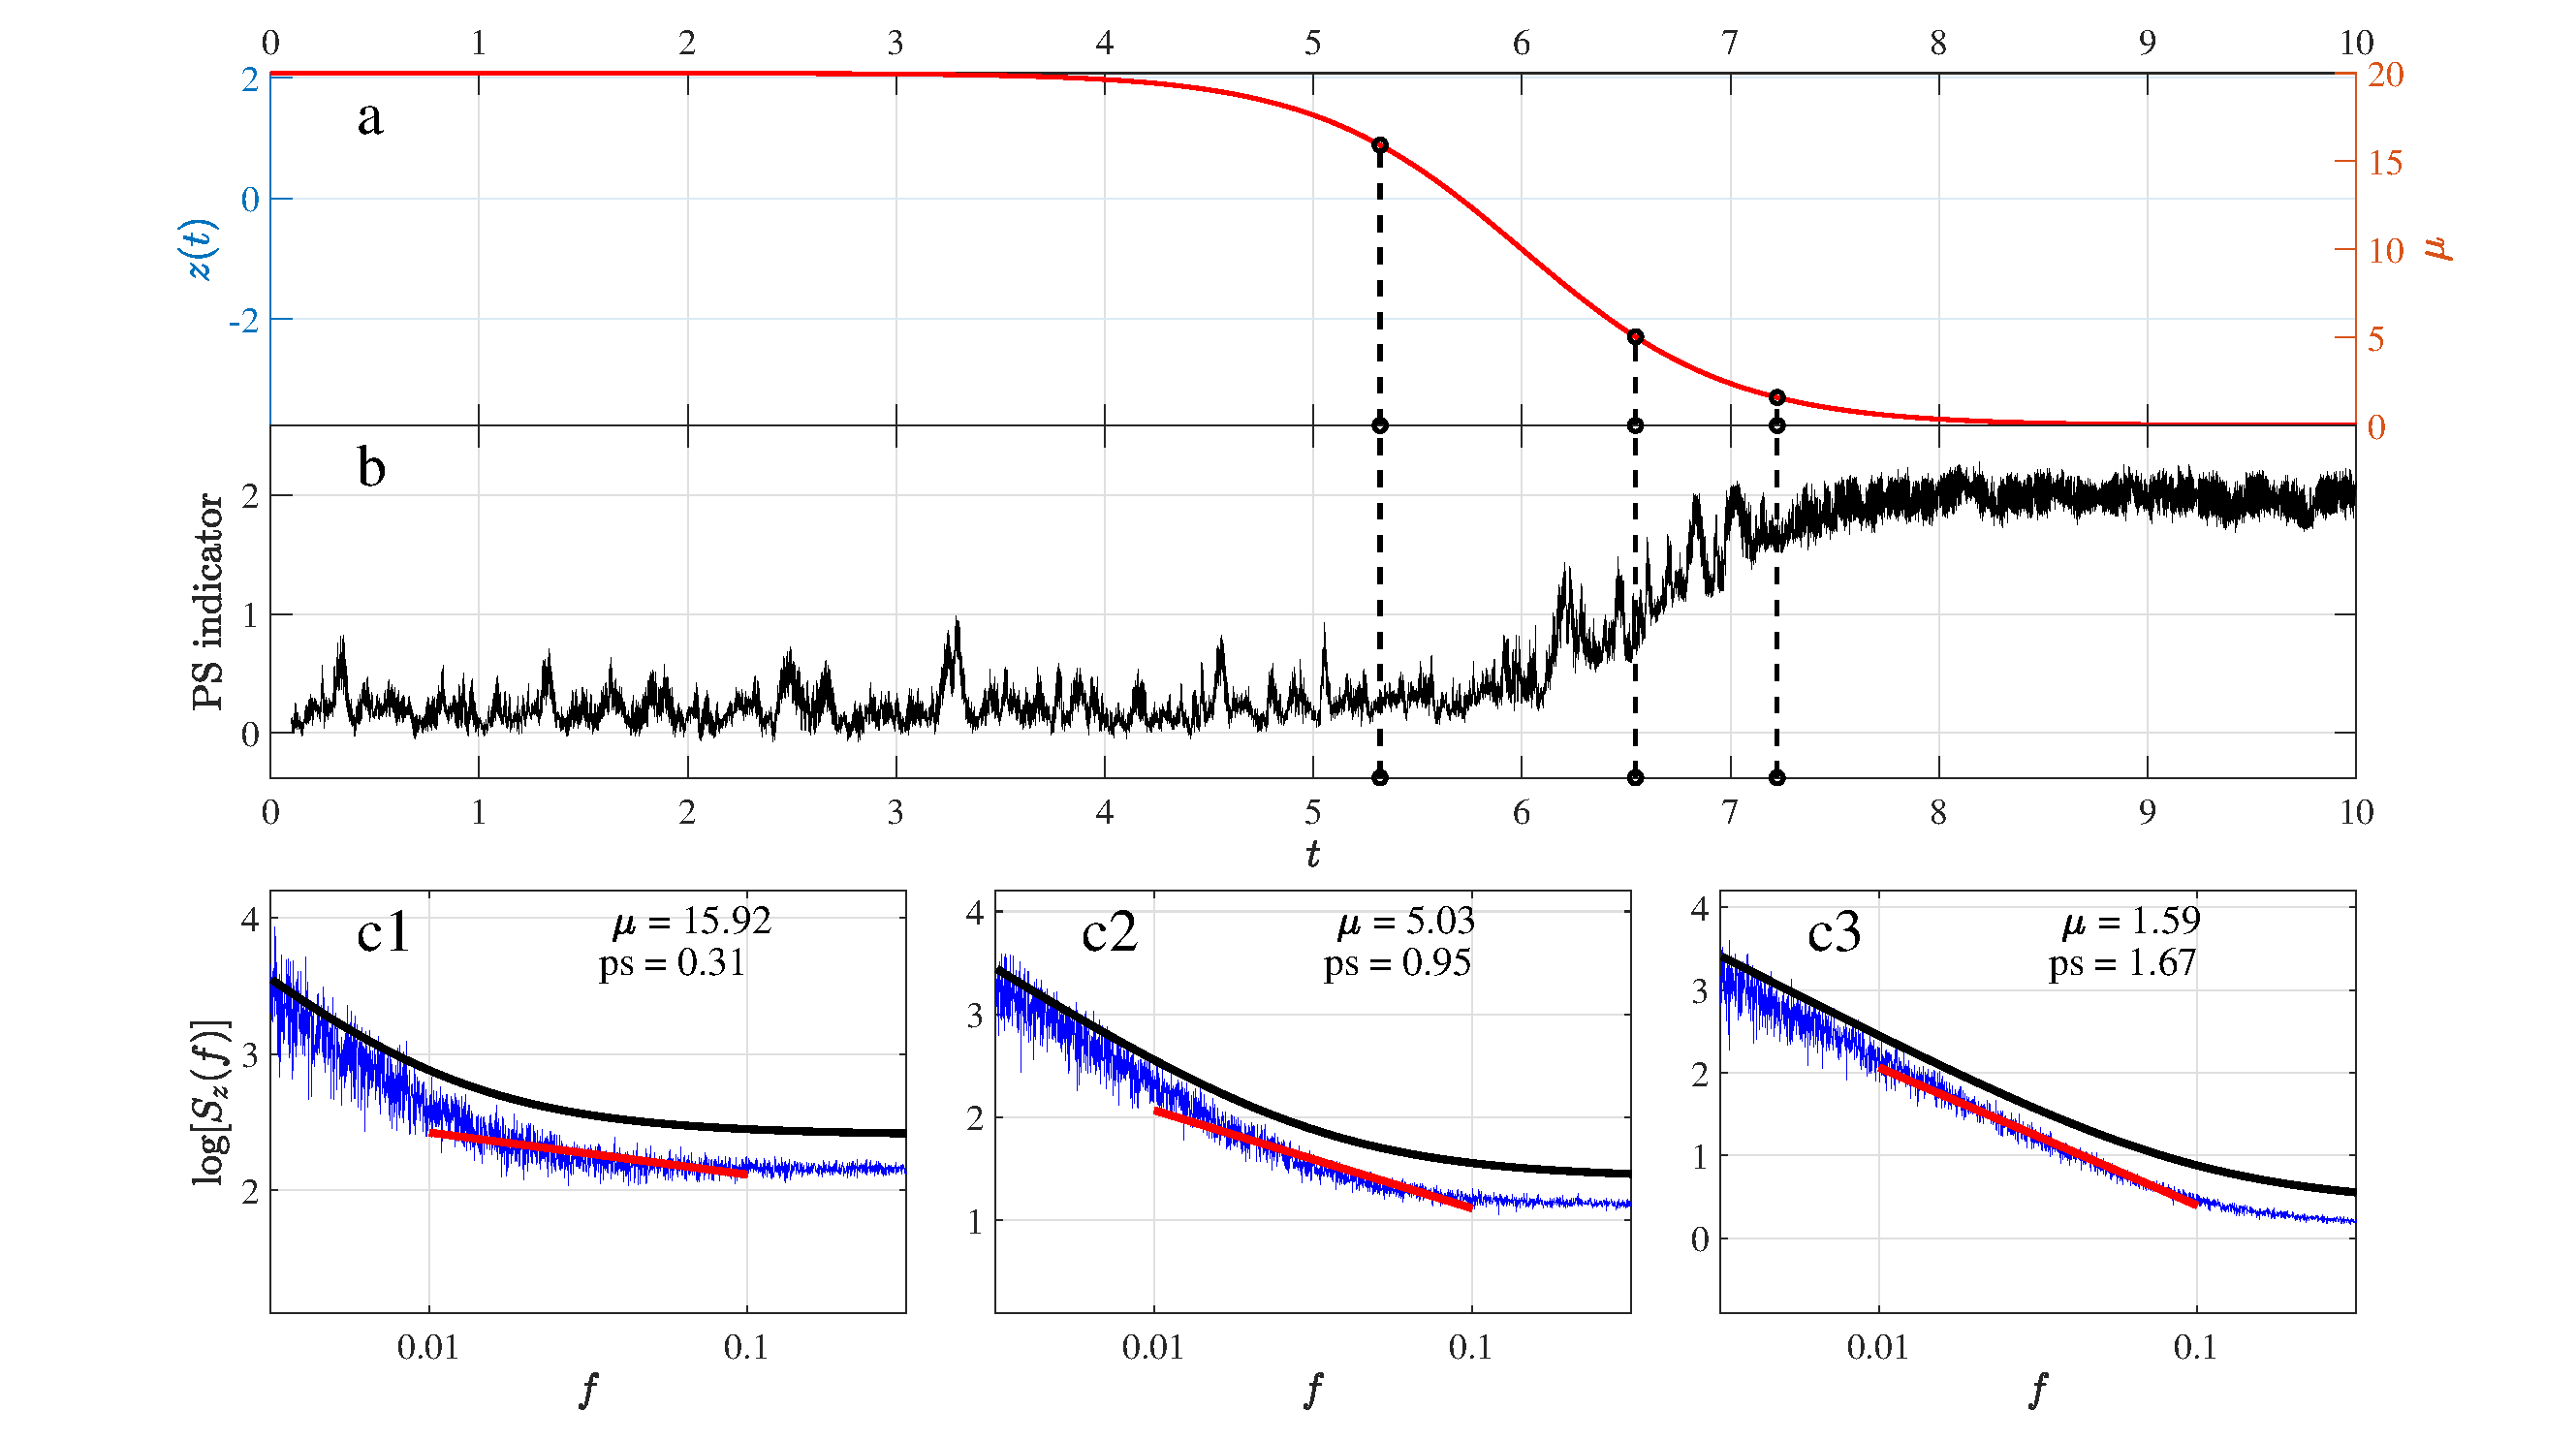
\includegraphics[width=\linewidth]{crossover2_decrease}
		\caption{\label{fig:1D:crossover2}
			{\Red Power spectrum indicator of the sum of white noise and red noise series with decreasing white noise component. Panel {\bf a}: The time series $z(t)$ (blue, left $y$-axis) and the standard deviation $\mu$ of the white noise component (red, right $y$-axis). The dashed black lines show times at which the crossover point is at the lower end, the centre, and the upper end of the frequency range in which the PS indicator is measured. Panel {\bf b}: The PS indicator in a sliding window $1\%$ of the length of the time series. Panels {\bf c}: Depictions of the periodograms of $z(t)$ when the crossover point is at the lower end, the centre, and the upped end of the measured frequency range (panels c1, c2, c3 respectively). The power spectrum (black) and the linear fit to the periodogram (red) and also shown.}
		}
	\end{figure}
{\Red{
The power spectrum of $z(t)$, given by equation~\ref{eqn:1D:powerspectrum_cross}, does not exhibit simple power-law scaling, since there is no value $\xi$ for which 
	\begin{equation}
		S_z(cf) = c^\xi S_z(f)\,,
	\end{equation}
and so the power spectrum is not simply a straight line in the log-log plot (figure~\ref{fig:1D:crossover1}). However, this does not mean that there is no value in applying the Power Spectrum indicator, which simply fits a straight line to the periodogram to obtain a single value $\xi$. When applying the PS indicator to dynamical systems with tipping behaviour it is not the exact value of the indicator that is of interest but the change in the value over time as the indicator is applied in a sliding window on the time series. In particular we are concerned with the detection of critical slowing down in the time before a tipping point is reached which is characterised by an increase in the autocorrelation scaling exponent, or a ``reddening'' of the power spectrum as the return time around a stable state increases. 

In figure~\ref{fig:1D:crossover2}a we have plotted the series $z(t)$ given by equation~\ref{eqn:1D:crossoverfunction}, the sum of a red noise and a white noise series with scaling crossover (blue line, left $y$-axis). In this case the value of the parameter $\mu$ changes with time and is described by the function
	\begin{equation}
		\mu(t) = 10-10\tanh(t-6),
	\end{equation}
so that $\mu\rightarrow20$ as $t\rightarrow-\infty$ and $\mu\rightarrow0$ as $t\rightarrow\infty$. This function is plotted alongside the time series in figure~\ref{fig:1D:crossover2}a (red line, right $y$-axis). We note that the value of $f$ at which the crossover occurs in the power spectrum is given by 
	\begin{equation}
		f_\text{c} = \frac{1}{2\pi\mu},
	\end{equation}
(see equation~\ref{eqn:1D:crossoverfrequency}) and therefore varies with the value of $\mu$. For this experiment, when applying the PS indicator, we have chosen to estimate the slope of the periodogram in the frequency range $10^{\m2}\leq f \leq 10^{\m1}$. For large values of $\mu$, i.e. $\mu>100/2\pi\approx15.9$ we have $f_\text{c}<0.01$ and so the crossover point lies outside of the measurement range, in which case the PS indicator will have a value similar to that of white noise (zero) since the red noise aspect of the periodogram is not measured. Similarly, for $\mu<10/2\pi\approx1.59$ we have $f_\text{c}>0.1$ and in this case only the red noise aspect of the periodogram is measured. The times at which these two values of $\mu$ occur, which are the times that the crossover point enters and then leaves the measured frequency range, are marked by vertical dashed lines on figure~\ref{fig:1D:crossover2}a. The centre dashed line marks the point in time at which $\mu = 10^{3/2}/2\pi\approx5.03$, when the crossover point appears directly in the centre of the measured frequency range in the logarithmic scale (see equation~\ref{eqn:1D:crossoverfrequency}). 

In figure~\ref{fig:1D:crossover2}b the PS indicator is plotted in a sliding window of length $10^4$ points, which is $1\%$ of the length of the time series, $N=10^6$. The three dashed vertical lines are continued from figure~\ref{fig:1D:crossover2}a and show the times at which the crossover point enters, is in the centre of, and leaves the frequency range in which the PS indicator is measured. We note that the PS indicator rises correspondingly as the value of $\mu$ decreases, that is, as the variance of the white noise component of the system decreases, leaving only the red noise component as $\mu\rightarrow0$, the ``redness'' of the data increases. Thus, we are able to detect an increasing reddening of time series using the PS indicator, even when there is no simple power-law scaling due to the presence of a crossover. 

In figure~\ref{fig:1D:crossover2}c1, c2 and c3 three periodograms are shown, these are periodograms of a time series $z(t)$ of length $10^5$ with a constant value of $\mu$. The three values of $\mu$ used are the values marked in figure~\ref{fig:1D:crossover2}a with dashed lines, at which points the crossover is at the lower end (panel c1), the centre (panel c2), and the upper end (panel c3) of the measured frequency range. Also shown over the three periodograms are the PS indicator estimation (red line) and the analytically calculated power spectrum (black curve) in equation~\ref{eqn:1D:powerspectrum_cross}. This power spectrum in each case is a smooth curve, not the union of two lines depicted in figure~\ref{fig:1D:crossover1}, and the PS indicator is still influenced by the decreasing ``red'' part of the power spectrum a short time before the crossover point enters the range $10^{\m2}\leq f \leq 10^{\m1}$, and similarly the periodogram is still influenced by the flat ``white'' part of the spectrum for a short time after the crossover point leaves this range. In figure~\ref{fig:1D:crossover2}c1 we see the influence of the red noise when the crossover point is precisely at the lower bound of the range, although the white noise is still dominant. The PS indicator for this value of $\mu$ is $0.36$; this value is closer to zero for even larger values of $\mu$ where the red noise has a much smaller variance than the white noise and has far less influence on the shape of the periodogram.
}}


\subsection{Determining the frequency range of the PS exponent}
\label{subsec:1D:Exponents_as_EWS:determining_frequency_range}
{\Red
The definition of the PS exponent (definition~\ref{def:1D:PSexponent}) relies upon measuring the gradient of the periodogram as a function of frequency plotted on logarithmic axes. The estimation of the gradient may be done in over the whole domain $0\leq f\leq 1/2$, or over some subset. In cases where true power-law scaling does not exist, the choice of the range of frequencies over which the gradient is measured may significantly affect the result though, as demonstrated in section~\ref{subsec:1D:Exponents_as_EWS:nopowerlawsacaling}, performing the analysis in such cases may still be worthwhile. It is necessary, therefore, to choose a range of frequencies most likely to give a visible indicator in the presence of a tipping point. 

Up to this point we have referred to the use of the range $10^{\m2}\leq f\leq 10^{\m1}$ as most suitable, citing the choice of the time scale $10^1 \leq t\leq 10^2$ used when calculating the ACF and DFA exponents \citep{livina2007} as a model. In this section we calculate the PS exponent of an AR(1) process, which is of importance in a tipping point context since it models the critical slowing down phenomenon \citep{scheffer2009}, and by doing so show that the optimal range in which to measure the PS exponent is $10^{\m2}\leq f\leq 10^{\m1}$, provided that detecting a `reddening' of the noise in the AR(1) process is the aim. 

The stochastic process used as an example in the previous section, the sum of a red noise process and a white noise process, was chosen for its clearly visible power spectrum crossover. We now look at the discrete AR(1) process $x_t$ defined by the equation
	\begin{equation}
		x_t = \mu x_{t-1} + \eta_t\,,
	\end{equation}
where $\eta_t$ is a Gaussian white noise process with variance $\sigma^2$ and $\mu$ is a parameter which, in this experiment, is in the range $0\leq \mu \leq 1$. For $\mu=0$ this is a pure Gaussian white noise process while for $\mu=1$ this is a random walk (red noise). As $\mu$ increases from $0$ to $1$ as a function of time we expect to see this noise process become `redder': developing long-term memory, which is not present in a white noise signal, and therefore developing properties similar to those of the random walk. Of course the lag-1 autocorrelation function will increase with $\mu$, but in this example we inspect the power spectrum, which is given by
	\begin{equation}
	\label{eqn:1D:AR1process_powerspectrum}
		S_x(f) = \frac{\sigma^2}{1+ \mu^2 - 2\mu\cos(2\pi f)}\,,
	\end{equation}
\citep{vonstorch}, a reprinting of equation~\ref{eqn:1D:PSindicator:AR1powerspectrum} (page~\pageref{eqn:1D:PSindicator:AR1powerspectrum}). The derivation of this equation assumes that $\mu$ is constant over time whereas we are interested in cases where $\mu$ is increasing (or otherwise changing). However, we are only interested in the shape of the power spectrum in time windows which are short relative to the whole time series, so that we can track the changing shape, and we assume $\mu$ is constant within each window. That is, we assume $\mu$ changes slowly relative to the dynamics of the AR(1) process. 
 
For the purposes of tipping point analysis we are interested in the \emph{Power Spectrum Scaling Exponent} which we define as the value $\beta$ such that the power spectrum satisfies the scaling relationship
	\begin{equation}
		S_x(f) \sim f^{\m\beta}.
	\end{equation}
For power spectra where $\beta$ exists, that is, where there is a global power-law scaling relationship, the value can be obtained by taking the negative value of the gradient of the log-log plot. Given a time series, we can estimate the value $\beta$ by measuring the negative gradient of the log-log plot of the periodogram. For time series of processes whose power spectra do not satisfy a power-law scaling relationship, and therefore no single number $\beta$ exists, we are still able to measure the gradient of the power spectrum at a particular value of $f$ (or averaged over a range of values). We refer to this specific exponent $\beta_f$ as the \emph{Power Spectrum Exponent}, although it is not a scaling exponent in the sense that the power spectrum actually satisfies a power-law scaling relationship. 

In the case of the AR(1) process we calculate the specific PS exponent $\beta_f$ as the negative gradient of the log-log plot of the power spectrum (where $\log$ refers to the base-$10$ logarithm $\log_{10}$), which we obtain by differentiating $\log[S_x(f)]$ with respect to $\log f$:
	\begin{align}
		\begin{split}
		\beta_f := \text{PS exponent} &= -\frac{d}{d(\log f)}\log[S_x(f)]\\
		&= -\frac{d}{d(\log f)}\log\left[\frac{\sigma^2}{1+ \mu^2 - 2\mu\cos(2\pi f)}\right]\\
		&= -\frac{d}{du} \log\left[\frac{\sigma^2}{1+\mu^2-2\mu\cos(2\pi 10^u)}\right]\\
		&= \frac{d}{du} \log\left[1+\mu^2-2\mu\cos(2\pi 10^u)\right]\\
		&= \frac{1}{\ln(10)}\cdot\frac{4\pi \mu \ln(10) 10^u \sin(2\pi 10^u)}{1+\mu^2-2\mu\cos(2\pi 10^u)}\\
		&= \frac{4\pi \mu f \sin(2\pi f)}{1+\mu^2-2\mu\cos(2\pi f)}\,,
		\end{split}
	\end{align}
where we have used the substitution $u = \log_{10}f$ to simplify the calculation. This gradient may then be evaluated at a particular value of $f$ (or, rather, in the case of the periodogram, estimated by a linear fit in a particular range of $f$ values). What we refer to as the \emph{Power Spectrum Indicator} is the value of this PS exponent as a function of time,
	\begin{equation}
	\label{eqn:1D:AR1_psindicator}
		B_f(t):=~\text{PS indicator} = \frac{4\pi \mu f \sin(2\pi f)}{1+\mu^2-2\mu\cos(2\pi f)},
	\end{equation}
where the $t$ dependence comes from the fact that $\mu = \mu(t)$ is a function of time. We are now able to take the $t$ derivative:
	\begin{equation}
		\frac{d}{dt}B_f(t) = \frac{4\pi f \sin(2\pi f)\dot\mu(1-\mu^2)}{1+\mu^2-2\mu\cos(2\pi f)}.
	\end{equation}
Equating this to zero, assuming $\mu(t)$ is not a constant function ($\dot\mu \neq 0$), we find the maximum value of the PS indicator occurs when $\mu=1$ (when the AR(1) process is a random walk) at which point the PS indicator $B_f$ has a maximal value of 2 which occurs as $f$ approaches zero, that is,
	\begin{equation}
	\label{eqn:1D:maximumPSindicator_AR1}
		\max[B_f] = \frac{2\pi f \sin(2\pi f)}{1-\cos(2\pi f)} ~~\xrightarrow[f\rightarrow 0]{}~ 2\,.
	\end{equation}
For larger values of $f$ the maximum indicator value is not close to the maximal value of 2. For $f = 0.1$ we have $\max[B_{0.1}] = 1.93$, whereas for $f = 0.38$ already the value is significantly less:  $\max[B_{0.38}] = 1$. In cases where the PS indicator is being estimated using a noisy periodogram it is essential that the increase in the indicator value as critical slowing down occurs (that is, as $\mu$ increases from 0 to 1) is easily observable. For this reason, when we estimate the PS scaling exponent, a frequency $\log(f)\leq \m1$ should be used in order to be able to observe the largest increase in the PS indicator.
}

\begin{figure}
	\centering
	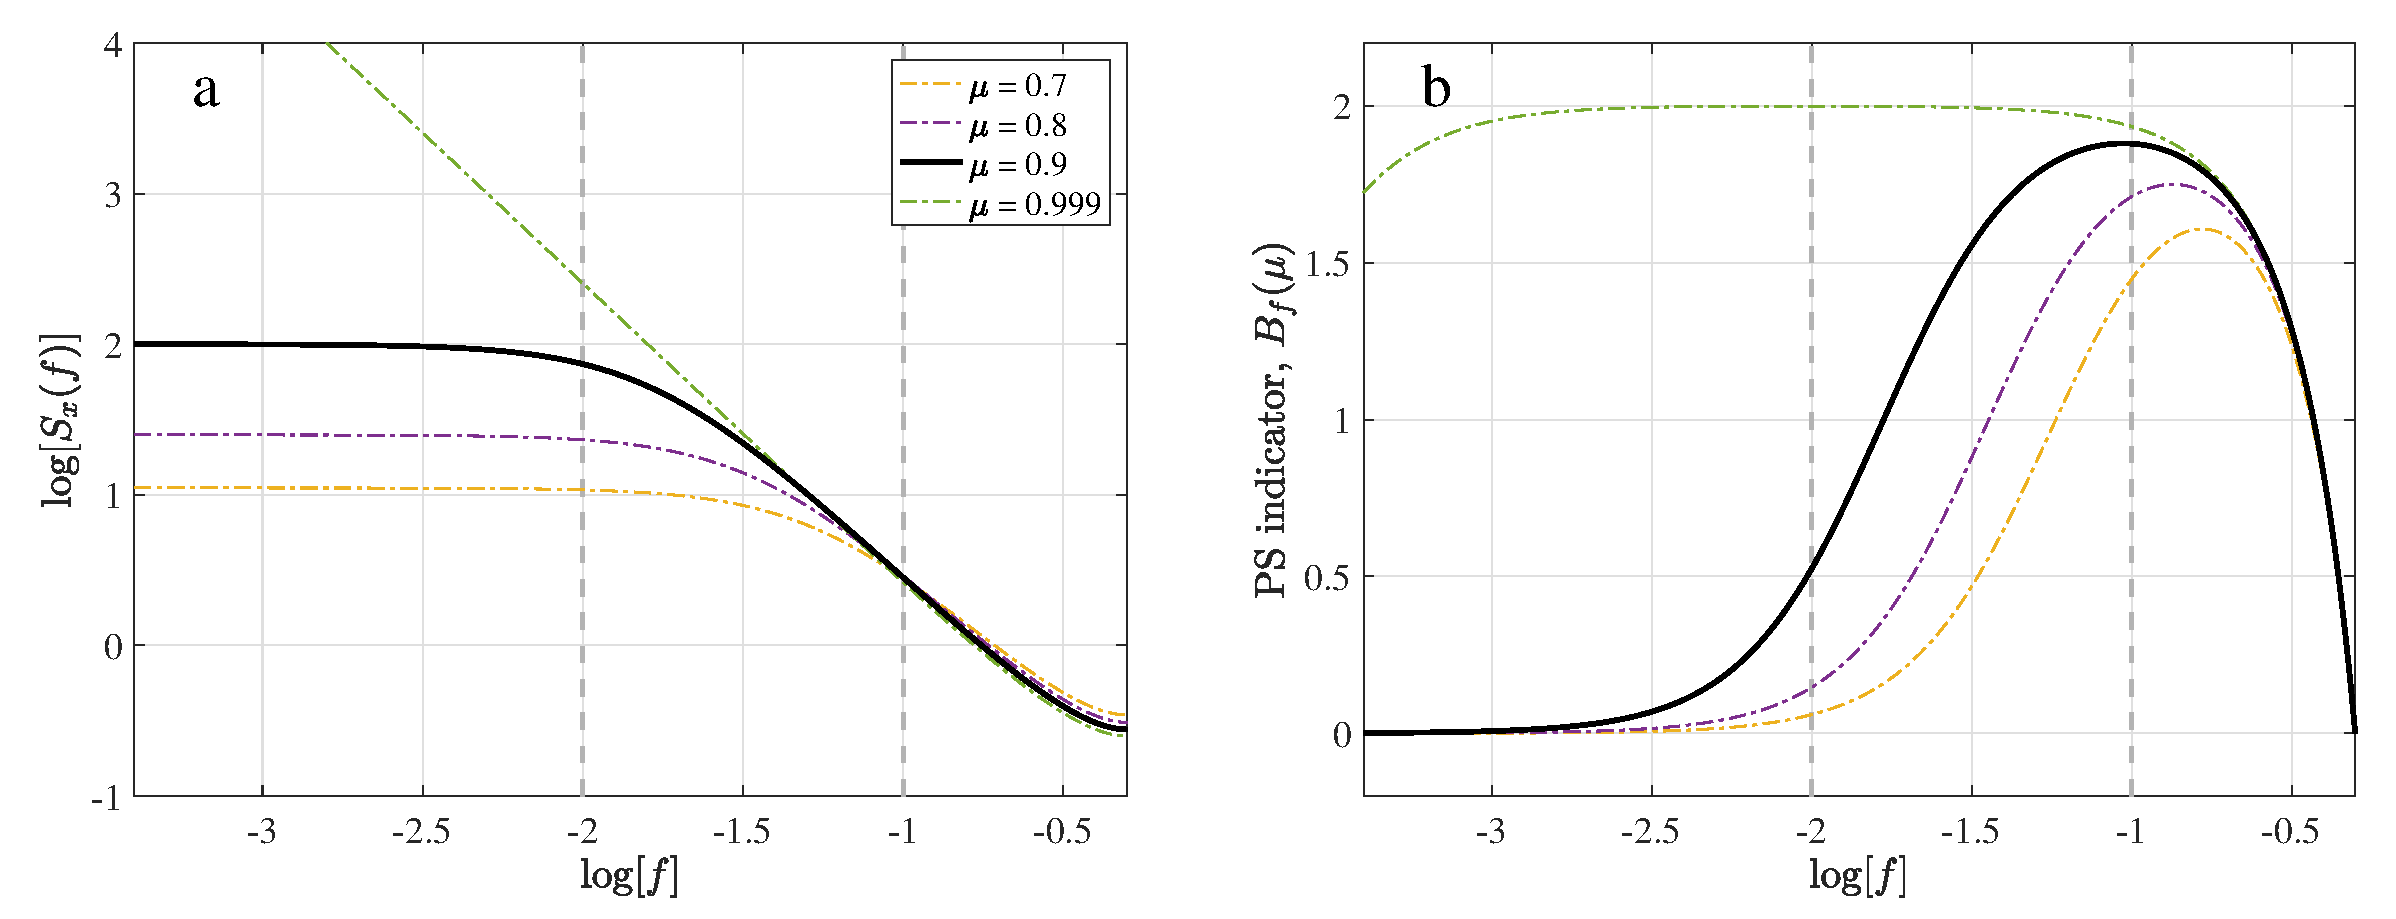
\includegraphics[width=0.9\linewidth]{AR1_powerspectrum}
	\caption{\Red{ Panel {\bf a}: The power spectrum of the AR(1) process (see equation~\ref{eqn:1D:AR1process_powerspectrum}) is plotted on a log-log scale for various values of the parameter $\mu$. Note the `white-noise' (flat) part of the power spectrum for small $f$ and the 'red-noise' (negative gradient) part for large $f$. Panel {\bf b}: The PS indicator (see equation~\ref{eqn:1D:AR1_psindicator}) is plotted as a function of $f$ for the same $\mu$ values. }}
	\label{fig:1D:AR1_powerspectrum}
\end{figure}

{\Red
In figure~\ref{fig:1D:AR1_powerspectrum} the power spectrum of the AR(1) process is plotted (panel {\bf a}) for parameter value $\mu = 0.9$. We note that for small values of $f$ ($\log f<\m2.5$) the ``white noise'' (flat) aspect of the power spectrum is visible whilst for larger values ($\log f\approx \m1$) we observe a ``red noise'' (gradient $= \m2$) feature, and there is a crossover which occurs at approximately $\log f= \m2$. We also note that, similar to the example in figure~\ref{fig:1D:crossover2}, this crossover point a value of $f$ dependent on the parameter $\mu$: also plotted are the power spectra for $\mu = 0.7,~ 0.8,~ 0.999$. In figure~\ref{fig:1D:AR1_powerspectrum}b the PS exponent $B_f$ is plotted as a function of $\log f$ for the same (fixed) values of $\mu$. We are able to see the white noise part of the power spectrum ($\log f<\m2.5$) where $B_f=0$ and the peak ($B_f\approx 2$), which occurs at $\log f\approx \m1$ for $\mu = 0.9$, corresponding to the negative-gradient `red noise' aspect of the power spectrum in panel {\bf a}. This plot also allows us to visualise the observation made in equation~\ref{eqn:1D:maximumPSindicator_AR1} that for large values of $f$ ($\log f > \m1$) the PS indicator does not reach a value close to the maximum value of 2, even for $\mu$ close to 1.

\begin{figure}
	\centering
	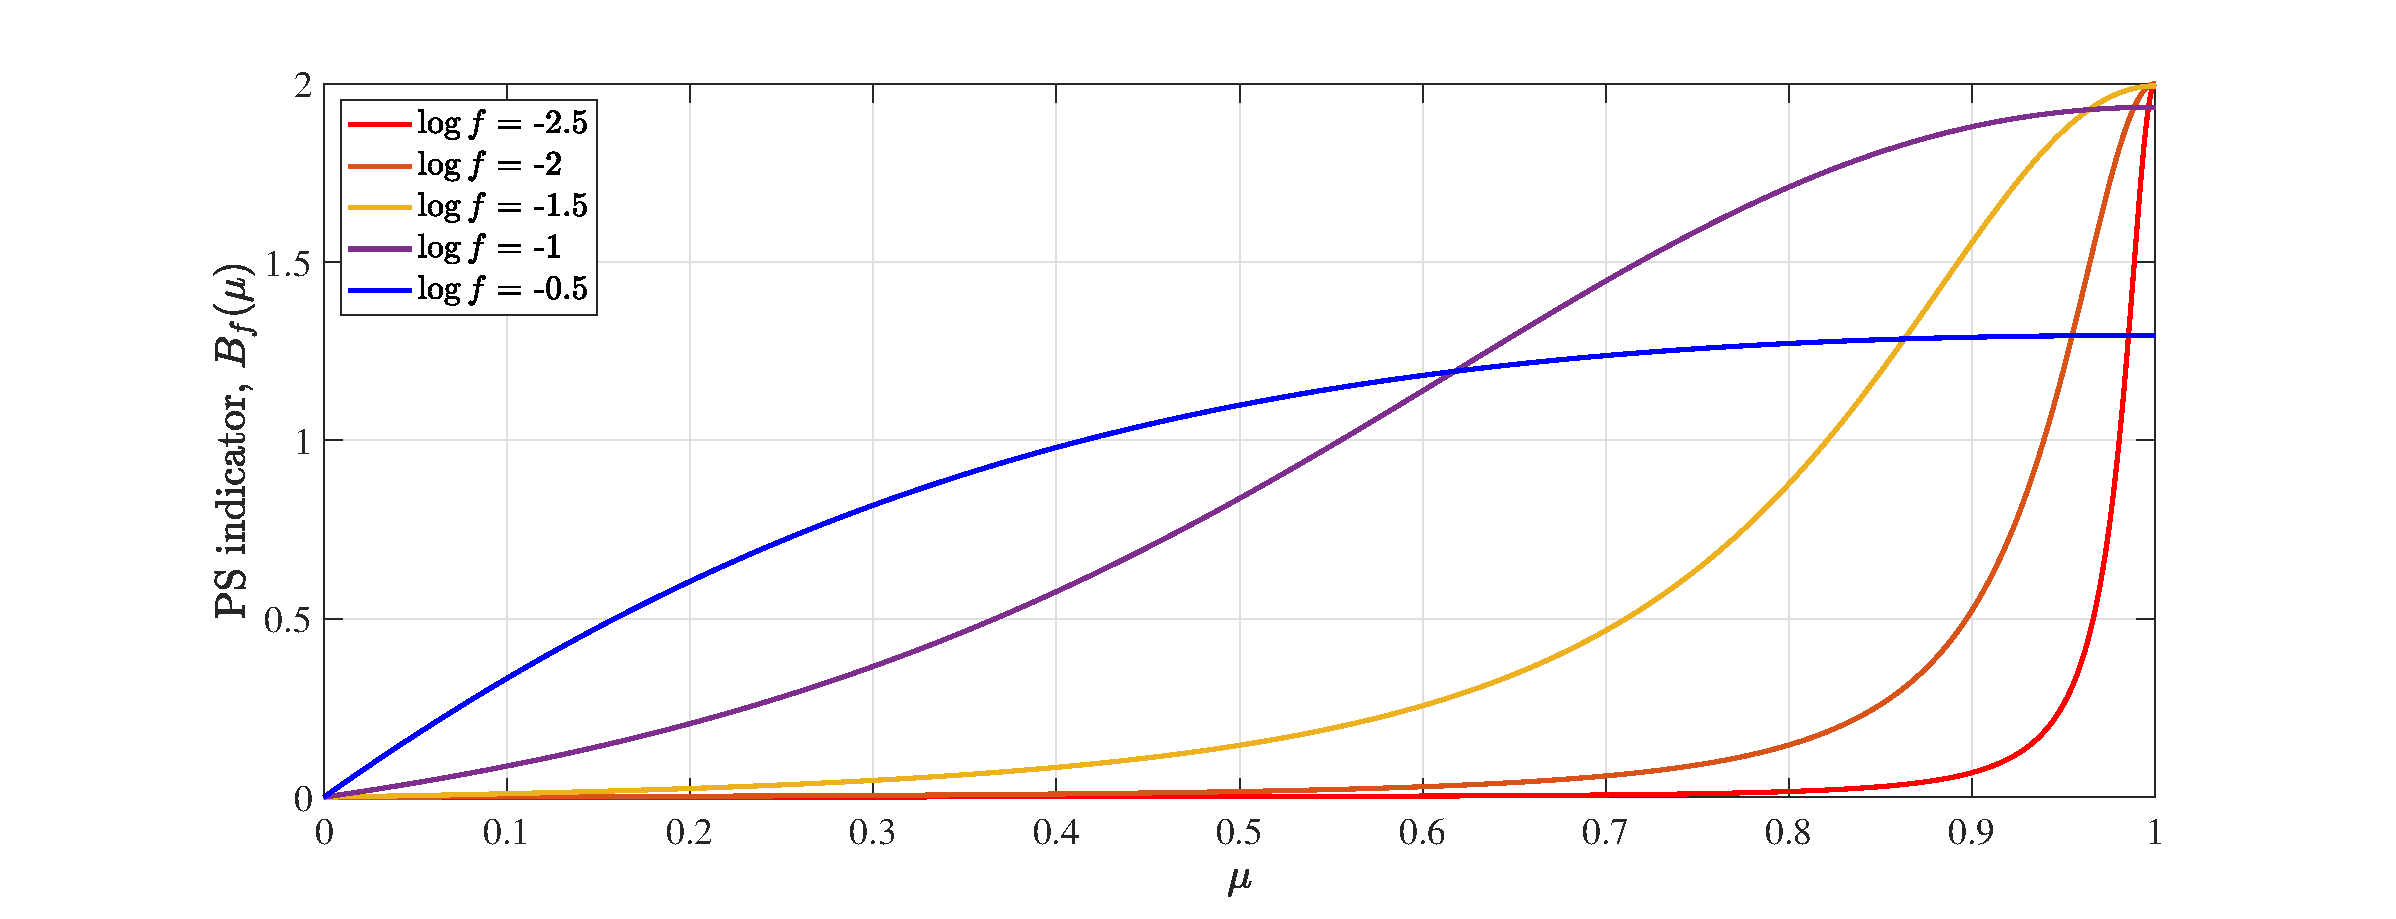
\includegraphics[width=\linewidth]{PSexponent_changingmu}
	\caption{ \Red{The PS indicator is plotted as a function of $\mu$ for various values of $f$. Note that for larger $f$ the PS indicator has a maximum value $<2$ while for smaller $f$ the indicator shows the characteristic increasing ('reddening') trend only in the $\mu>0.9$ range.}}
	\label{fig:1D:PSexponent_changingmu}
\end{figure}

In figure~\ref{fig:1D:PSexponent_changingmu} we plot the PS indicator (equation~\ref{eqn:1D:AR1_psindicator}) as a function of $\mu$ rather than as a function of time, which is equivalent to the assumption $\mu(t)=t$. The PS indicator increases, as expected, as $\mu$ increases from 0 to 1. We note that for very small values of $f$ ($\log f<\m2$) the indicator value is close to zero until the point $\mu=0.9$ when it increases very steeply. This effect can also been seen in figure~\ref{fig:1D:AR1_powerspectrum}b where we observe that even at $\mu=0.9$ the indicator is zero for small $f$, whereas for $\mu = 0.999$ the indicator is $\approx 2$ over the whole range $\m3<\log f<\m1$.  For larger $f$ it is possible to see the increasing trend in the indicator over the whole series of increasing $\mu$. For this reason, when one wishes to detect a `reddening' of noise due to critical slowing down, which is modelled as an AR(1) process \citep{ashwin2012}, the most obvious trend will be visible when measuring the PS scaling exponent using a frequency $\log f\geq\m2$. We note, however, that this will not be true if a relatively high base-level PS indicator ($B_f>0.5$) is observed for $\log f=\m2$, implying an AR(1) parameter $\mu>0.9$. In this case it may be more instructive to observe whether there is a steep increase in the indicator as $\mu$ increases between 0.9 and 1; this is clearly visible for $\log f=\m3$ but not for $\log f=\m1$. 

In practical applications where only short time series are available and the power spectrum is approximated by the fast Fourier transform periodogram, there may be very few data available in the lower frequencies due to the logarithmic scale. In these cases it may not be possible to reasonably estimate the PS exponent for small values of $f$ and so the frequencies used will be informed by the length of the time series. In table~\ref{tab:1D:AR1_frequencyrange} we have enumerated the number of data points in different frequency ranges having obtained the fast Fourier transform periodogram from a time series of $10^4$, $10^3$ and $10^2$ points. When using very short time series, say $100$ points, it is already impossible to estimate the gradient of the periodogram for frequencies $\log f<\m2$ because there are simply not enough data to perform a linear fit. However, in the range $\m2\leq\log f\leq\m1$ it is at least possible, with 10 points available, although we note that this will likely give a very noisy PS indicator and longer time series or large ensembles would be preferred.

\begin{table}
	\centering
	\begin{tabular}{ c c  c  c }
		\hline
		\multirow{2}{*}{Frequency range} & \multicolumn{3}{c}{Number of data in range}\\
		& $N=10^{4}$ & $N=10^{3}$ & $N=10^{2}$\\
		\hline \hline
		$\m3.5\leq\log f\leq\m2.5$ & 28   & 3   & 0\\
		$\m3\leq\log f\leq\m2$     & 91   & 10  & 1\\
		$\m2.5\leq\log f\leq\m1.5$ & 285  & 28  & 3\\
		$\m2\leq\log f\leq\m1$     & 901  & 91  & 10\\
		$\m1.5\leq\log f\leq\m0.5$ & 2846 & 285 & 28\\
		\hline
	\end{tabular}
	\caption{\Red{The fast Fourier transform periodogram is obtained for time series of length $10^4$, $10^3$ and $10^2$ and the number of data in various frequency ranges is recorded. For time series of length $10^2$ there are not sufficient data to estimate the PS scaling exponent for $\log f<\m2$.}}
	\label{tab:1D:AR1_frequencyrange}
\end{table}

Taking all of these factors into account, we conclude that using a frequency range $\m2\leq\log f\leq\m1$ in which to measure the PS scaling exponent will give the most clearly observable increase in the PS indicator during critical slowing down. At the higher end of this range we begin to observe the sudden drop in the maximum exponent value; at the lower end of the range there exist the dual problems of almost no increase for parameter values below $\mu=0.9$, and an insufficient number of data for estimation when dealing with short time series.

}


\subsection{Sensitivity of PS indicator to window size}
\label{subsec:1D:Exponents_as_EWS:PSsensitivity}
{\Red{
		In section~\ref{subsec:1D:Exponents_as_EWS:indicators}, where the PS indicator is introduced, we have remarked that by calculating the PS exponent $\beta$ of an AR(1) time series in the frequency range $\m1\leq\log_{10} f\leq\m2$ we can reconstruct the parameter $\mu$ of the AR(1) since the two are related via equation~\ref{eqn:1D:PSindicator:reconstruct_mu}, that is, 
		\begin{equation}
		\label{eqn:1D:PSindicator:reconstruct_mu_repro}
		\mu\approx b-\sqrt{b^2-1}~~~\text{where}~~~ b = \frac{\cos(0.2\pi)-10^\beta \cos(0.02\pi)}{1-10^\beta}.
		\end{equation}
		The numerical verification of this derived equation is presented in figure~\ref{fig:1D:PSofAR1} (page~\pageref{fig:1D:PSofAR1}), where we demonstrate that the analytic relationship between $\mu$	and $\beta$ is approximately the same as the relationship between the PS exponent and the lag-1 autocorrelation calculated for a set of AR(1) time series with parameter $\mu\in[0,1]$. This verification, however, used AR(1) time series of length $10^5$, and would only be a valid test of the PS indicator if a window size of $10^5$ were used. This is clearly not always possible in practical situations and, if it were, might anyway be computationally expensive. 
		
		The selection of the window size when calculating an EWS indicator in a sliding window is always a compromise which takes into account the nature of the time series data, the time scale of the tipping event to be detected or predicted, and the error in the EWS. A very short window size will typically contain more error in the indicator calculation, whilst a very large window size will smooth out the effect upon the indicator of the tipping event, or may be prevented by only a short time series being available for analysis. In order to investigate further the limitations of using a small window size, the numerical results presented in figure~\ref{fig:1D:PSofAR1} are examined in more detail here, this time using a range of different lengths of the AR(1) time series. 
		
		For a range of `series lengths' between $10^2$ and $10^5$, one hundred time series are produced from an AR(1) process with parameter in the range $0\leq\mu\leq1$. For each of these time series the value of $\mu$ is estimated using two different methods: by calculating the PS exponent and using the formula in equation~\ref{eqn:1D:PSindicator:reconstruct_mu_repro}, or simply by calculating the lag-1 autocorrelation (ACF1). In each case, the difference between this estimated value and the real value of $\mu$ is found simply as $|\mu-\mu_\text{est}|$ and the mean of these differences is taken over the $100$ values of $\mu$ to give a single-value measure of the error inherent in each method for each series length.
		
		In fact equation~\ref{eqn:1D:PSindicator:reconstruct_mu_repro} is only valid for $0<\mu\leq1$, or equivalently $0<\beta\leq1.985$. When estimating the parameter $\mu$ we therefore impose the piece-wise condition
		\begin{equation}
			\mu_\text{est} = \begin{cases}
			0&~\text{if}~\beta\leq0\\
			b-\sqrt{b^2-1}&~\text{if}~0<\beta\leq1.985\\
			1&~\text{if}~\beta>1.9850
			\end{cases}
		\end{equation}
		where $b$ is given as in equation~\ref{eqn:1D:PSindicator:reconstruct_mu_repro}. In applications of the PS indicator to tipping points we are interested in the value of the PS indicator itself as a proxy for `reddening' noise in a time series and we do not literally estimate the AR(1) model parameter in this way. For the purpose of comparison, however, this is a useful exercise. 
		
		The results of this exercise are presented in figure~\ref{fig:1D:PSsensitivity}a whilst the individual results for the time series of length $10^2$ (the shortest considered) and length $10^5$ (the longest considered) are shown in figures figure~\ref{fig:1D:PSsensitivity}b,c. We note (in panel {\bf a}) that the error is always larger in the power spectrum approach than in the autocorrelation approach and that whilst the error in each method is larger for short series lengths, so the difference between the two methods is also larger. 
	}}



\begin{figure}
	% plotted using the Matlab script 'PSwindowsize_sensitivity.m'
	\centering
	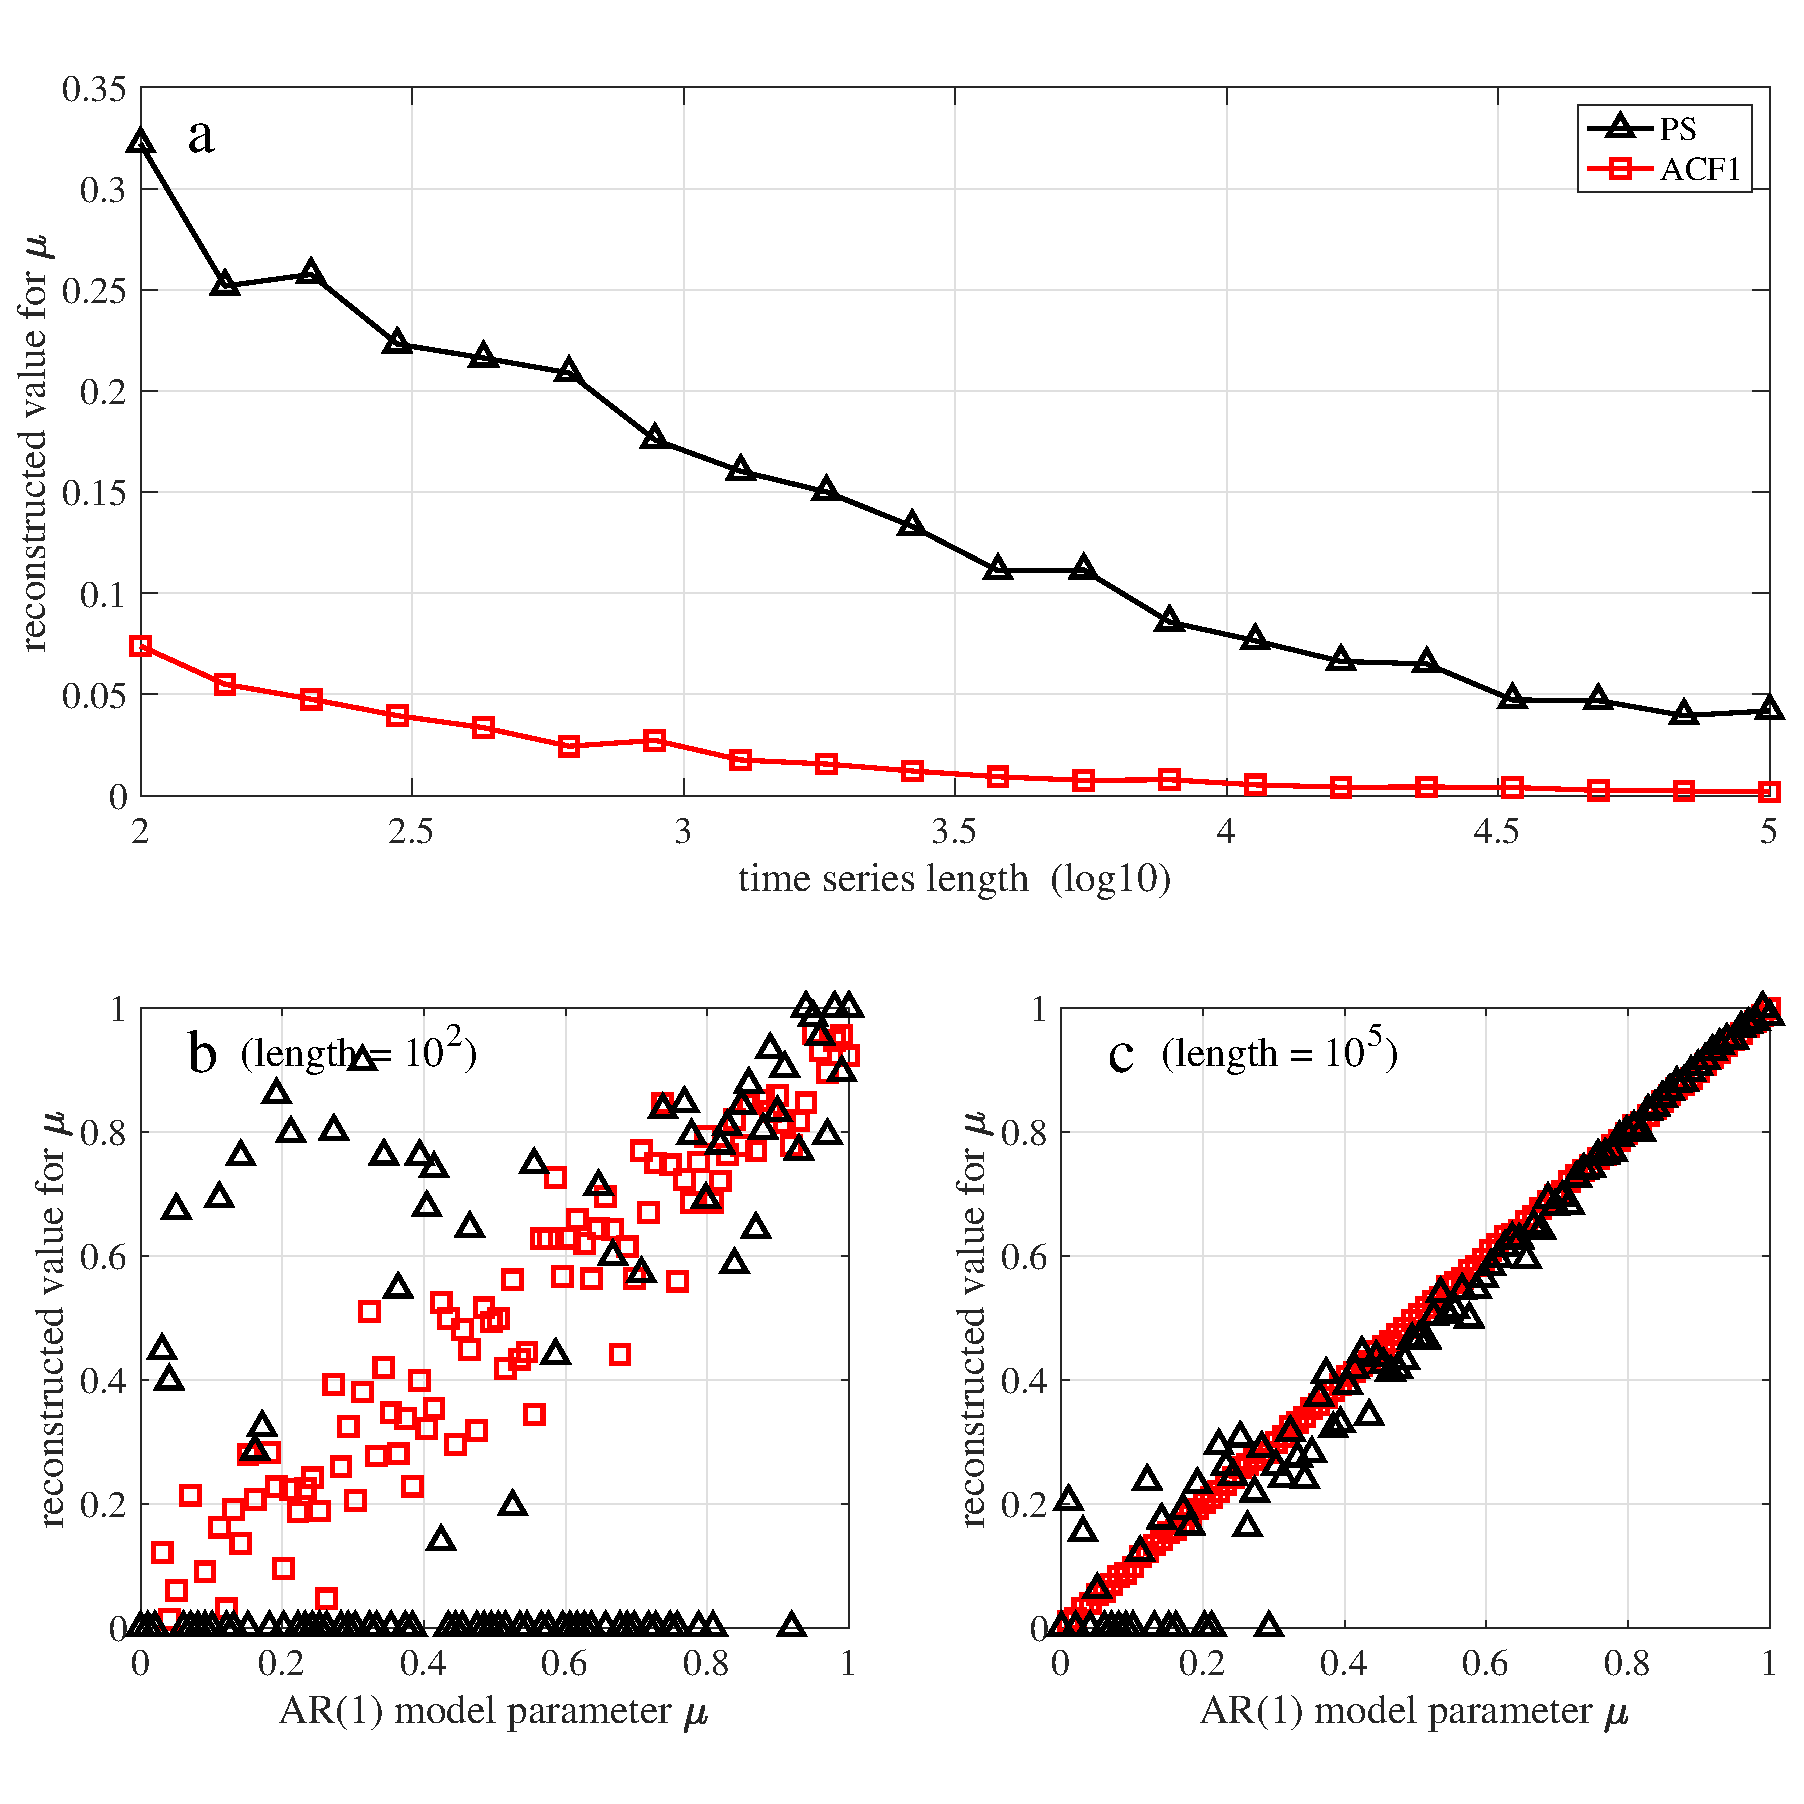
\includegraphics[width=0.9\linewidth]{PSwindowsize_sensitivity_1e5}
	\caption{\label{fig:1D:PSsensitivity}
		\Red{Panel {\bf a}: For $10^2\leq N\leq 10^5$ time series of length $N$ are created using an AR(1) model with $100$ different values of the parameter $\mu$ in the range $[0,1]$. The value of the model parameter is then estimated using either the lag-1 autocorrelation or the PS exponent $\beta$ (see equation~\ref{eqn:1D:PSindicator:reconstruct_mu_repro}). The mean difference between the estimated value and the true value is plotted for the ACF1 method (red squares) and the PS method (black triangles).  Panels {\bf b}, {\bf c}: The estimated values of the parameter $\mu_{\text{est}}$ are plotted against the true values $\mu$ when using a series length $N=10^2$ (the shortest considered) and $10^5$ (the longest considered). }
	}
\end{figure}

{\Red{
		Whilst it is clear that the ACF1 method out-performs the PS method for every time series length, we note that in both the short series (length $N=10^2$) and the long series (length $N=10^5$) the PS method is better at estimating the true value of $\mu$ for higher values of $\mu$ than it is for lower values. In figure~\ref{fig:1D:PSsensitivity}b ($N=10^2$) we note that whilst the estimated value is extremely variable for low values of $\mu$ it is reasonably close to the true value for $\mu>0.8$. In figure~\ref{fig:1D:PSsensitivity2} we replot the same data as figure~\ref{fig:1D:PSsensitivity}a, but only considering either small values $\mu\leq0.4$ (top panel) or large values $\mu\geq0.6$ (bottom panel). We note the improved accuracy of the PS method when considering only large values of $\mu$, particularly for series length $N>10^3$. This is to be expected somewhat if we consider the shape of the function that relates $\mu$ and $\beta$ which has been used in this experiment. The value of $\beta$ as a function of $\mu$ is shown in figure~\ref{fig:1D:PSofAR1}, the formula given by equation~\ref{eqn:1D:PSindicator:reconstruct_mu_repro} is simply the inverse function. We see in this that for small $\mu$ a large change in $\mu$ gives only a small change in $\beta$, whereas this is the opposite for large $\mu$. We can therefore expect that, when $\mu$ is small, a small error in the estimation of the PS exponent $\beta$ will translate into a much larger error in the estimated value of $\mu$ using the formula in equation~\ref{eqn:1D:PSindicator:reconstruct_mu_repro}. When using the PS indicator we bear in mind that it is used as a proxy for the `reddening' of noise over time which is caused by critical slowing down, not to provide an accurate parametrisation of an AR(1) model. Also, the increase in the AR(1) parameter which is expected in the presence of critical slowing down is not necessarily linear, and so the non-linear relationship between $\mu$ and $\beta$ (which is here responsible for the error at low values of $\mu$) may not necessarily be a problem, depending on the application.
}}

\begin{figure}
	% plotted using the Matlab script 'PSwindowsize_sensitivity.m'
	\centering
	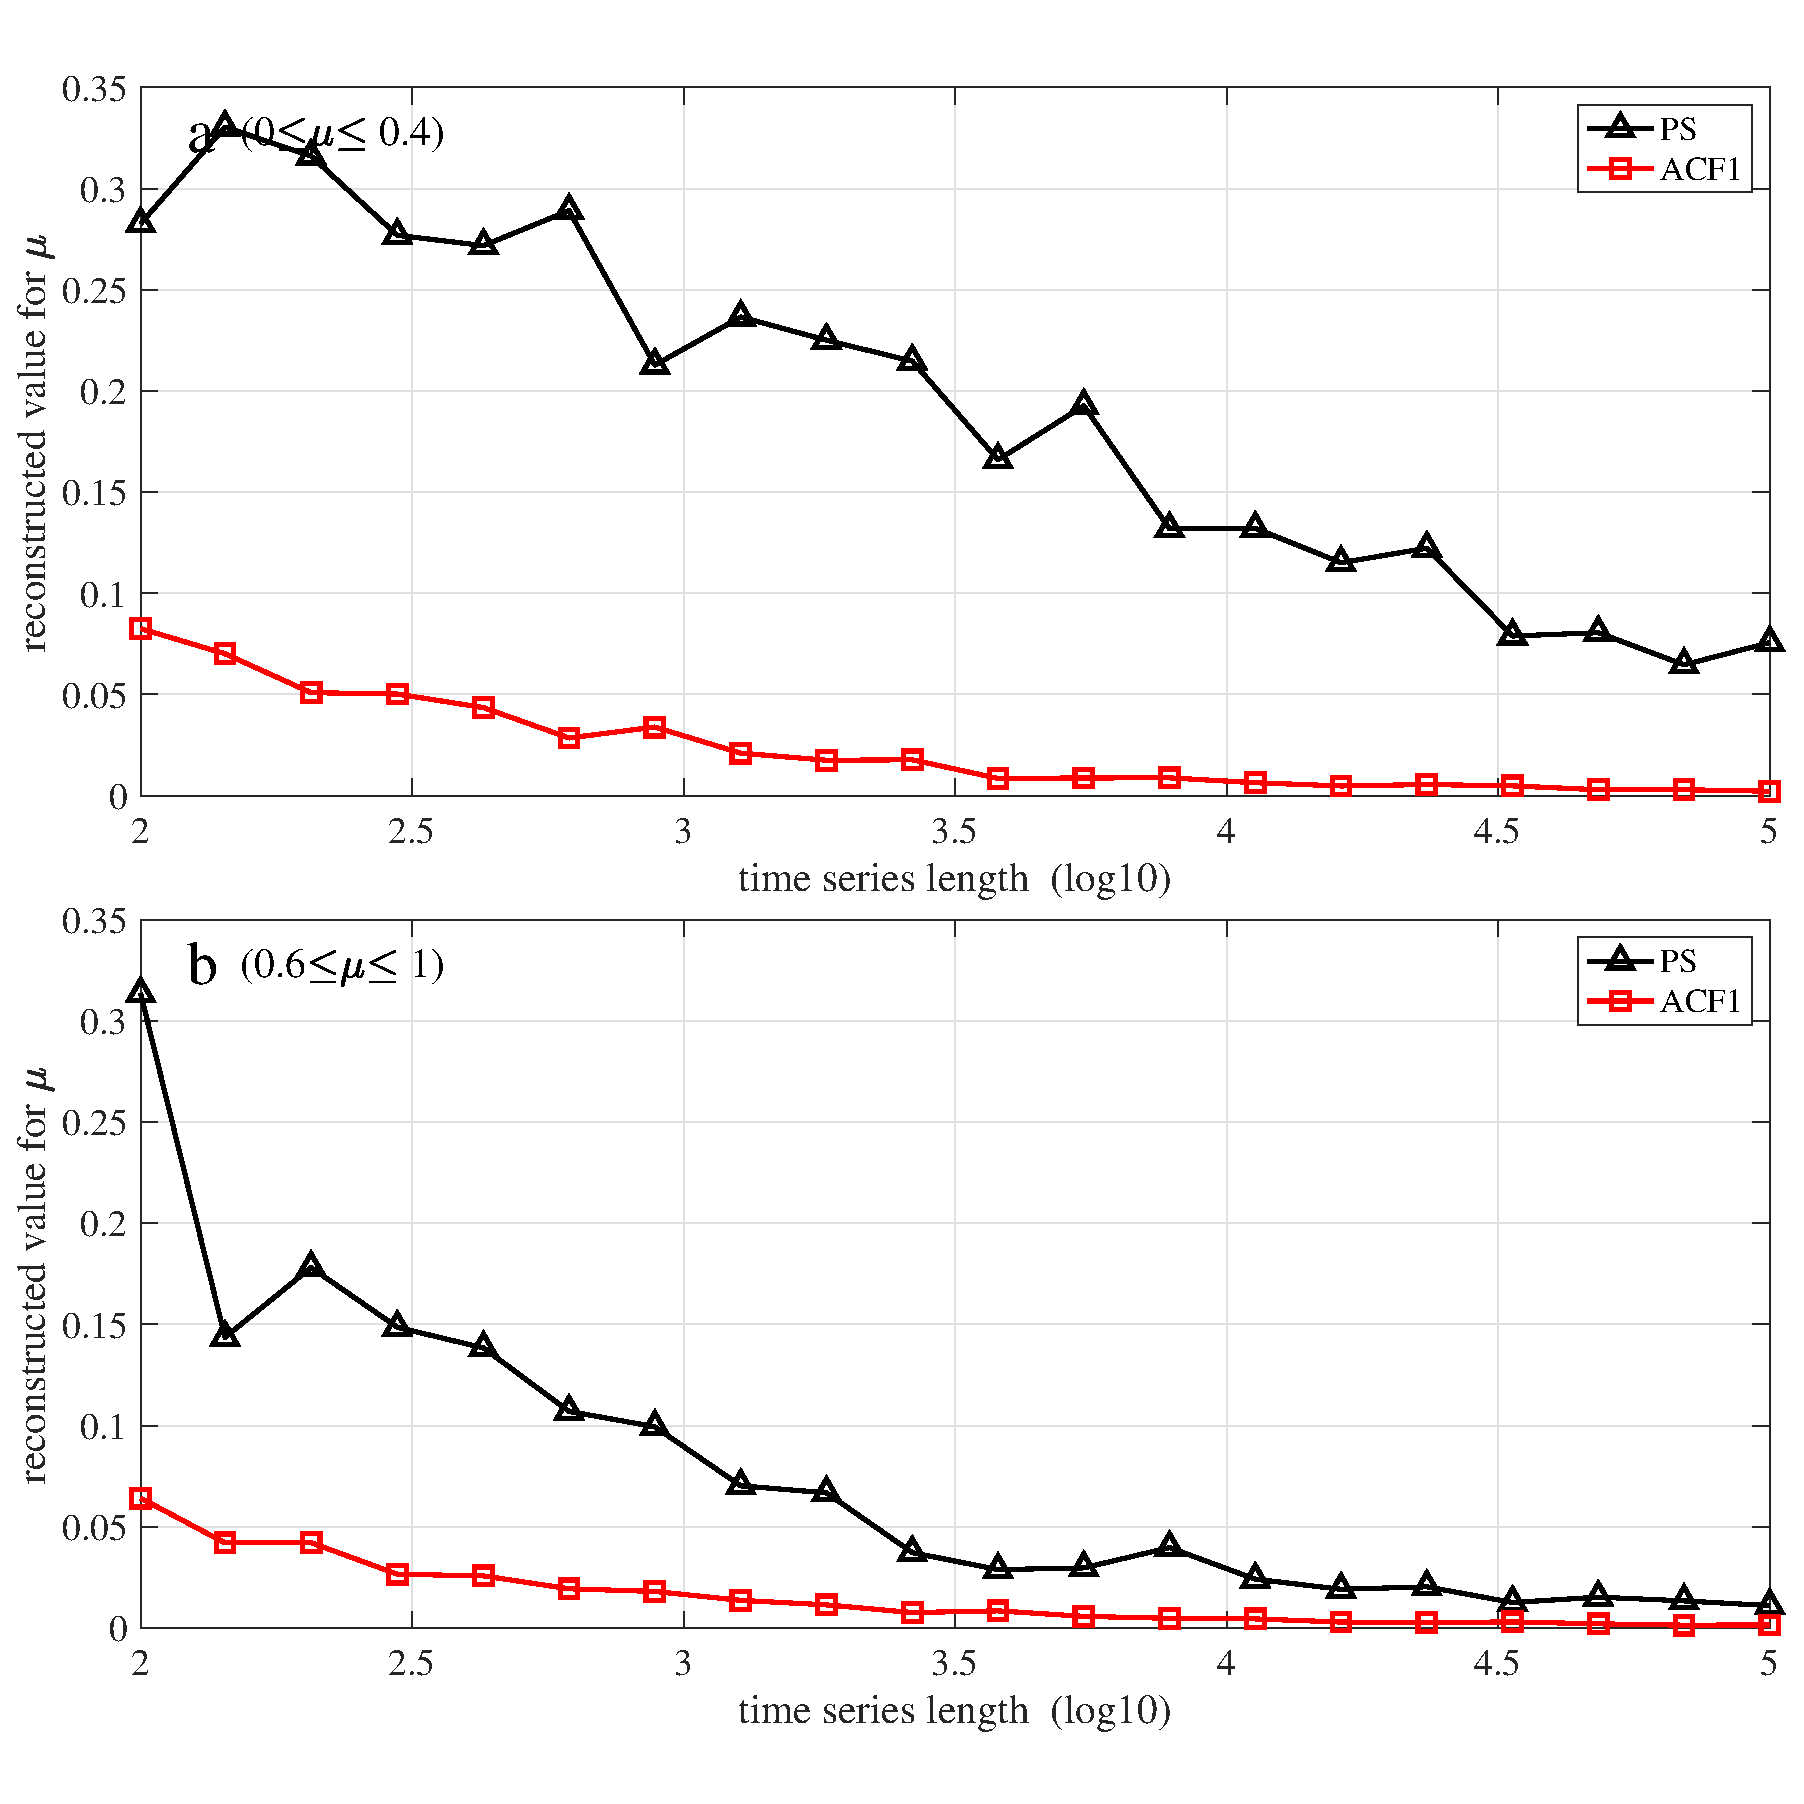
\includegraphics[width=0.9\linewidth]{PSwindowsize_sensitivity_BigAndSmall_1e5}
	\caption{\label{fig:1D:PSsensitivity2}
		\Red{For $10^2\leq N\leq 10^5$ time series of length $N$ are created using an AR(1) model with $100$ different values of the parameter $\mu$. The value of the model parameter is then estimated using either the lag-1 autocorrelation or the PS exponent $\beta$ (see equation~\ref{eqn:1D:PSindicator:reconstruct_mu_repro}). The mean difference between the estimated value and the true value is plotted for the ACF1 method (red squares) and the PS method (black triangles). Panel {\bf a} shows the result of the experiment for $\mu$ in the range $[0, 0.4]$ (small $\mu$) whilst panel {\bf b} shows the result of the experiment for $\mu$ in the range $[0.6, 1]$ (large $\mu$). }
	}
\end{figure}

{\Red{
		In figure~\ref{fig:1D:PSsensitivity_trend} we show the results of this experiment repeated but instead of a simple AR(1) model, a parabolic trend has been superimposed onto the resulting times series. For each different value of the series length $N$, a time series is produced using
		\begin{equation}
			X(t_{n}) = \mu X(t_{n-1}) + \eta_n + 5t_n^2\,,
		\end{equation} 
		where $[t_1,\dots,t_N] = [0,\dots,1]$ and the $\eta_n$ are independent Gaussian white noise terms. We expect that by introducing non-stationarity in this way the auto-correlation of the time series will increase and tend to make any estimate of the parameter $\mu$ an \emph{over}-estimate. In figure~\ref{fig:1D:PSsensitivity_trend}b we see that this is indeed the case where the series length is $N=10^2$: both estimated parameters are much closer to $1$ than to the true value, although the estimate obtained from the PS method (black triangles) appears to be random whilst the values obtained using the ACF1 method follow a linear pattern, whilst being consistently higher than the true values. For longer series lengths, however, this is not the case. In figure~\ref{fig:1D:PSsensitivity_trend}c, where the series length is $N=10^5$, the estimated values obtained using ACF1 follow the same linear relationship to the true values as they did for smaller $N$. The values obtained using the PS method are, however, in agreement with the true values, especially closely for the larger values of $\mu$. It appears that estimating the AR(1) model parameter using the PS exponent is not affected by whether there is or is not a trend superimposed on the AR(1) process time series, at least when the time series is sufficiently long. 
		
		In the context of providing early warning signals it is, of course, not the value of the indicator that is important but the trend in the indicator over time. In light of this, it is not necessarily a problem that the ACF1 indicator is biased by the trend in the time series, but in cases where trends in the time series are not predictable this bias could cause misleading trends to appear in the ACF1 indicator series. This bias may be overcome by first detrending each segment of the time series in which the indicator value is calculated, which is similar in principle to the detrending step in the DFA algorithm \citep{kantelhardt2001, livina2007}. For long time series, or long window sizes, the PS indicator calculation may provide the benefit of not requiring the detrending step, which may in fact introduce new inaccuracies if the detrending is of the wrong order. 
				
	}}

\begin{figure}
	% plotted using the Matlab script 'PSwindowsize_sensitivity.m'
	\centering
	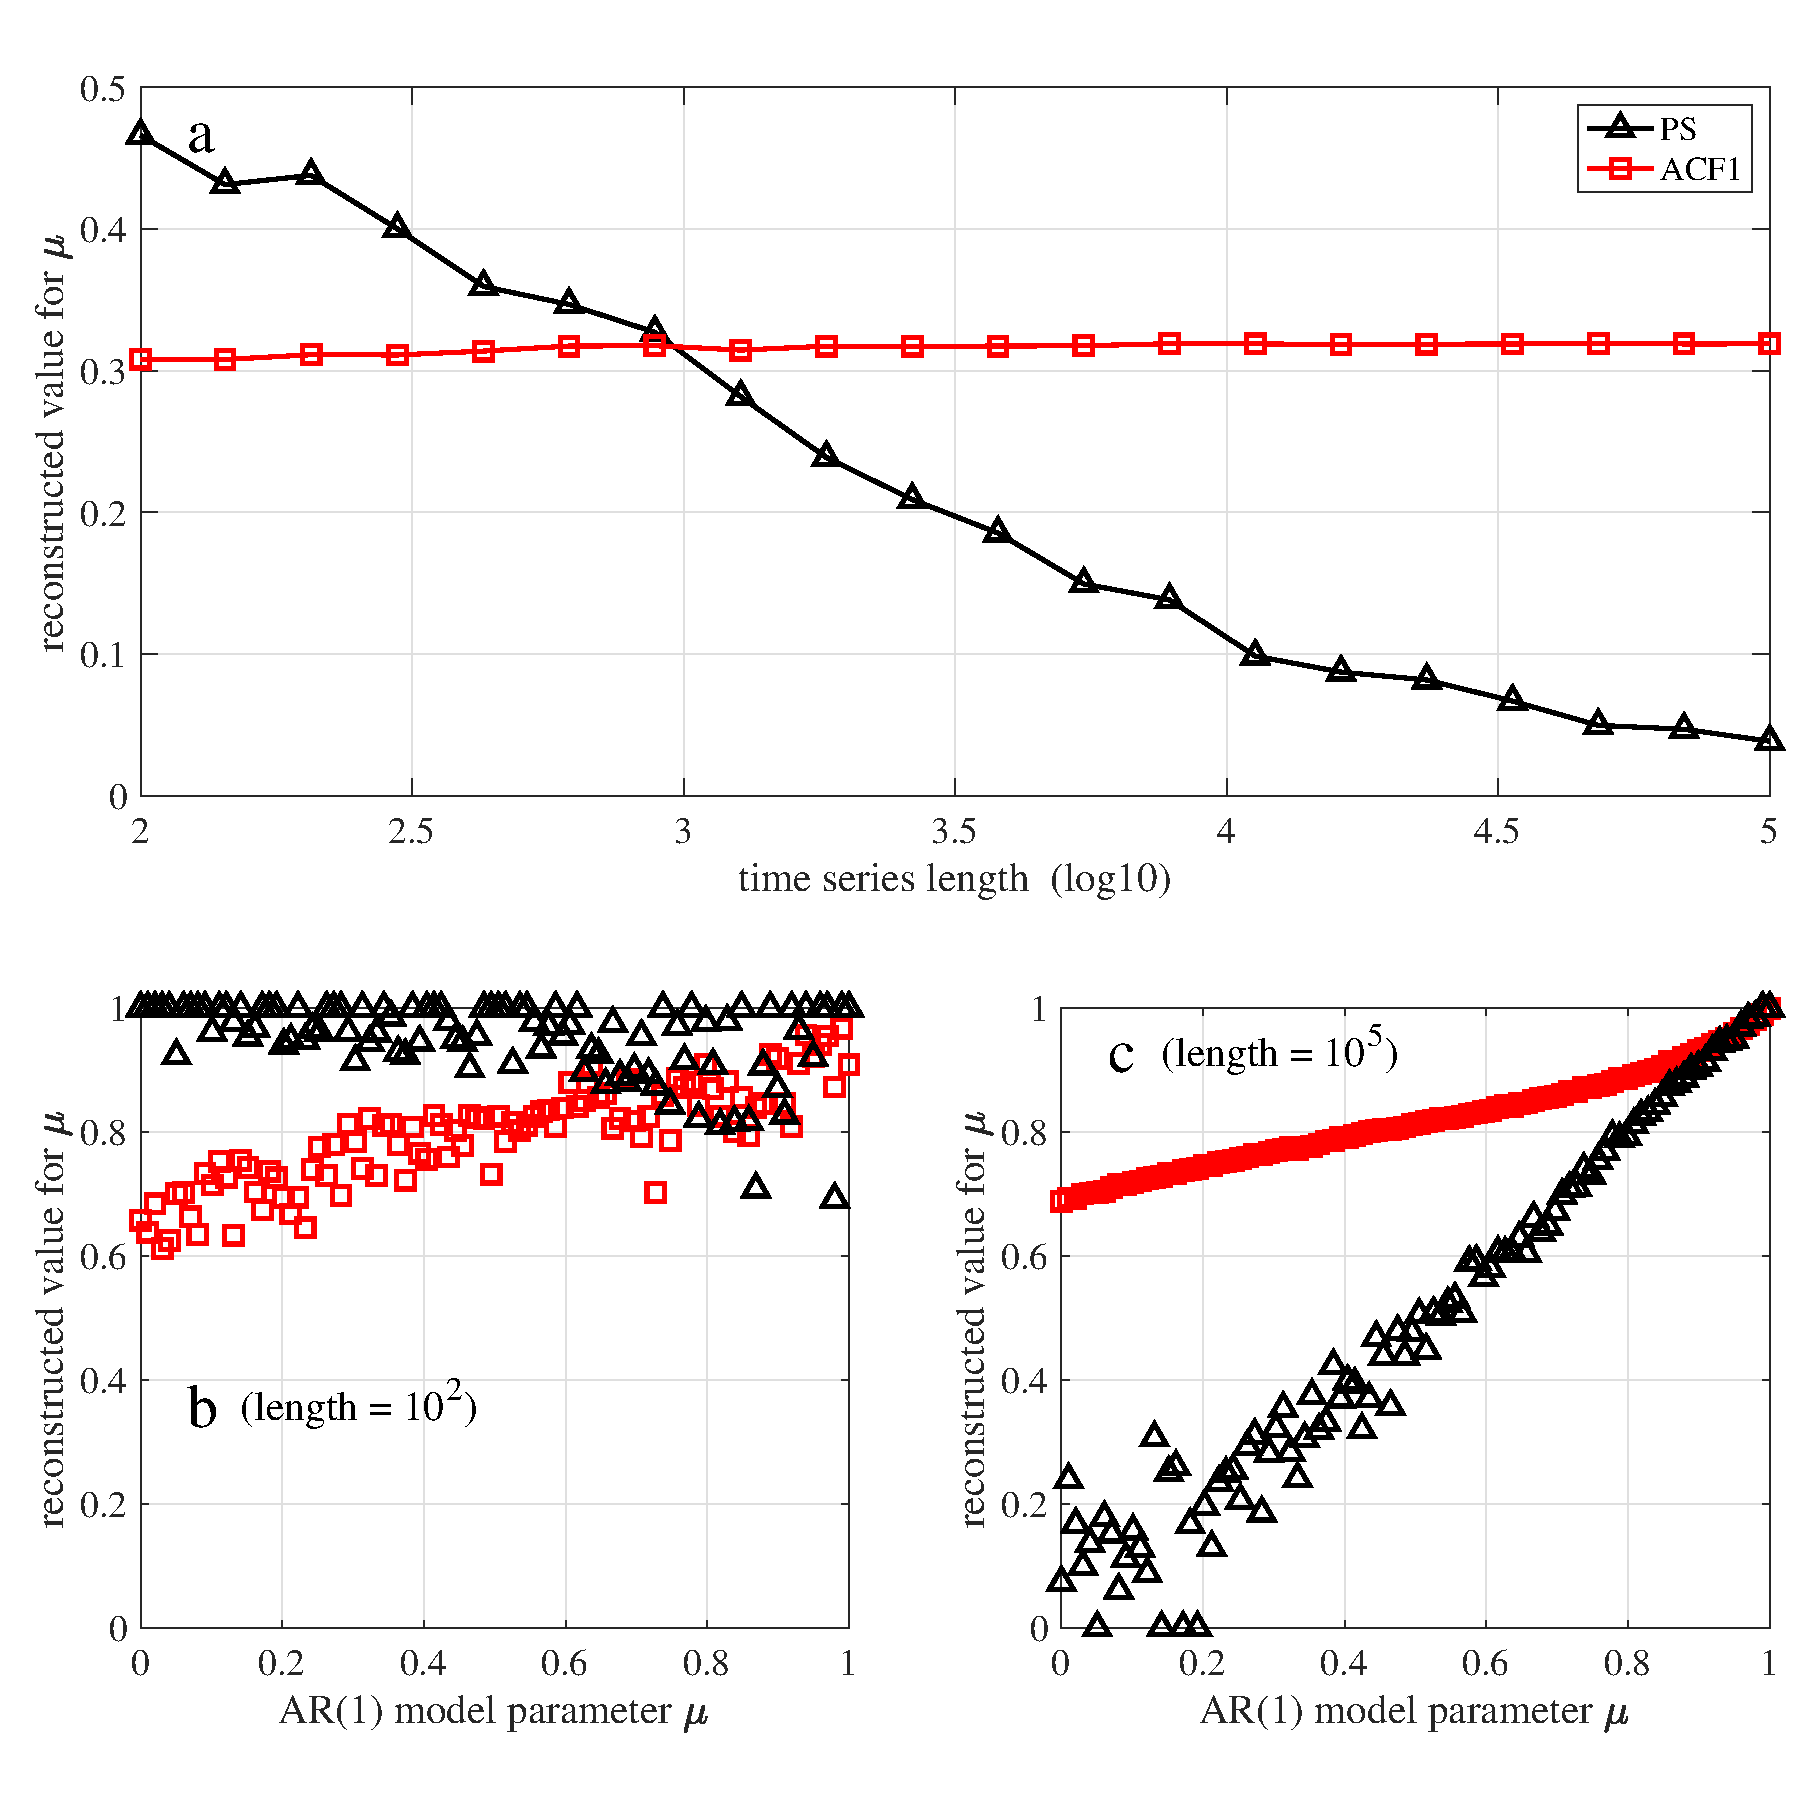
\includegraphics[width=0.9\linewidth]{PSwindowsize_sensitivity_trend}
	\caption{\label{fig:1D:PSsensitivity_trend}
		\Red{[Repeat of the experiment in figure~\ref{fig:1D:PSsensitivity} but the AR(1) model has a superimposed parabolic trend] Panel {\bf a}: For $10^2\leq N\leq 10^5$ time series of length $N$ are created using an AR(1) model with a parabolic trend with $100$ different values of the parameter $\mu$ in the range $[0,1]$. The value of the model parameter is then estimated using either the lag-1 autocorrelation or the PS exponent $\beta$ (see equation~\ref{eqn:1D:PSindicator:reconstruct_mu_repro}). The mean difference between the estimated value and the true value is plotted for the ACF1 method (red squares) and the PS method (black triangles).  Panels {\bf b}, {\bf c}: The estimated values of the parameter $\mu_{\text{est}}$ are plotted against the true values $\mu$ when using a series length $N=10^2$ (the shortest considered) and $10^5$ (the longest considered). }
	}
\end{figure}

\subsection{Parametrising an AR(1) process with non-constant parameter}
\label{subsec:1D:Exponents_as_EWS:PSnonstationary}
{\Red{
		All of the results in section~\ref{subsec:1D:Exponents_as_EWS:PSsensitivity} use time series from an AR(1) process $x(t_n) = \mu x(t_{n-1})+\eta_n$ where $\mu$ is constant. Indeed, the work in section~\ref{subsec:1D:Exponents_as_EWS:determining_frequency_range}, where we determine the frequency range in which to estimate the PS exponent assumes a constant $\mu$ and relies on the equation for the power spectrum of such an AR(1) process (see equation~\ref{eqn:1D:PSindicator:AR1powerspectrum}, page~\pageref{eqn:1D:PSindicator:AR1powerspectrum}). Of course, in applications of the PS indicator, or any indicator, to obtain an early warning signal, such stationarity cannot be assumed. Indeed, the very purpose of using these indicators is to detect an \emph{increase} in the `redness' due to critical slowing down, for which the AR(1) parametrisation is a proxy. 
		
		In practice we apply the early warning indicators to time series of dynamical systems with constantly changing parameters, and therefore within each time window the parameters will also be changing. In this case the PS scaling exponent or the lag-1 autocorrelation is calculated for this window of the time series and the result is provide a single-value measure representing the shape of the power spectrum in that window. Taking the single-parameter AR(1) model as an example, we might desire that the estimated value $\mu_\text{est}$ obtained using these methods is equal to the mean value of parameter $\mu$ in that window, which would produce consistent results if the rate of change of $\mu$ was non-constant. 
		
		We consider a modified AR(1) process
		\begin{equation}
			\label{eqn:1D:AR1process_changingparameter}
			x(t_n) = \mu_n x(t_{n-1})+\eta_n
		\end{equation}
		where the $\mu_n$ increase linearly in some interval $[\mu_0, \mu_N]$. If we calculate the PS exponent or lag-1 autocorrelation of this process we desire that the result is the same as it would be for a normal AR(1) process with constant parameter $\mu=(\mu_0+\mu_N)/2$ the mean value of the changing parameter. We test this hypothesis experimentally by partitioning the interval $[0,1]$ into $30$ overlapping segments of length $0.2$, so that the first segment is the interval $[0,0.2]$, etc.. For each segment we construct a length $N=10^5$ time series of an AR(1) process with $\mu$ increasing, as in equation~\ref{eqn:1D:AR1process_changingparameter}, within the interval defined by that segment. The PS exponent $\beta$ is then calculated for that time series, as is the lag-1 autocorrelation. 
		
		The results of this experiment are shown in figure~\ref{fig:1D:PS_nonstationary}. The intervals over which $\mu$ increases in each time series is plotted as a horizontal line, with the midpoint marked by a circle. The grey line shows the expected relationship between an AR(1) parameter and either the PS exponent (panel {\bf a}) or the lag-1 autocorrelation (panel {\bf b}). We note that in both cases the midpoint of the interval is close to the value that would be expected if using a constant-parameter AR(1) process with that midpoint as the parameter. We are able to conclude then that for the modified AR(1) process of equation~\ref{eqn:1D:AR1process_changingparameter}, when $\mu$ is increasing linearly, the PS indicator and ACF1 indicator can be expected to provide consistent results. 
		
		In figure~\ref{fig:1D:PS_nonstationary_BigMu} we look more closely at this effect for only values of $\mu$ greater than $0.6$, this time using a segment size of $0.1$ rather than $0.2$, and we note that the results are much the same, although the difference between the calculated value at the midpoints (circles) and the true values (grey line) is less both for the PS exponent and the lag-1 ACF. This is to be expected since the segments are shorter and so the parameter varies less over each time series, and also we know the PS exponent estimation to be more accurate for larger values of the AR(1) parameter (see section~\ref{subsec:1D:Exponents_as_EWS:PSsensitivity}).

}}

\begin{figure}
	% plotted using the Matlab script 'PS_nonstationary.m'
	\centering
	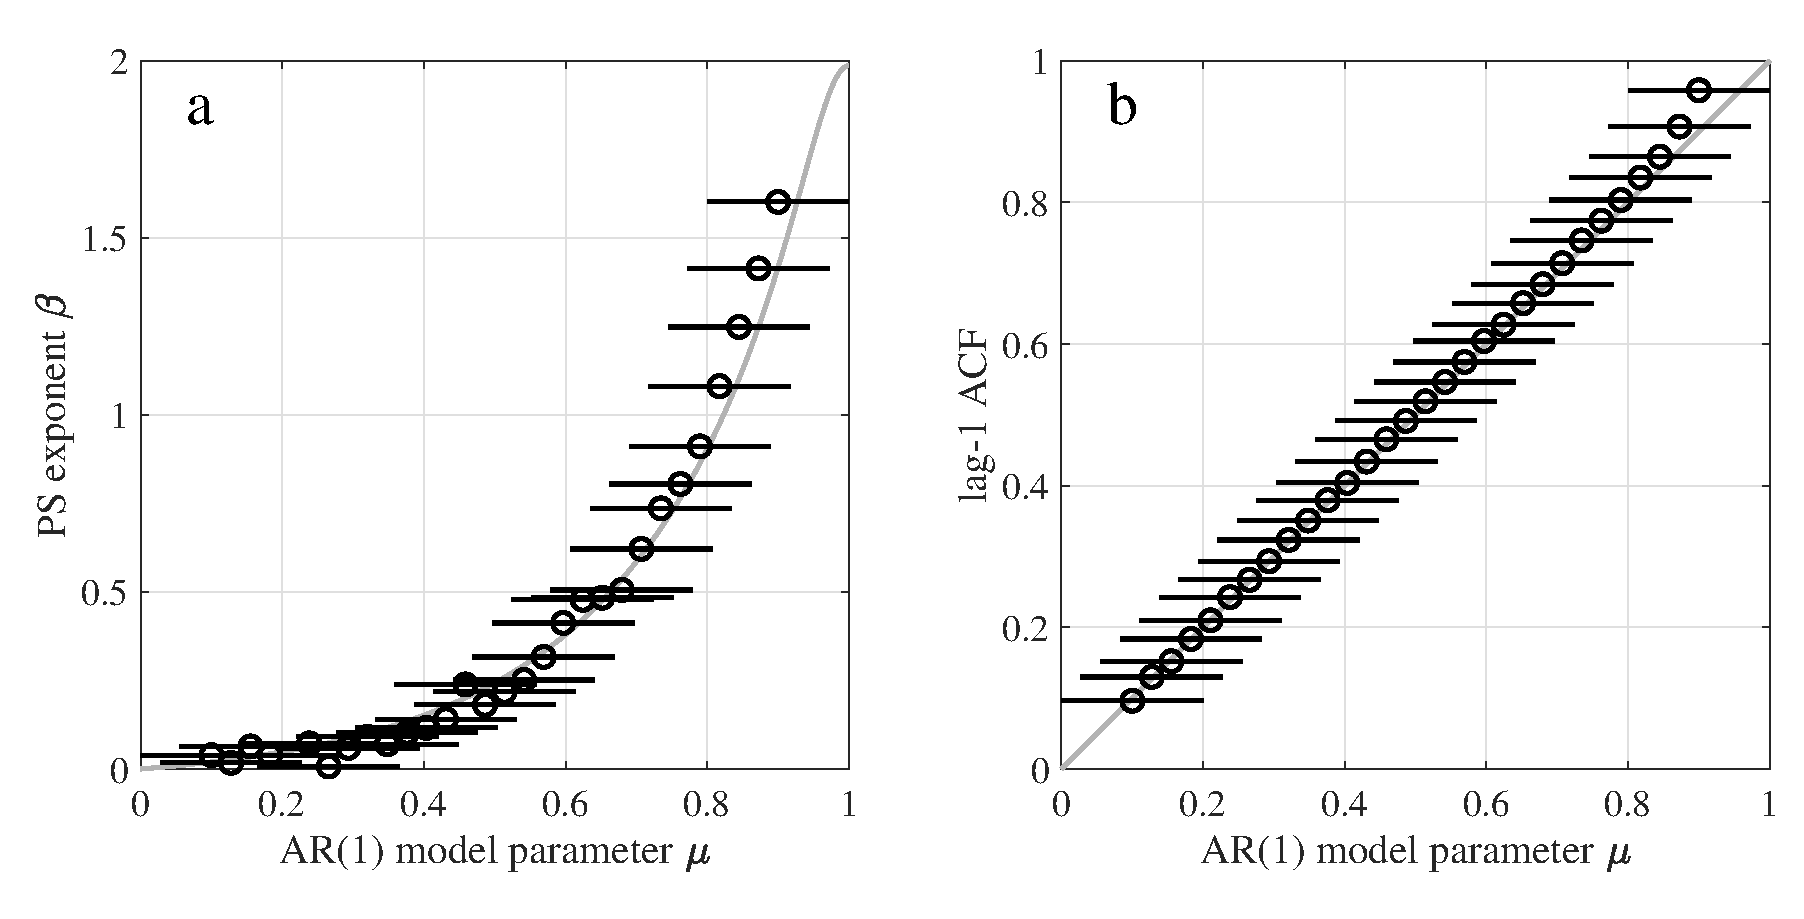
\includegraphics[width=0.9\linewidth]{PS_nonstationary}
	\caption{\label{fig:1D:PS_nonstationary}
		\Red{ $30$ time series of length $10^5$ are produced from an AR(1) process with parameter $\mu$ increasing linearly within an interval of values of length $0.2$. The PS exponent (panel {\bf a}) and the lag-1 ACF (panel {\bf b}) are calculated for each time series and the interval of $\mu$ values is plotted against the result in each case. The midpoints of the intervals are marked by circles. A grey line shows, in each case, the true value of $\beta$ or the lag-1 ACF for an AR(1) process with parameter $\mu$.}
	}
\end{figure}

\begin{figure}
	% plotted using the Matlab script 'PS_nonstationary.m'
	\centering
	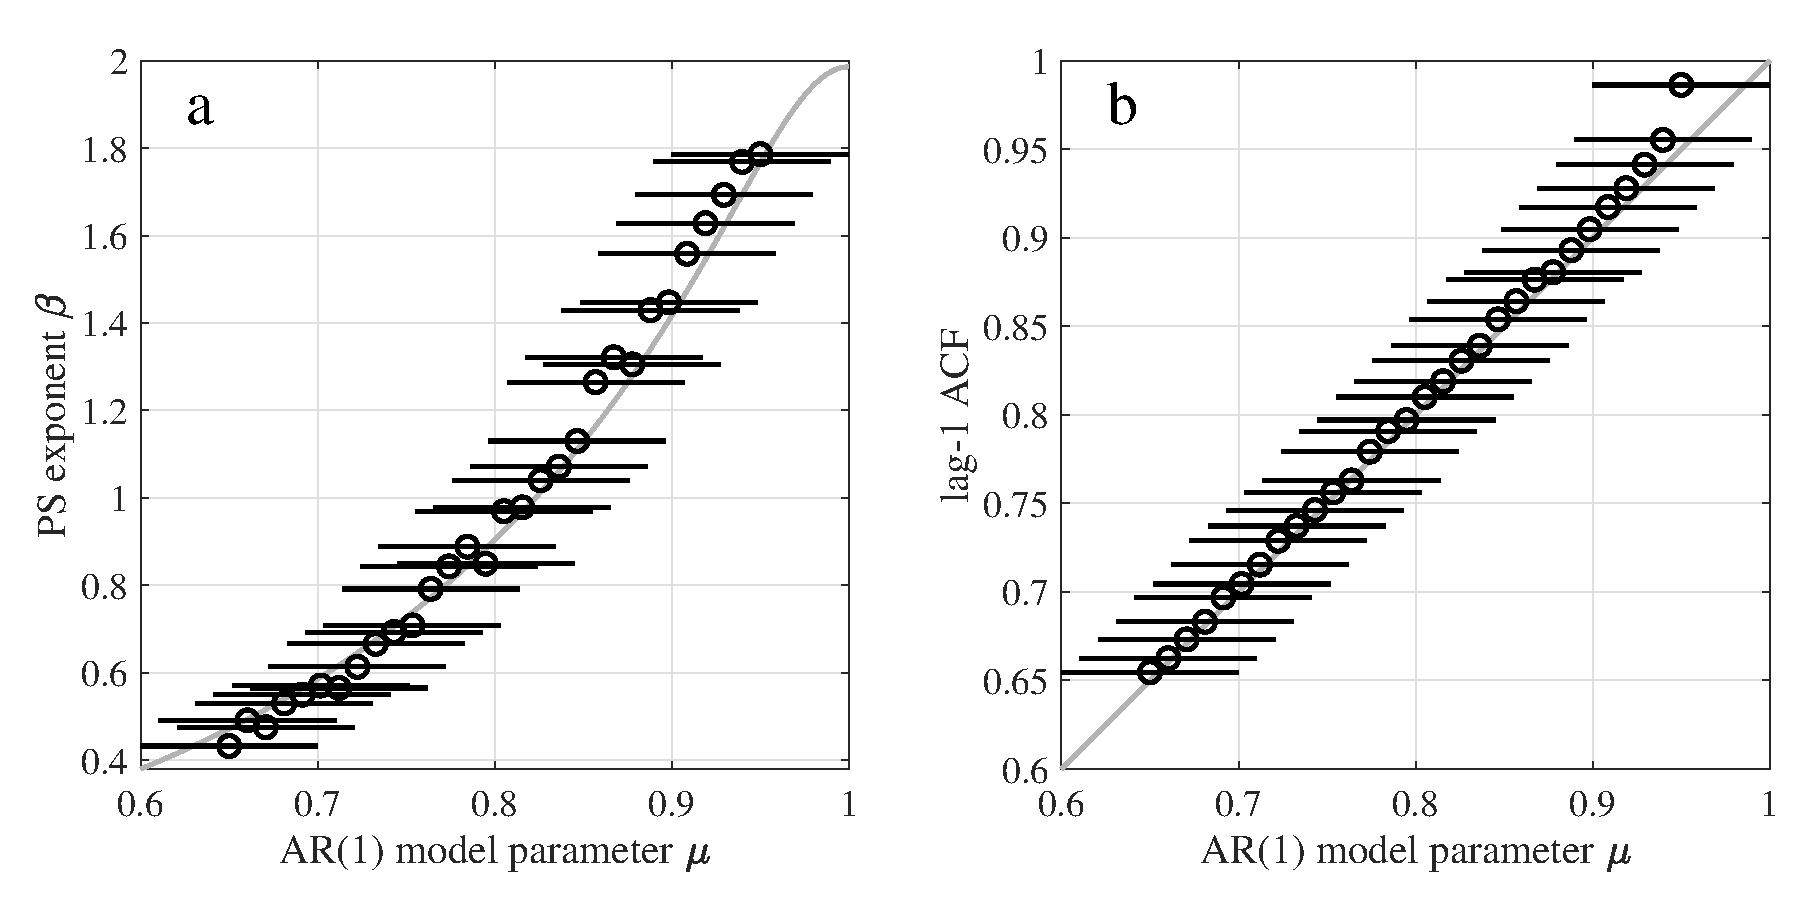
\includegraphics[width=0.9\linewidth]{PS_nonstationary_BigMu}
	\caption{\label{fig:1D:PS_nonstationary_BigMu}
		\Red{[Repeat of the experiment shown in figure~\ref{fig:1D:PS_nonstationary} but with short intervals and considering only values of $\mu$ greater than $0.6$] $30$ time series of length $10^5$ are produced from an AR(1) process with parameter $\mu$ increasing linearly within an interval of values of length $0.1$. only values $\mu\geq0.6$ are considered. The PS exponent (panel {\bf a}) and the lag-1 ACF (panel {\bf b}) are calculated for each time series and the interval of $\mu$ values is plotted against the result in each case. The midpoints of the intervals are marked by circles. A grey line shows, in each case, the true value of $\beta$ or the lag-1 ACF for an AR(1) process with parameter $\mu$.}
	}
\end{figure}

\subsection{Sensitivity of indicators to periodicity}
\label{subsec:1D:Exponents_as_EWS:Periodicity}

{\Red{
In section~\ref{subsec:1D:Exponents_as_EWS:PSsensitivity} we investigated the relationship between the parameter $\mu$ of an AR(1) process and the PS exponent $\beta$ as estimated using the periodogram. We find that for a long enough time series the PS exponent is close to the value predicted by equation~\ref{eqn:1D:PSindicator:reconstruct_mu} which is derived from the equation for the power spectrum of the AR(1) process. We also showed that for a long enough time series the PS exponent is closer to the predicted value than the lag-1 autocorrelation if a parabolic trend is superimposed onto the AR(1) process time series. 

In this section we perform a similar experiment but impose a periodic function (a sine wave) onto the time series. We expect that the PS exponent will not be much affected by this periodicity since adding a sine wave to a time series does not affect the power spectrum beyond adding a single spike at the frequency of the added wave. The PS exponent is determined by taking the linear gradient across a range of frequencies and changing one point will not significantly alter the result. Additionally, if the frequency of the sine wave is outside of the range used in the estimation of the PS exponent, it will not affect the result at all. 
}}

\begin{figure}
	% plotted using the Matlab script 'AR1plusSineWavePlot.m'
	\centering
	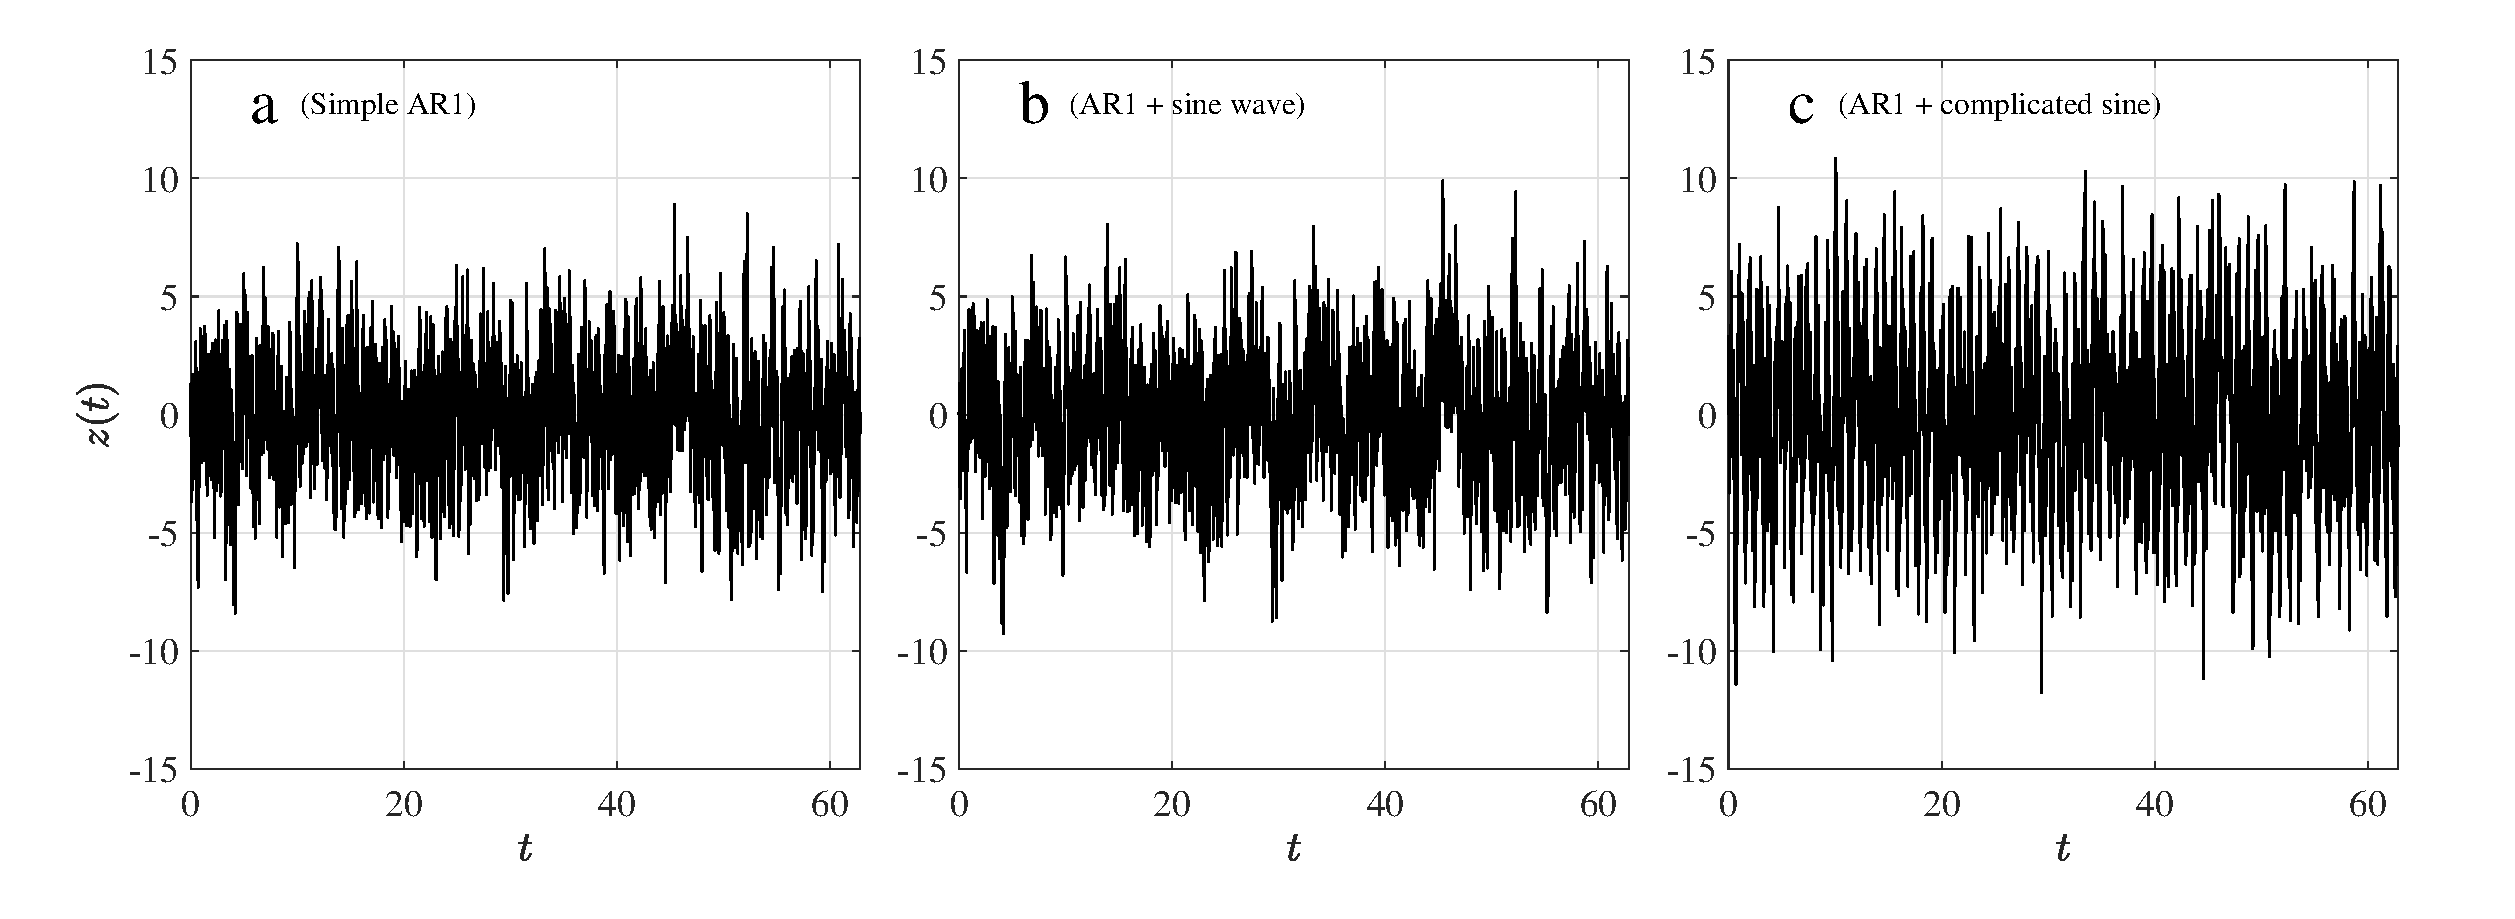
\includegraphics[width=0.9\linewidth]{threeSineWaves}
	\caption{\label{fig:1D:periodicity:threeSineWaves}
		\Red{An AR(1) process of length $10^4$ with parameter $\mu=0.9$ with a periodic function superimposed. Panel {\bf a}: no function. Panel {\bf b}: a simple sine wave $\sin(t)$. Panel {\bf c}: a more complicated function $2\sin(50t)+3\sin(7t)$.}
	}
\end{figure}

{\Red{
In this experiment we take $100$ time series from AR(1) processes
\begin{equation}
	Z_k = \mu Z_{k-1} + \eta_k
\end{equation}
with parameter $\mu$ in the range $[0,1]$. The variance of the Gaussian white noise process $\eta_k$ is $1$. We use time series of length $10^4$ with the artificial time variable $t\in[0, 20\pi]$. From each of these time series $Z(t)$ we create three time series which we use in our analysis:
\begin{enumerate}
	\item The original time series $z(t) = Z(t)$.
	\item The original time series plus a simple sine wave $z(t) = Z(t) + \sin(t)$.
	\item The original time series plus a more complicated function $z(t) = Z(t) + 2\sin(50t)+3\sin(7t)$.
\end{enumerate}
Since the time variable is in the range $[0,20\pi]$, ten periods of the function $\sin(t)$ occur within the time series in each case, whilst $500$ and $70$ periods of the functions $2\sin(50t)$ and $3\sin(7t)$ occur respectively. Each of these is illustrated in figure~\ref{fig:1D:periodicity:threeSineWaves}, which uses $\mu=0.9$ to produce the original AR(1) process. 
}}

\begin{figure}
	% plotted using the Matlab script 'AR1plusSineWavePlot.m'
	\centering
	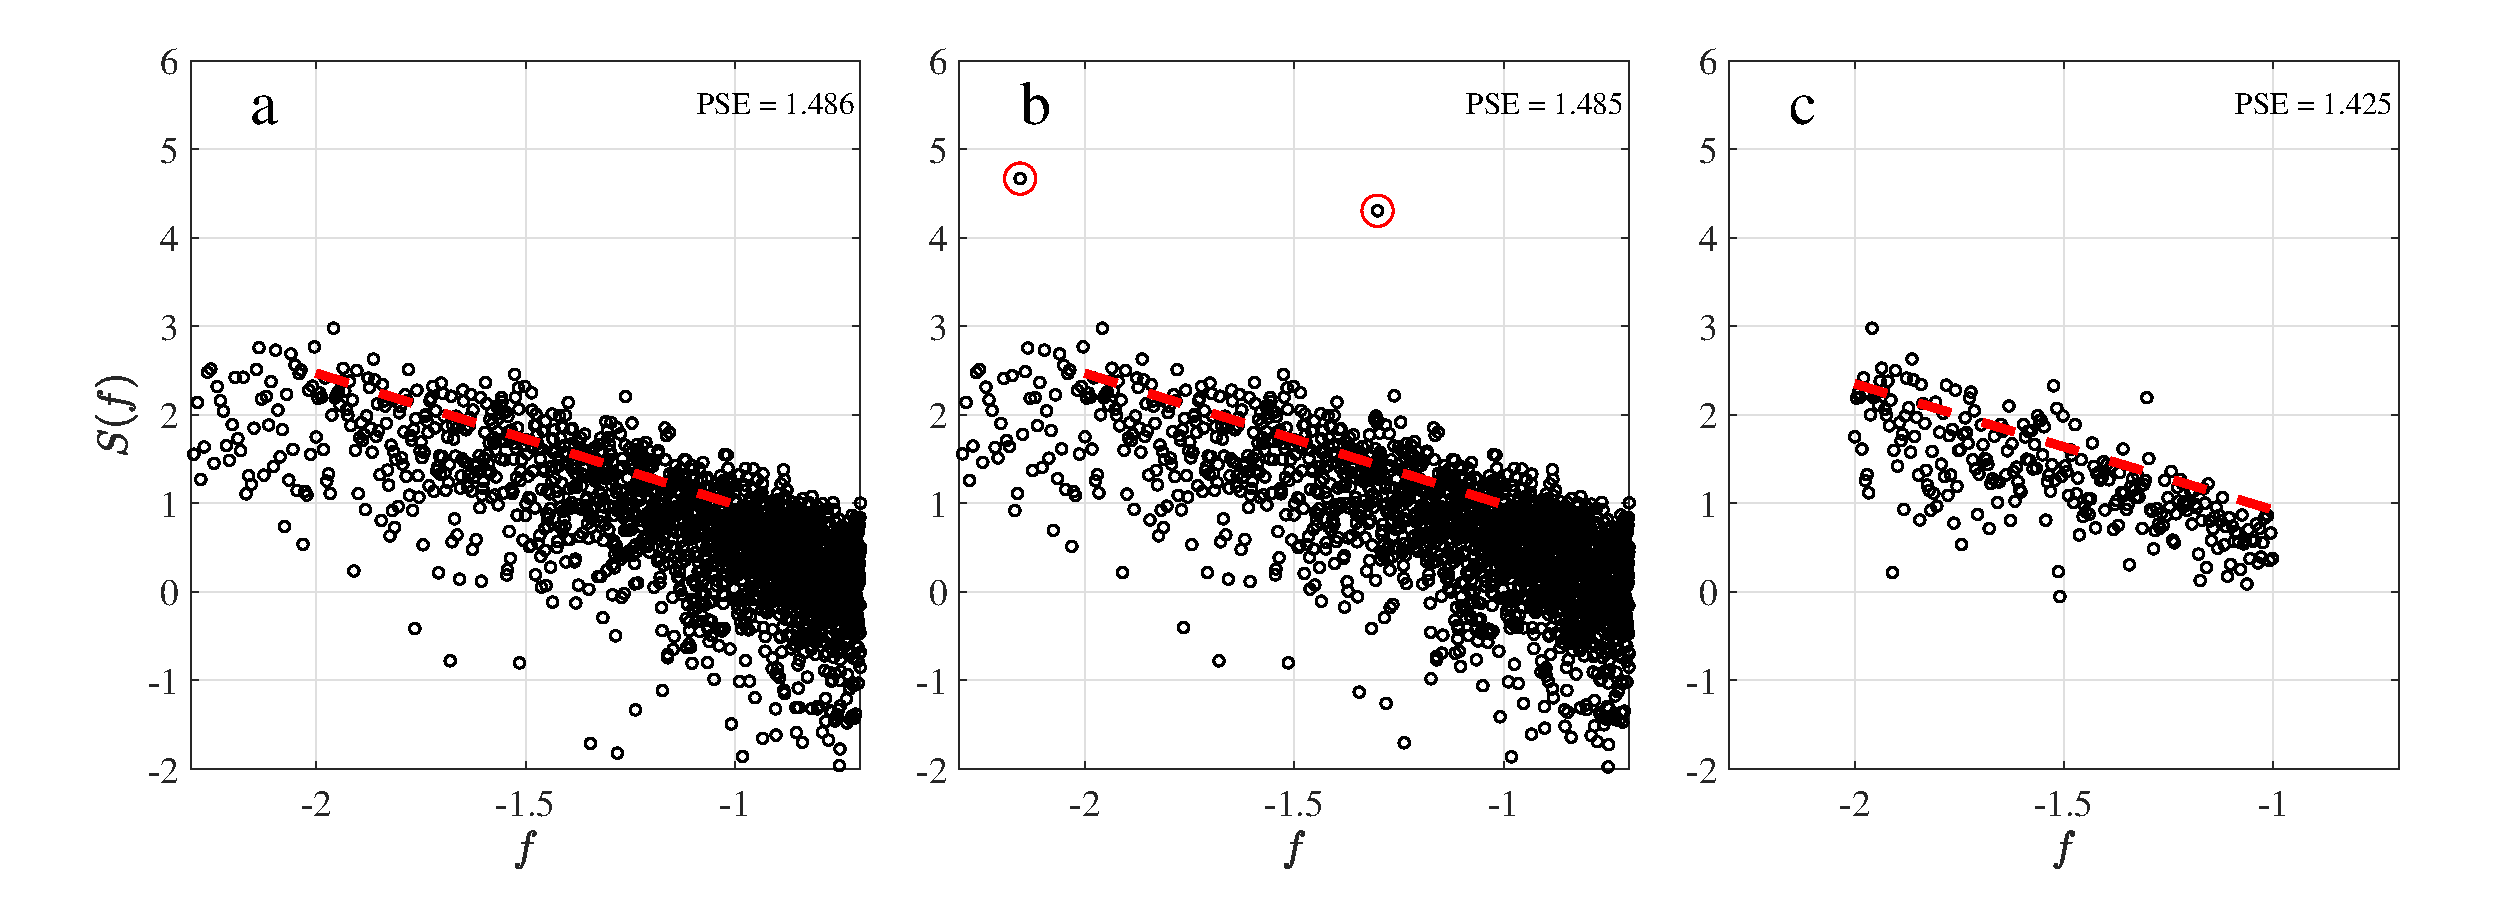
\includegraphics[width=0.9\linewidth]{threePeriodograms}
	\caption{\label{fig:1D:periodicity:threePeriodograms}
		\Red{Panel {\bf a}: periodogram of an AR(1) process.  Panel {\bf b}: periodogram of the same AR(1) process with an added periodic function $g(t) = 2\sin(50t)+3\sin(7t)$. Panel {\bf c}: same as {\bf b} but logarithmic binning has been used. In each case the value of the PS exponent is printed in the top right corner and the line of best fit in the frequency range $\m2\leq\log f\leq\m1$ is plotted in red. The PS exponent for the simple AR(1) process, when using logarithmic binning, is also $1.425$. The power spectrum `spikes' due to the two periodic components are circled in red (panel {\bf b}).  }
	}
\end{figure}

{\Red{
In figure~\ref{fig:1D:periodicity:threePeriodograms} we demonstrate the calculation of the PS exponent for the AR(1) process with $\mu=0.9$. In panels {\bf a} and {\bf b} we compare the periodograms of (respectively) the simple AR(1) process $z(t)=Z(t)$ and the AR(1) with added periodic function $z(t) = Z(t) + 2\sin(50t)+3\sin(7t)$. The power spectral `spikes' due to the two periodic components are circled in red in panel {\bf b}. We note that one spike lies outside of the frequency range used for the estimation of the PS exponent and so will not affect the calculation. The stripped-down periodgram shown in panel {\bf c} of the figure demonstrates the effect of using logarithmic binning to gain a more unbiased estimate of the PS exponent, which is how the exponent is obtained throughout this thesis when using the PS indicator. Once the logarithmic binning is applied the presence of the spikes in the periodogram is even less noticeable, and we find that the value of the PS exponent obtained in this way is the same (to $4$ significant figures) as for the simple AR(1) process without the periodic component. We therefore do not expect that the addition of the periodic series to affect the performance of the PS indicator.

The lag-1 autocorrelation (ACF1), the DFA exponent $\alpha$ and the PS exponent $\beta$ are then calculated for each of these time series and the results are shown in figure~\ref{fig:1D:periodicity:sineWaveAR1}. We note that the ACF1 and DFA are significantly affected by the addition of even a single sine wave with relatively small amplitude (relative to the noise in the AR(1) process, compare figures~\ref{fig:1D:periodicity:threeSineWaves}a and b). As with the introduction of the parabolic trend, the ACF1 is simply scaled up in a consistent way by the introduction of the periodic function, whereas the DFA exponent is affected differently for different values of the parameter $\mu$. The PS exponent, however, is not noticeably affected at all by the introduced periodicity. 
}}

\begin{figure}
	% plotted using the Matlab script 'sineWaveAR1.m'
	\centering
	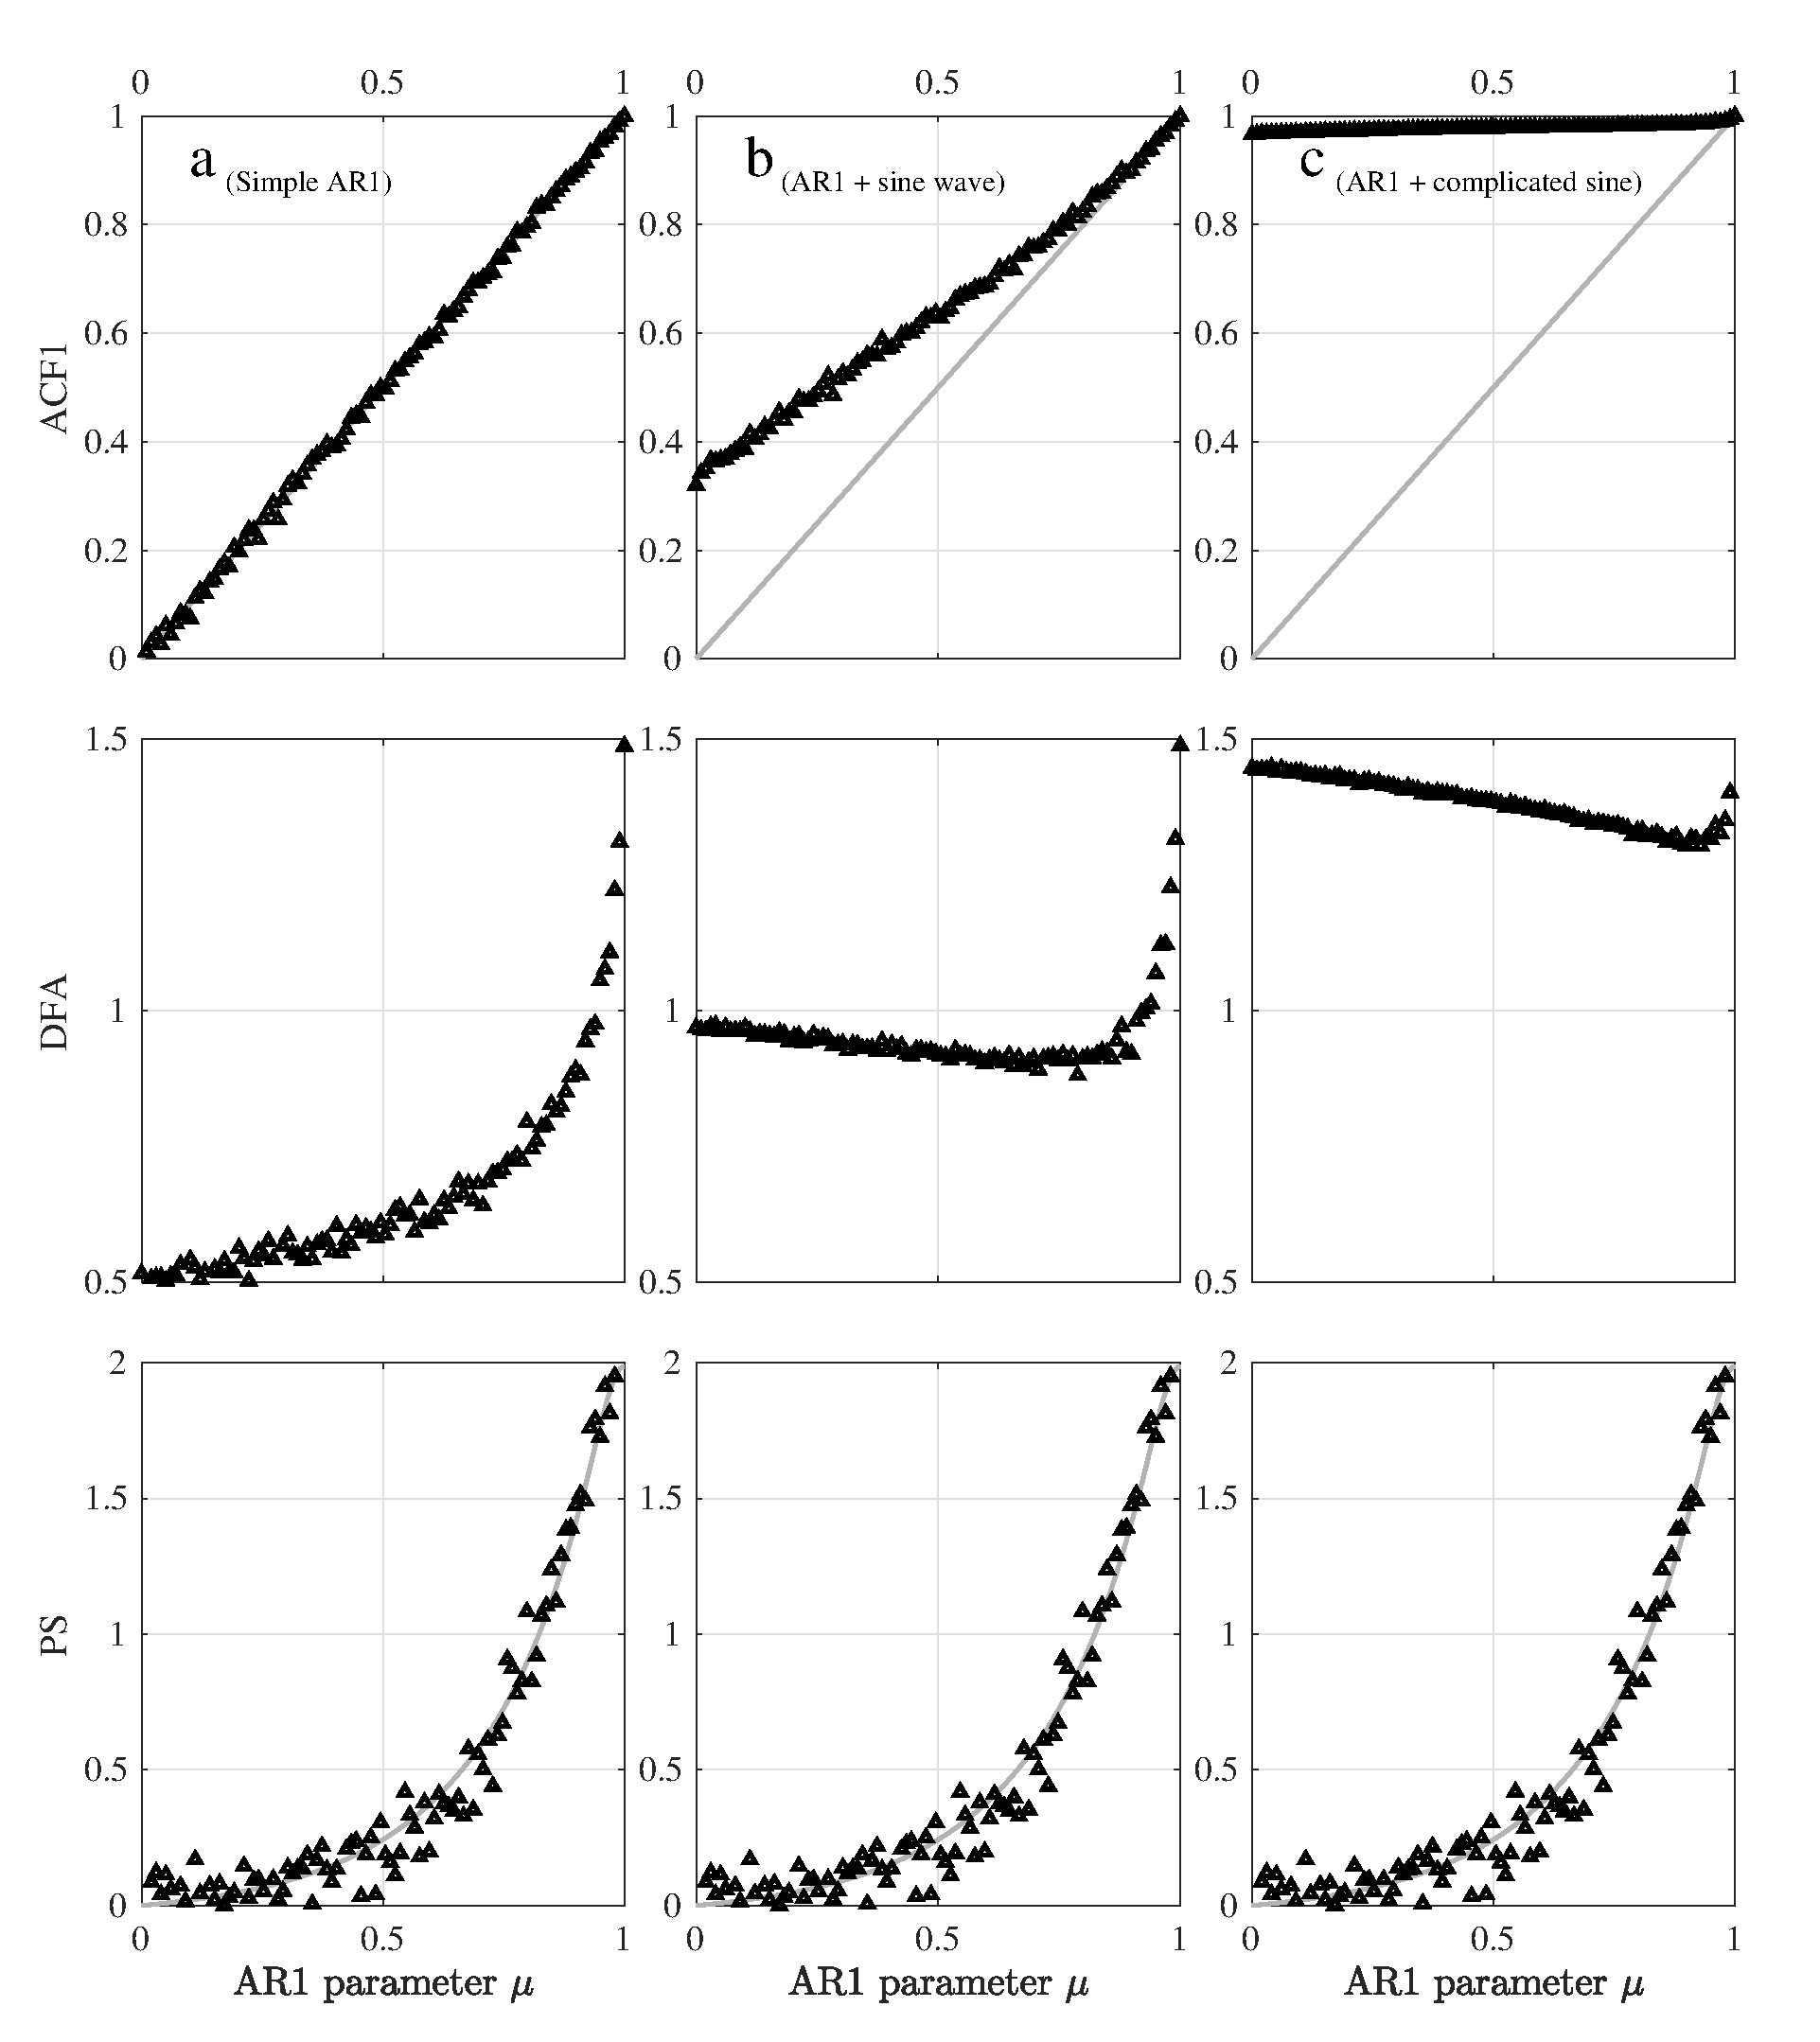
\includegraphics[width=0.9\linewidth]{sineWaveAR1}
	\caption{\label{fig:1D:periodicity:sineWaveAR1}
		\Red{The ACF1 (top row), DFA exponent (middle row) and PS exponent (bottom row) are calculated for $100$ AR(1) time series of length $10^4$ with $\mu\in[0,1]$. The AR(1) time series is super imposed with either no other function (column {\bf a}), a simple sine wave (column {\bf b}), or a more complicated periodic function (column {\bf c}). We note that the PS exponent is practically the same in all three cases. In the case of the ACF1 and PS, the expected value function is plotted in grey.}
	}
\end{figure}

\section{Numerical integration of stochastic ODEs}
\label{sec:1D:numerical_integration}

{\Red 
	
	Throughout this thesis, particularly in this chapter and the next (chapter~\ref{chap:2D}), we obtain a time series by integrating a system of stochastic ODEs (SDEs) and then apply the EWS techniques to this time series, which typically exhibits a tipping point. Such time series, the results of numerical integration of SDEs, have already been presented in chapter~\ref{chap:intro} (see figures~\ref{fig:intro:transitions20_basic} \& \ref{fig:intro:bifurcations20_basic}) without proper explanation of how the integration was performed. 
	
	In initial experiments a simple Euler-Maruyama method, a generalisation of the Euler method to SDEs, was used to integrate one-dimensional systems of the form
		\begin{equation}
		\label{eqn:1D:numerical_integration:standardform}
			\frac{d}{dt}X = f(X,t) + \sigma\eta_t\,,
		\end{equation}
	where $\eta$ is a Gaussian white noise process. Or, using It\^{o} calculus notation,
		\begin{equation}
		\label{eqn:1D:numerical_integration:Ito_form}
			dX = f(X,t)dt + \sigma dW_t\,,
		\end{equation}
	where $W_t$ is a Brownian motion process. For systems of dimension $p>1$, $\eta$ is given as a $p\times 1$ vector and $\sigma$ is a $p\times p$ matrix so that, for example, for the two-dimensional systems of equations
		\begin{equation}
			\begin{array}{rcl}
			\dot{x} &=& y + \sigma_1 \eta^{(x)},\\
			\dot{y} &=& \alpha -  x^2 + \sigma_2\eta^{(y)},
			\end{array}
		\label{eqn:1D:numerical:homoclinicSystem}
		\end{equation}
	where $\eta^{(x)}$ and $\eta^{(y)}$ are two independent Gaussian white noise processes, we have
		\begin{equation}
			f:\begin{pmatrix}
			x\\
			y
			\end{pmatrix}\mapsto \begin{pmatrix}
			y\\
			\alpha - x^2
			\end{pmatrix}\,,
		\end{equation}
	and
		\begin{equation}
			\eta = \begin{pmatrix}
			\eta^{(x)}\\
			\eta^{(x)}
			\end{pmatrix} ~~~\text{and}~~~ \sigma = \begin{pmatrix}
			\sigma_1 & 0\\
			0 & \sigma_2
			\end{pmatrix}\,.
		\end{equation}
	The solution $X(t)$ is approximated by the series $Y_n|_{n=0}^N$ (the Euler–Maruyama approximation), calculated according to
		\begin{equation}
		\label{eqn:1D:numerical_integration:EM_method}
			Y_{n+1} = Y_n + \Delta t f(Y_n,t_n) + \sqrt{\Delta t}\sigma\eta_n\,.
		\end{equation}
	Here the $\eta_n$ are independent identically Gaussian distributed random variables. The $t_n$ form a series with $t_n - t_{n-1} = \Delta t$ and $[t_0, t_N]$ are the lower and upper bounds of integration. The approximation $Y_n$ converges to the true solution $X(t)$ as $\Delta t \rightarrow 0$. 
	
	In several initial experiments in chapter~\ref{chap:2D}, where two-dimensional dynamical systems are presented, the integration of the system of two SDEs was obtained using Matlab's \texttt{ode45} solver \citep{matlab_ode45} which is based on the Dormand-Prince explicit Runge-Kutta (4,5) method \citep{dormand1980family}. This solver is designed for ODEs and does not explicitly handle stochasticity; when including the white noise term $\sigma\eta$ in the solver input, the scaling term $\sqrt{\Delta t}$ was therefore included, as in equation~\ref{eqn:1D:numerical_integration:EM_method}, where $\Delta t$ is specified in the solver input. 
	
	However, Matlab's \texttt{ode45} solver uses an adaptive time step, which may be changed to improve efficiency even if the size of $\Delta t$ is specified by the user. This may then affect the integration of the SDEs since the scaling of the standard deviation of the noise will not be consistent. The Euler-Maruyama method (equation~\ref{eqn:1D:numerical_integration:EM_method}) was therefore used as an alternative, making the method consistent across the thesis, whether dealing with one-dimensional systems given as a single SDE or ODE, or higher dimensional dynamical systems involving systems of two or more SDEs. This is equivalent to the Milstein method for constant $\sigma$ \citep{mackevicius2013introduction}, which is the case in all the two-dimensional systems presented chapter~\ref{chap:2D}. In this chapter (\ref{chap:1D}) and chapter~\ref{chap:cyclones}, however, some models are presented in which the noise scaling factor $\sigma$ is itself a function of time, $\sigma(t)$. The Milstein method, which has superior convergence to the solution \citep{kloeden1999_SDEs}, is therefore used in these cases, where the approximation $Y_n$ is not obtained by equation~\ref{eqn:1D:numerical_integration:EM_method}, but according to 
		\begin{equation}
		\label{eqn:1D:numerical_integration:Milstein}
			Y_{n+1} = Y_n + \Delta t f(Y_n,t_n) + \sqrt{\Delta t}\sigma(t_n)\eta_n + \frac{1}{2}\sigma(t_n)\sigma'(t_n)\Delta t\left((\sigma(t_n) \eta_n)^2-1\right)\,.
		\end{equation}
	where $\sigma'$ is the derivative of $\sigma$ with respect to $X$ and is estimated using 
		\begin{equation}
		\label{eqn:1D:numerical:sigmadash}
			\frac{d}{dx}\sigma = \left(\frac{dt}{dx}\right)^{\m1}\cdot\frac{\partial \sigma}{\partial t} \approx \left(\frac{\Delta t f(Y_n,t_n) + \sqrt{\Delta t}\sigma(t_n)\eta_n}{\Delta t}\right)^{\m1} \cdot \frac{\sigma(t_{n+1})- \sigma(t_n)}{\Delta t}\,,
		\end{equation}
	or 
		\begin{equation}
			\sigma'(t_n) \approx \frac{\sigma(t_{n+1})- \sigma(t_n)}{\Delta t f(Y_n,t_n) + \sqrt{\Delta t}\sigma(t_n)\eta_n}\,,
		\end{equation}
	where we have used the Euler-Maruyama method in the estimation of $dx/dt$. We note that the numerator $\sigma(t_{n+1})- \sigma(t_n)$ ensures that the whole last term in equation~\ref{eqn:1D:numerical_integration:Milstein} is indeed zero where $\sigma$ is constant, thus ensuring that this is equivalent to the Euler-Maruyama method in equation~\ref{eqn:1D:numerical_integration:EM_method}. For systems of dimension $p>1$, equation~\ref{eqn:1D:numerical:sigmadash} becomes problematic since the `numerator' $\dot{\Sigma} := \sigma(t_{n+1})- \sigma(t_n)$ is a $p\times p$ matrix and the `denominator' $\dot{X} := \Delta t f(Y_n,t_n) + \sqrt{\Delta t}\sigma(t_n)\eta_n$ is a $p\times 1$ vector. In this case we perform the element-wise reciprocal operation on $\dot{X}$ and then take the matrix product	
	\begin{equation}
	\sigma'(t_n) = \begin{pmatrix}
	(\dot{x}_1)^{\m1} &  & 0\\
	  & \ddots & \\
	0  &  & (\dot{x}_p)^{\m1}
	\end{pmatrix} \dot{\Sigma}~~~~\text{where}~~~\dot{X} = \begin{pmatrix}
	\dot{x}_1\\
	\vdots\\
	\dot{x}_p\,.
	\end{pmatrix}\,.
	\end{equation}
	Concerning the term $(\sigma(t_n) \eta_n)^2$ in equation~\ref{eqn:1D:numerical_integration:Milstein}, the vector $\sigma(t_n) \eta_n$ is first calculated and the square operation is performed element wise before the vector of ones is subtracted. 
	
	In this chapter many one-dimensional systems are defined by an SDE in the form
		\begin{equation}
		\label{eqn:1D:numerical_integration:potentialform}
			\dot{z}(t) = -\frac{\partial}{\partial z}U(z,t) + \sigma(t)\eta_t\,,
		\end{equation}
	where $U$ is the generalised potential function of $z$ which may also change over time. This formulation is convenient as it allows us to visualise the stable points (troughs or `wells') and unstable points (peaks) of the state space. In these cases the system is not of the form in equation~\ref{eqn:1D:numerical_integration:standardform} since we have the negative derivative of $U$, rather than the function $f$. The function $f$ is either obtained analytically by taking the derivative of $U$ with respect to $z$, in cases where $U$ is a function of $z$ only; or, if this is complicated due to a time dependence in $U$, the function $f$ is estimated at each stage in the Milstein algorithm using 
		\begin{equation}
		\label{eqn:1D:numerical_integration:function_estimate}
			f(Y_n, t_n) = 	-\frac{U(Y_n+\varepsilon, t_n)-U(Y_n-\varepsilon, t_n)}{2\varepsilon}\,,
		\end{equation}
	where the small step $\varepsilon$ is chosen as $\varepsilon=\min(\Delta t, 10^{-5})$ to reduce error over simply using $\varepsilon=\Delta t$ in the case that $\Delta t$ is large, although we typically use small values of $\Delta t$ anyway. 
	
	The Milstein method, given by equation~\ref{eqn:1D:numerical_integration:Milstein} (or the equivalent Euler-Maruyama method where $\sigma$ is constant), is used consistently throughout this thesis for all numerical integration of SDEs, including where system equations are given in the generalised potential form, in which case the function $f$ is estimated using equation \ref{eqn:1D:numerical_integration:function_estimate} if it cannot be obtained analytically.
	
	In cases where Matlab's \texttt{ode45} solver had already been used at the stage of experimentation to integrate two-dimensional systems of SDEs presented in chapter~\ref{chap:2D}, the same systems were integrated again using the Milstein method, in which the scaling of the time step is handled properly, although the method itself is much simpler than the Runge-Kutta (4,5) method with inferior convergence for ODEs \citep{mackevicius2013introduction}. In all cases where both methods were used there was no visible difference between the two, nor any difference in the calculated early warning signals, suggesting that the error due to the adaptive time step problem was, in fact, negligible. Similarly, where the simpler Euler-Maruyama method had been used at the stage of experimentation to integrate one-dimensional SDEs with non-constant $\sigma$, these same systems were integrated again using the Milstein method.
	
	
}



\section{Early Warning Signals in dynamical systems}
\label{sec:1D:indicatorComparison}

{\Red In this section we apply the DFA, PS and ACF1 indicators to several  examples of time series containing tipping points. The first system we study is constructed from segments of generated noise, artificially designed to have a gradually increasing power spectrum scaling exponent, which is used by \cite{livina2012} as a test of the DFA indicator method. We use the same system here to offer a direct comparison between that and the novel PS indicator \citep{prettyman2018}. We then apply the PS indicator and the ACF1 indicator to the three examples presented in chapter~\ref{chap:intro} (see section~\ref{subsec:intro:tippingpoints:defining_a_tipping_point}) which represent the three types of tipping point as outlined by \cite{livina2011}, and also a variety of different bifurcational tipping points occurring in one-dimensional systems. Some of these we go on to study in more detail and also apply the DFA indicator for comparison. In no case do we suppose that there is some critical value of the indicator which gives us special information about a tipping point. Rather, it is the behaviour of the indicator over time which we expect to precede a tipping point. In the cases of the ACF1, DFA and PS indicators used in this chapter, it is an \emph{increasing trend} that we look for, whatever the actual values of the indicators themselves.
		
In this section, and at other points throughout this thesis, a dynamical system is defined analytically as a stochastic ODE and then integrated numerically in Matlab to produce a time series of data. The Milstein method of numerical integration, as defined in the previous section, is used consistently throughout (see section~\ref{sec:1D:numerical_integration}).
}

{\Red{The results of the application to the supercritical pitchfork bifurcation (section~\ref{subsec:1D:indicatorComparison:PitchforkModel}) have previously been presented in \cite{prettyman2018}.}}

\subsection{Choice of model parameters}
\label{subsec:1D:indicatorComparison:choice_of_parameters}
{\Red{
The work presented in this section and, later, in chapter~\ref{chap:2D} makes heavy use of `toy' dynamical system models in our investigation of EWS techniques. Such toy models, particularly those exhibiting a bifurcation, have some critical parameter $\mu$ which is varied within a range of values and the bifurcation or other tipping point occurs in the system when $\mu$ is equal to some critical value $\mu_\text{crit}$. In this case it is necessary to make a choice of the values of this parameter to be used, as well as how fast to vary this parameter if the model involves a changing value. We consider several factors affecting the choice of the parameters:
\begin{enumerate}
	\item That the different values of the parameter demonstrate a significant qualitative change in the system, indicative of a tipping point. It is often the case that if values of the parameter $\mu$ are considered over the interval $[\mu_\text{crit}-\rho, \mu_\text{crit}+\rho]$, where $\rho$ is very small, the real behaviour of the system may not apparently change very much, despite a bifurcation having occurred. This is quite clearly the case for the supercritical pitchfork bifurcation which changes smoothly from the pre-tipping state space to the post-tipping state space, although it may not be so important with fast-diverging `blow up' systems (e.g. subcritical pitchfork bifurcation).
	\item That the rate of change of the parameter is slow relative to the recovery time of the system. This is an essential consideration since the EWS methods studied here are based on detecting critical slowing down which is a measure of decreasing recovery times. 
	\item That the rate of change of the parameter is slow relative to the numerical time step, since no EWS will be visible if a very large change from the pre-tipping state space to the post-tipping state space occurs in a single step. In any case, such a fast-changing parameter would also affect the previous point since the system would not have time to recover. 
\end{enumerate} 
In general, the choice of model parameters is considered with the aim of facilitating a useful comparison between the novel PS indicator and the ACF1 and DFA indicators, often in similar dynamical systems to those in which these existing methods have already been tested (see \cite{livina2007}), which is the purpose of this study. The problem of detecting critical slowing down, and therefore detecting tipping points, in systems with a relatively fast rate of change of critical parameters is a potentially interesting topic for future work, and may be related to the fast-growing field of \emph{rate-induced tipping points} (see \cite{ritchie2016rate}), but it is not within the scope of the work presented here. 

In addition to the choice of tipping-critical model parameters, it is also necessary to select appropriate values for other system parameters. In particular most of the toy models used in this section and in the following chapter are stochastic systems in which the system equations incorporate a white noise process the size of which may greatly affect the behaviour of the system and the performance of the EWS methods. In all cases, the variance of the noise must be large enough that the system is `perturbed' significantly from the stable state, and that there might be some variation within an ensemble of several integrations of the system (in a purely deterministic system there would be no variation between members of the ensemble). Yet, the variance must also be small enough that the noise does not completely mask the deterministic component of the system. In a system defined by the stochastic differential equation
	\begin{equation}
		\dot{z} = f(z,t) +\sigma\eta\,,
	\end{equation}
where $\eta$ is a Gaussian white noise process, if $\sigma$ is very large compared to the value of $f(z,t)$ for $z,t$ in the range of integration, the integrated time series $z(t)$ will be essentially a random walk, and incorporate none of the deterministic dynamics of the function $f$. In cases where we expect to see noise-induced tipping, and we aim to assess the usefulness of the early warning indicators in that context, the variance of the noise is of course chosen that noise-induced tipping may indeed be observed. Where such noise-induced tipping is brought about by a change the stochastic component of the system, where the variance of the noise term is a parameter with some critical value at which tipping occurs, the rate of change of this parameter is chosen, as with deterministic parameters, such that the tipping may be observed in the integrated time series and that the rate of change is not on time scales faster than the deterministic evolution of the system.  
}}
	



\subsection{Early warning signals in an artificial stochastic signal}
\label{sec:1D:ArtificialModel} 

\begin{figure}
	\centering
	
\includegraphics[width = 0.9\textwidth]{fig2_v5}
	\caption{Artificial data with ACF1, DFA and PS indicators. (a) A time series is constructed by concatenating 50 sub-series of length 200 where the scaling exponent $\beta$ within each sub-series is constant and increases over the whole series from 0 (white noise) to 2. (b,c,d) The ACF1, DFA and PS indicator methods are applied with window size 100. As the PS-indicator increases from 0 to 2, the ACF indicator increases from 0 to 1, and the DFA indicator $\alpha$ increases from 0.5 to 1.5. Lines are added to show the linear trends; note that the ACF indicator does not increase linearly as it approaches 1. \label{fig:1D:ArtificialSignal}}
\end{figure}

 \citet{livina2012} compare the performance of the ACF1 and DFA indicators when applied to an artificially constructed time series with increasing PS scaling exponent. The series is created by concatenating many shorter sub-series with specific, incrementally increasing power spectrum scaling exponents $\beta$ from white noise ($\beta=0$) in the first sub-series to red noise ($\beta=2$) in the final series.  
 
 Here, we recreate the experiment in order to compare the ACF1, DFA and PS indicators. We create 50 sub-series each of length 200 points with incrementally increasing PS exponents. To achieve this, for each sub-series we take a white noise signal $X(t)$, apply a fast Fourier transform and then multiply the power spectrum $\hat{X}(f)$ by a factor of $\sqrt{f^{-\beta}}$ where $\beta$ is the desired PS exponent (see also equation \ref{eqn:1D:creatingColouredNoise}). The resulting power spectrum is then transformed back to the time domain using an inverse fast Fourier transform \citep{makse1996}. The values of $\beta$ increase linearly in the range $[0, 2]$, changing from white noise to red noise. The 50 series are then joined to create a series of length $10^4$. We note that this is an example of a time series which experiences a rise in autocorrelation simultaneously with a decrease in variance. 
 
 
 
The ACF1, DFA and PS indicators are applied to the constructed series. Since the series is specifically constructed to have an increasing PS exponent, we expect to see an increasing trend in the PS indicator. We also expect the same behaviour in the DFA indicator because of the relationship between the two exponents (see figure \ref{fig:1D:ExponentRelationships}). We also know that lag-1 ACF increases with increasing PS exponent in long-range correlated noise (figure \ref{fig:1D:ACFrelationships}) and so expect that the ACF1 indicator will also show an increasing trend when applied to our series.

Figure \ref{fig:1D:ArtificialSignal} shows the signal (panel {\bf a}) and the results of applying the three indicators (panels {\bf b}, {\bf c}, {\bf d}) along with the linear best fit. As in our previous experiment which calculated the lag-1 ACF for noise series with different values of $\beta$ (figure \ref{fig:1D:ACFrelationships}), the lag-1 ACF increases linearly with increasing $\beta$ only up to a point, approximately $\beta = 1$, after which the rate of increase slows. The DFA and PS increase linearly, as expected, with increasing $\beta$ and the relationship between the two indicators obeys the same linear law connecting to DFA and PS exponents (equations \ref{eqn:1D:alphabetaExponentRelationships}). The variance in both indicator series is also similar, and so we have evidence for the assertion that it is not necessary to use the PS exponent when the DFA exponent is available \citep{heneghan2000}, but concerning the sliding-window indicator methods, rather than a simple calculation of the exponents.

\begin{landscape}
	\begin{figure}
		\centering
		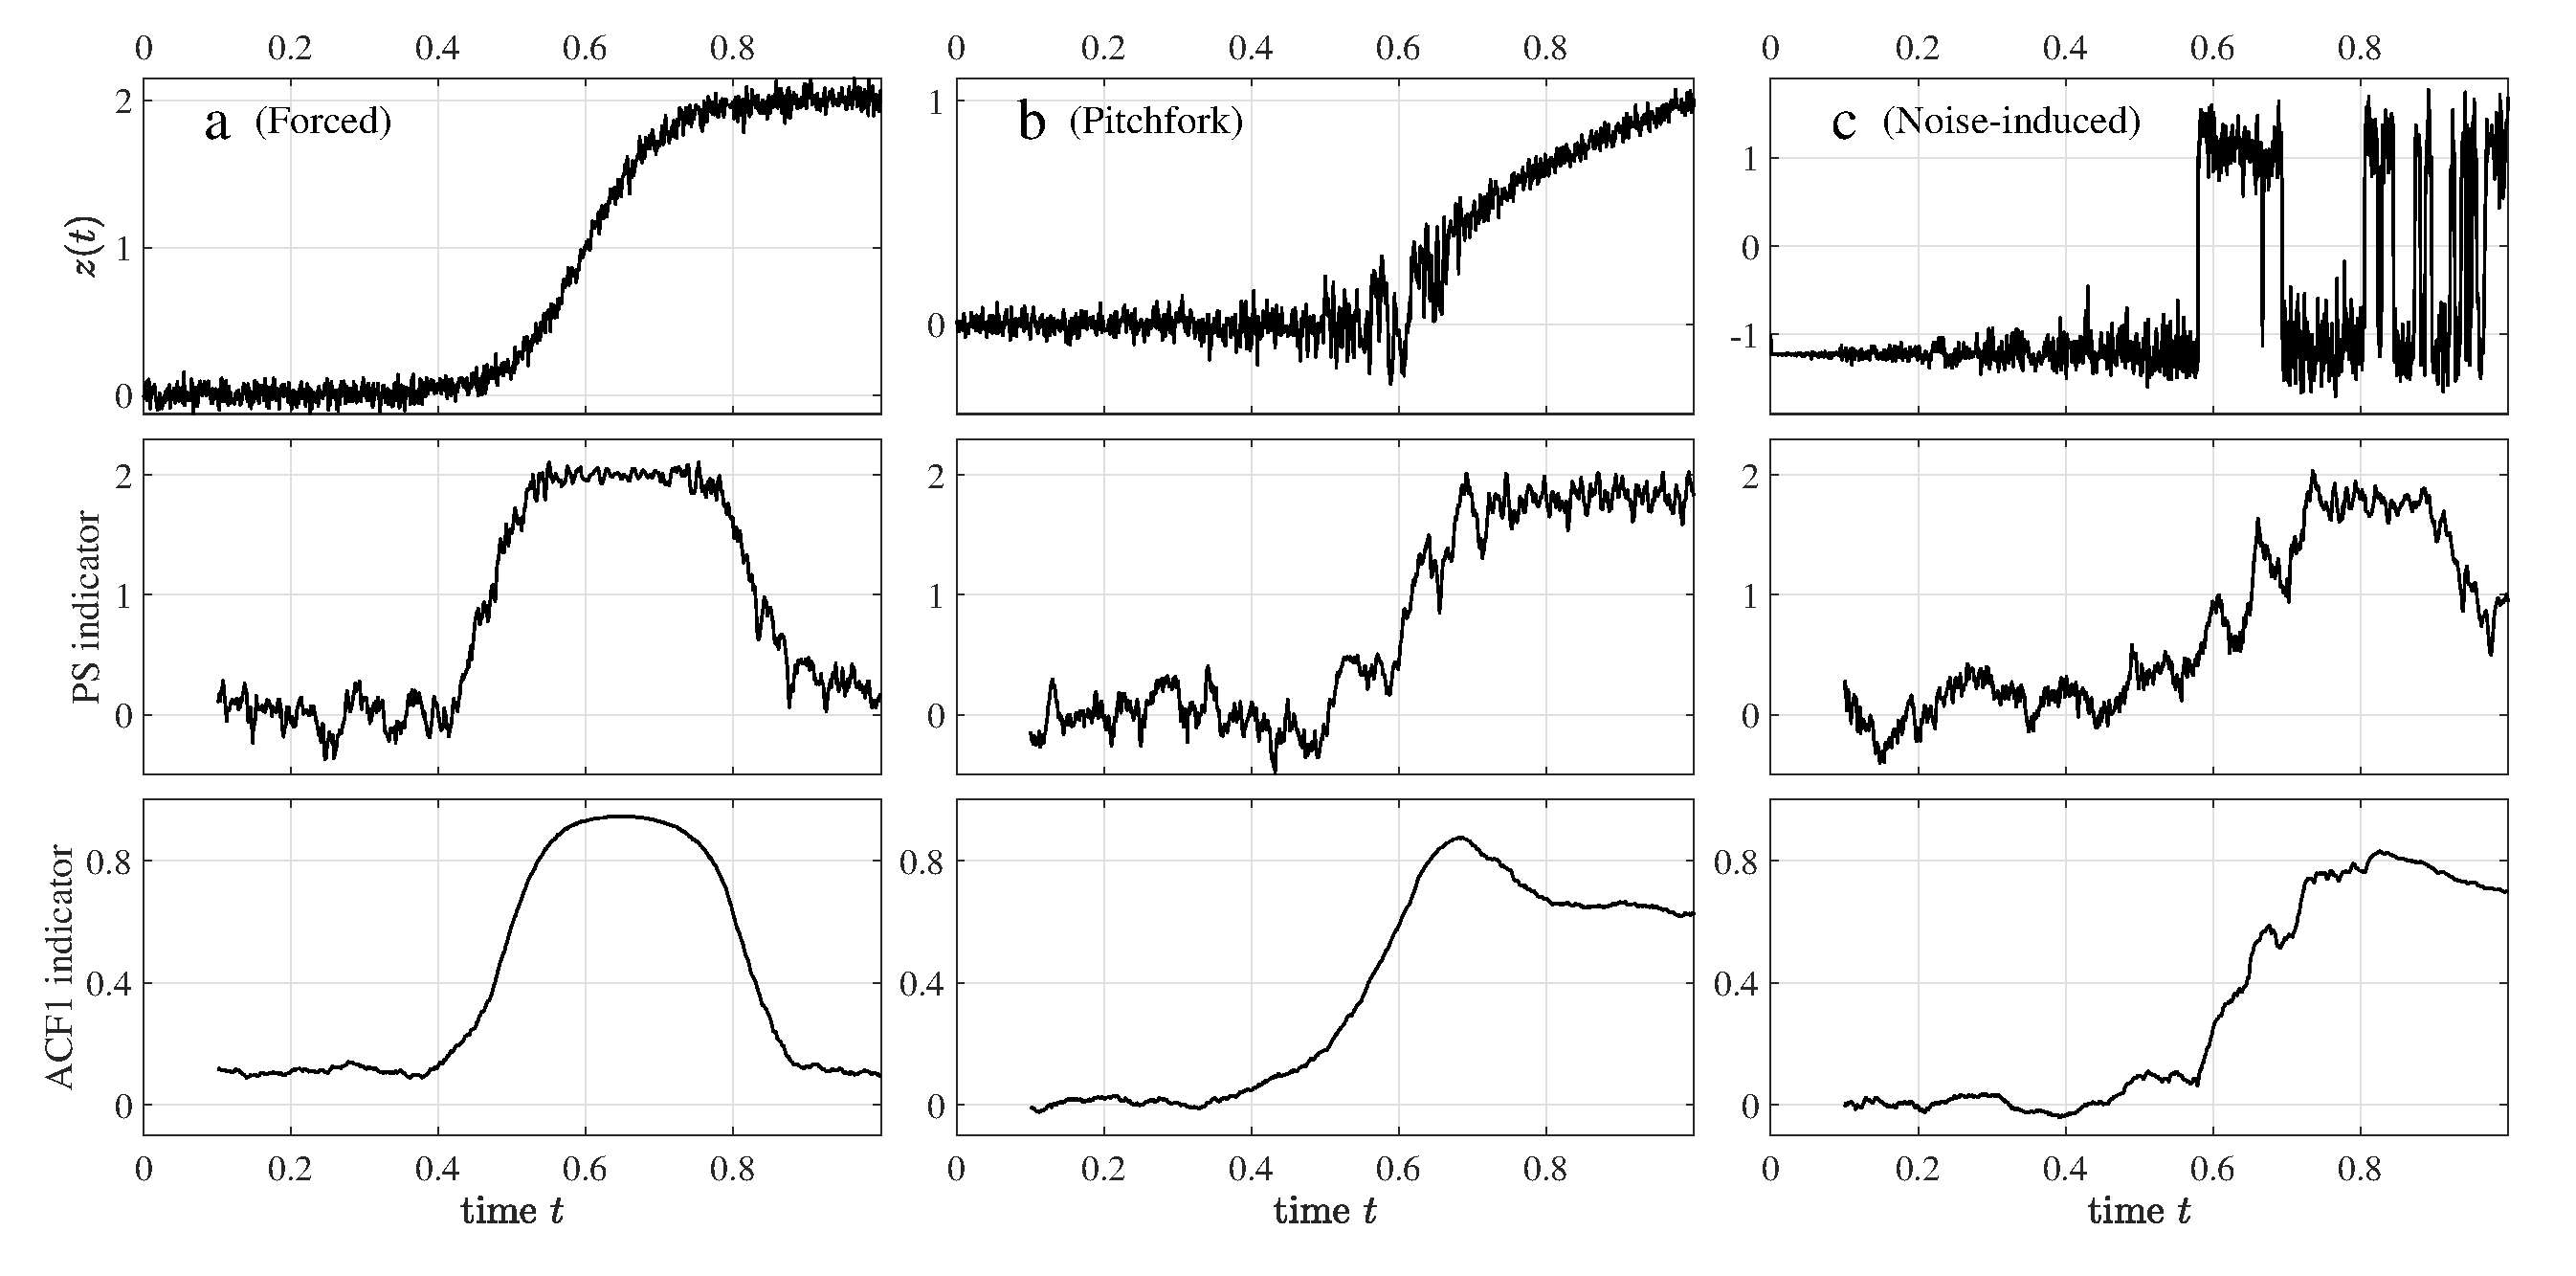
\includegraphics[width=\linewidth,keepaspectratio]{transitions30}
		\caption{\Red{Three systems given by equations~\ref{eqn:1D:DifferentTypesOfTipping:forced} (forced transition), \ref{eqn:1D:DifferentTypesOfTipping:genuine} (pitchfork bifurcation), and \ref{eqn:1D:DifferentTypesOfTipping:noise-induced} (noise-induced tipping point) are integrated between $t=0$ and $t=1$. Each exhibits a tipping point at around $t=0.6$: a forced transition, a pitchfork bifurcation, and a noise-induced transition (panels {\bf a}, {\bf b}, {\bf c} respectively). The PS and ACF1 indicators are calculated using a sliding window of 100 points and plotted beneath the time series for each system. We note the similarity in shape between the two indicator signals, although the PS indicator is more noisy. }
		}
		\label{fig:1D:threesystemswithPSandACF}
	\end{figure}
\end{landscape}

\subsection{Early warning signals for three distinct tipping points}
 \label{subsec:1D:indicatorComparison:TypesOfTipping}

{\Red
 In section~\ref{sec:intro:classification_of_TPs}, chapter~\ref{chap:intro}, we presented three examples of dynamical systems each exhibiting one of the three types of tipping point suggested by \cite{livina2011}: A forced transition, a genuine bifurcation, and a noise-induced transition. 
 
 We give the equations for each of these three examples again here. In each case the system equation is in the `generalised potential' form of equation~\ref{eqn:1D:numerical_integration:potentialform} and integrated numerically using the Milstein method (see section~\ref{sec:1D:numerical_integration}) with time step $\Delta t = 10^{\m 5}$ and a sampling rate of $10^3$ per unit time. Thus each integration generates a time series of $1000$ points since the time range in each case is $t\in [0,1]$.

\subsubsection{Type 1: Forced transition}
As an example of a `forced transition' we use the system described by the equation 
\begin{equation}
\label{eqn:1D:DifferentTypesOfTipping:forced}
\dot{z}(t) = -\frac{\partial }{\partial z}\left(z-\tanh(10t-6)-1\right)^2 + \frac{1}{10}\eta \, ,
\end{equation}
where $\eta$ is a Gaussian white noise process. This system has a quadratic-shape generalised potential which shifts in position over time. For small $t$, that is $t<0.5$, the stable equilibrium, the base of the `well', is at the position $z\approx 0$. This shifts to the position $z\approx 2$ when $t>0.7$. Thus, a sudden shift occurs around $t=0.6$, as we can see in figure~\ref{fig:1D:threesystemswithPSandACF}a. 

We note that both the PS and ACF1 indicators begin to rise about the same time that the shift in the stable point becomes visually obvious, and have reached their maximum values before the system is halfway through the transition. 

\subsubsection{Type 2: Genuine bifurcation}
As an example of a genuine bifurcation we present the familiar pitchfork bifurcation, already used as an example in this chapter, given by the equation:
	\begin{equation}
	\label{eqn:1D:DifferentTypesOfTipping:genuine}
		\dot{z}(t) = -\frac{\partial }{\partial z}\left(z^4+(3-5t)z^2\right) + \frac{1}{10}\eta\,,
	\end{equation}
where $\eta$ is a Gaussian white noise process. In this case the bifurcation occurs at $t=0.6$. We see in figure~\ref{fig:1D:threesystemswithPSandACF}b the apparent increase in ``white'' noise just before $t=0.6$ as the base of the `well' flattens out and allows for longer and longer return times to the equilibrium point $z=0$.

Again we note that the PS and ACF1 indicators show similar behaviour, although the PS indicator is more noisy. In both cases the increasing trend in the indicator begins before the bifurcation occurs at $t=0.6$.


\subsubsection{Type 3: Noise-induced transition}
As an example of a noise-induced transition we take a `double-well' generalised potential with added noise and allow the standard deviation of the noise to increase with time. At some \emph{critical point} the noise is large enough that the system is able to escape from the `well' and switch to the other stable state. The time series in figure~\ref{fig:1D:threesystemswithPSandACF}c is described by the equation:
\begin{equation}
\label{eqn:1D:DifferentTypesOfTipping:noise-induced}
\dot{z}(t) = -\frac{\partial }{\partial z}\left(z^4-3z^2\right) + \frac{3t}{2} \eta\,,
\end{equation}
where $\eta$ is a Gaussian white noise process and the coefficient $\sigma(t) = 3t/2$ modifies the standard deviation of the noise as a function of $t$. At around $t=0.6$ the noise standard deviation is close to $1$ which is about large enough that state-switching becomes likely though not frequent. As $t$ increases further, the frequency of the state-switch increases. 

Once again we note the correlation between the PS and ACF1 indicators. In this example the increasing trend in the indicators does not begin until the noise is already large enough that the system is able to tip into the other stable state. This is due simply to the shape of the generalised potential function in this particular case. For this type of system where a Gaussian white noise process is integrated, an increase in the size of the noise will always cause an increase in the PS exponent, whether it leads to a tipping point or not. This type of tipping is not characterised by the critical slowing down phenomenon, unlike the pitchfork bifurcation of the previous example. We don't therefore expect that the PS indicator will necessarily provide an EWS, although it will, of course, provide information about the nature of the noise in the series. 
 

}


\begin{landscape}
	\begin{figure}
		\centering
		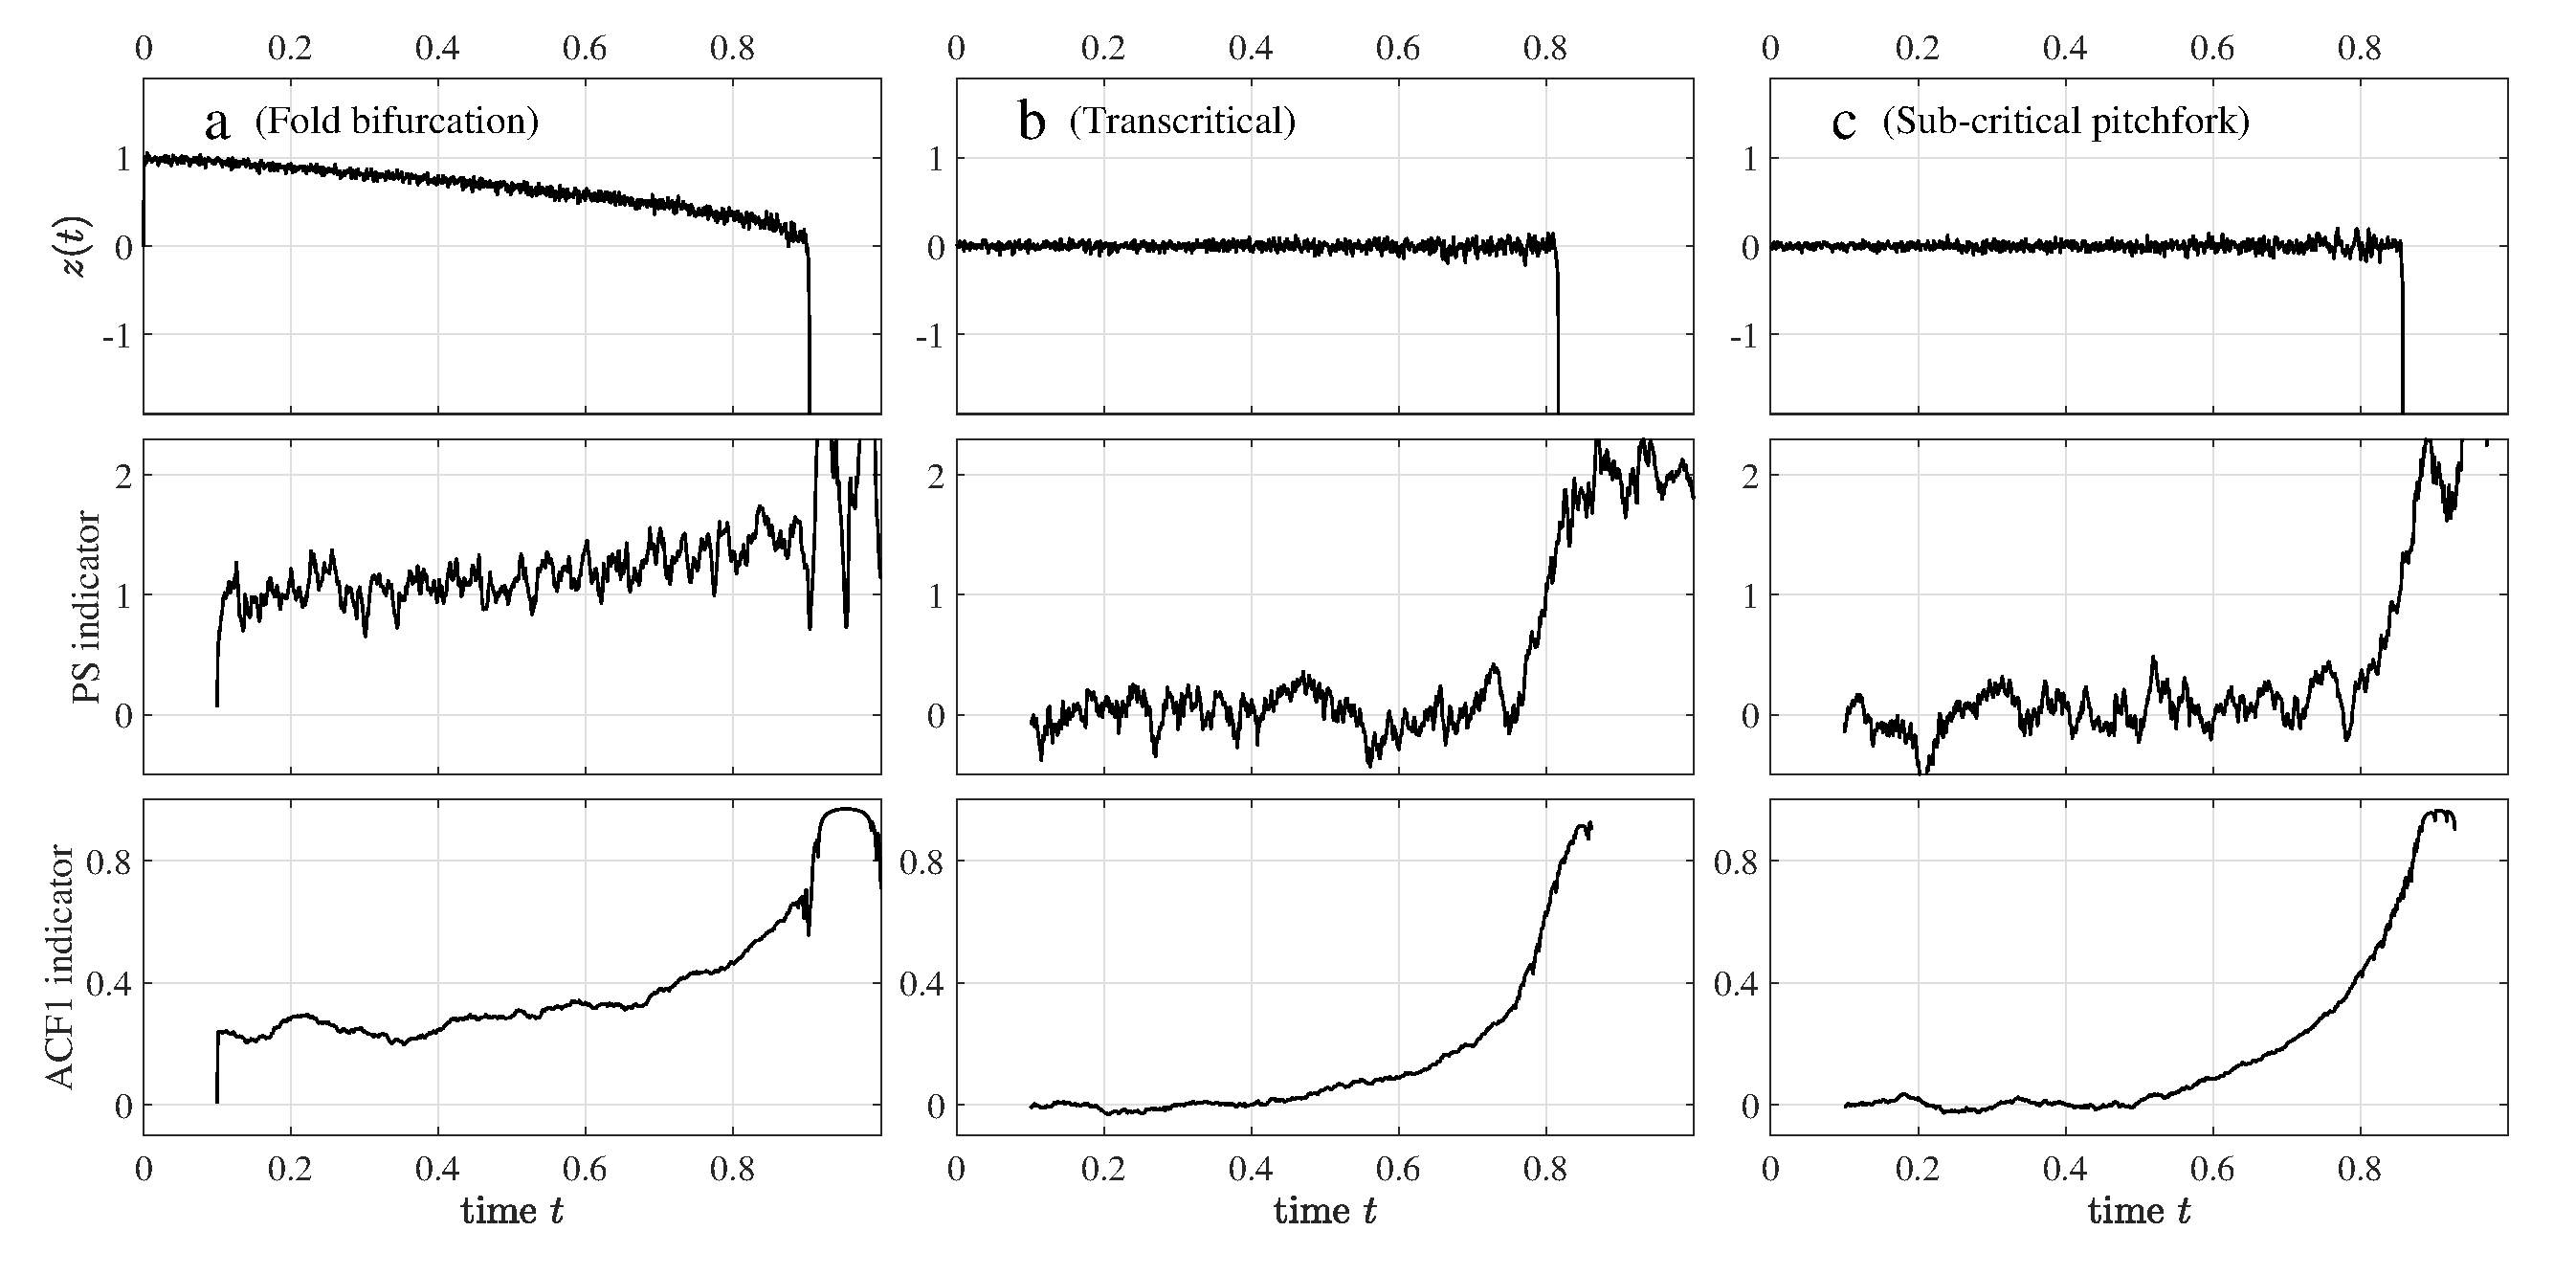
\includegraphics[width=\linewidth,keepaspectratio]{bifurcations30}
		\caption{\Red{Three systems given by equations~\ref{eqn:1D:TypesOfBifurcation:fold} (fold bifurcation), \ref{eqn:1D:TypesOfBifurcation:transcritical} (transcritical bifurcation), and \ref{eqn:1D:TypesOfBifurcation:sub-critical} (sub-critical pitchfork bifurcation) are integrated between $t=0$ and $t=1$. Each exhibits a bifurcation at around $t=0.9$: a fold, transcritical, and sub-critical pitchfork bifurcation (panels {\bf a}, {\bf b}, {\bf c} respectively). The PS and ACF1 indicators are calculated using a sliding window of 100 points and plotted beneath the time series for each system. We note the similarity in shape between the two indicator signals, although the PS indicator is more noisy. }
		}
		\label{fig:1D:TypesOfBifurcation:threesystemswithPSandACF}
	\end{figure}
\end{landscape}

\subsection{Early warning signals for three bifurcational tipping points}
\label{subsec:1D:indicatorComparison:TypesOfBifurcation}

{\Red
	In section~\ref{sec:intro:bifurcation_varieties}, chapter~\ref{chap:intro}, we presented three examples of dynamical systems each exhibiting a different bifurcation implying a tipping point: a fold bifurcation, a transcritical bifurcation and a sub-critical pitchfork bifurcation.
	
	We give the equations for each of these three examples again here. In each case the system equation is in the `generalised potential' form of equation~\ref{eqn:1D:numerical_integration:potentialform} and integrated numerically using the Milstein method (see section~\ref{sec:1D:numerical_integration}, page~\pageref{sec:1D:numerical_integration}) with time step $\Delta t = 10^{\m 5}$ and a sampling rate of $10^3$ per unit time. Thus each integration generates a time series of $1000$ points since the time range in each case is $t\in [0,1]$. The results of all three experiments are shown in figure~\ref{fig:1D:TypesOfBifurcation:threesystemswithPSandACF}
	
	\subsubsection{Type 1: Fold bifurcation}
	The fold bifurcation is a very simple example of a tipping point and has been used to model a wide variety of phenomena, notably in the field of \emph{catastrophe theory} \citep{zeeman1977catastrophe, arnold1999bifurcation}. We consider a dynamical system given by the equation
	\begin{equation}
	\label{eqn:1D:TypesOfBifurcation:fold}
		\dot{z}(t) = -\frac{\partial }{\partial z}\left(z^3+\frac{(10t-9)}{3}z\right),
	\end{equation}
	where $\mu = (10t-9)/3$ is the model parameter. The bifurcation occurs at $\mu=0$, $t=0.9$ when the stable equilibrium at $z=\m\sqrt{\mu/3}$ meets the unstable equilibrium at $z=+\sqrt{\mu/3}$. After this point the system `blows up' since $z$ diverges to infinity. In figure~\ref{fig:1D:TypesOfBifurcation:threesystemswithPSandACF}a we see that both the PS and ACF1 indicators show an increasing trend before the bifurcation occurs, but in the PS indicator this is barely noticeable. 


	
	\subsubsection{Type 2: Transcritical bifurcation}
	The transcritical bifurcation is so named because the equilibria \emph{cross} the critical point: they are not created nor eliminated. Instead, the stable equilibrium becomes unstable and \emph{vice versa}. The normal form of the transcritical bifurcation is
	\begin{equation}
	\dot{z}(t) = -\frac{\partial }{\partial z}\left(z^3-\mu z^2\right),
	\label{eqn:1D:TypesOfBifurcation:transcritical}
	\end{equation}
	which has the same (cubic) shaped generalised potential function as the fold bifurcation normal form. When $\mu=0$, this example has a stable equilibrium at $z = 2\mu/3$ and an unstable equilibrium at $z=0$. At the critical point $\mu=0$ the equilibria are lost momentarily but reappear for $\mu>0$ when the $z=0$ state has become unstable and the (positive) $z = 2\mu/3$ state is now stable. Because of the continuity of the equilibrium at $z=0$, this type of equation is used frequently in biology when zero is often a stable state \citep{nicolis2007,strogatz2014}, for example in population dynamics (of bacteria, humans, etc.) a population of zero is a stable population. Indeed, the above equation has the same form as the logistic equation \citep{brown2018introduction}. In figure~\ref{fig:1D:TypesOfBifurcation:threesystemswithPSandACF}b we see, again, that the ACF1 and PS indicators have a similar shape but that the PS indicator is more noisy and the increasing trend is not visible until closer to the tipping point.
	
	\subsubsection{Type 3: Sub-critical pitchfork bifurcation}
	We have seen already the super-critical pitchfork bifurcation, equation~\ref{eqn:1D:DifferentTypesOfTipping:genuine}, used as an example of a genuine bifurcation in comparison to other types of tipping points (see figure~\ref{fig:1D:threesystemswithPSandACF}b). The contrasting \emph{sub}-critical pitchfork bifurcation has the normal form
	\begin{equation}
	\label{eqn:1D:TypesOfBifurcation:sub-critical}
	\dot{z}(t)  = -\frac{\partial}{\partial z}\left(\m z^4 - \mu z^2\right),
	\end{equation}
	and for $\mu<0$ has a single stable equilibrium at $z=0$ and two unstable equilibria at $z=\pm\sqrt{\m\mu/2}$. At the critical point $z=0$ the two unstable equilibria meet the stable point and develop into a single unstable equilibrium for $\mu>0$. Thus, a system following the stable trajectory will abruptly become unstable at the critical point and quickly diverge to $\pm\infty$ given any small perturbation. Of course, in cases with higher order terms in the equation, the system may in fact converge again to a separate stable point away from $z=0$. As with the fold bifurcation, we see in figure~\ref{fig:1D:TypesOfBifurcation:threesystemswithPSandACF}c that the ACF1 and PS indicators have a similar shape but that the PS indicator is more noisy and the increasing trend is not visible until closer to the tipping point.

	
}

\subsection{The supercritical pitchfork bifurcation model}
 \label{subsec:1D:indicatorComparison:PitchforkModel}

{\Red{
		\subsubsection{Indicators applied}
		We have already looked at a dynamical system experiencing a supercritical pitchfork bifurcation (see figure~\ref{fig:1D:threesystemswithPSandACF}b, page~\pageref{fig:1D:threesystemswithPSandACF}) in comparison to other types of tipping points, and we have seen how well the PS indicator provides an EWS for this system in comparison with the ACF1 indicator. In this section we look more closely at the result in figure~\ref{fig:1D:threesystemswithPSandACF}b and also calculate the EWS given by the DFA indicator. In addition, we address the problem of \emph{predicting}, rather than merely detecting, a tipping point, using this dynamical system as our example.
The dynamical system is, as in section~\ref{subsec:1D:indicatorComparison:TypesOfTipping}, given by the equation
	\begin{equation}
	\label{eqn:1D:EWS:Pitchfork}
		\dot{z}(t) = -\frac{\partial }{\partial z}\left(z^4-(5t-3)z^2\right) + \frac{1}{10}\eta\,,
	\end{equation}
where $\mu=(5t-3)$ is our model parameter and the bifurcation occurs at $\mu=0\Rightarrow t=0.6$. For $\mu<0$ the system has a single stable equilibrium at $z=0$. This becomes unstable for $\mu>0$ and two new stable points develop at $z = \pm\sqrt{\mu}$. }}

\begin{figure}
	\centering
	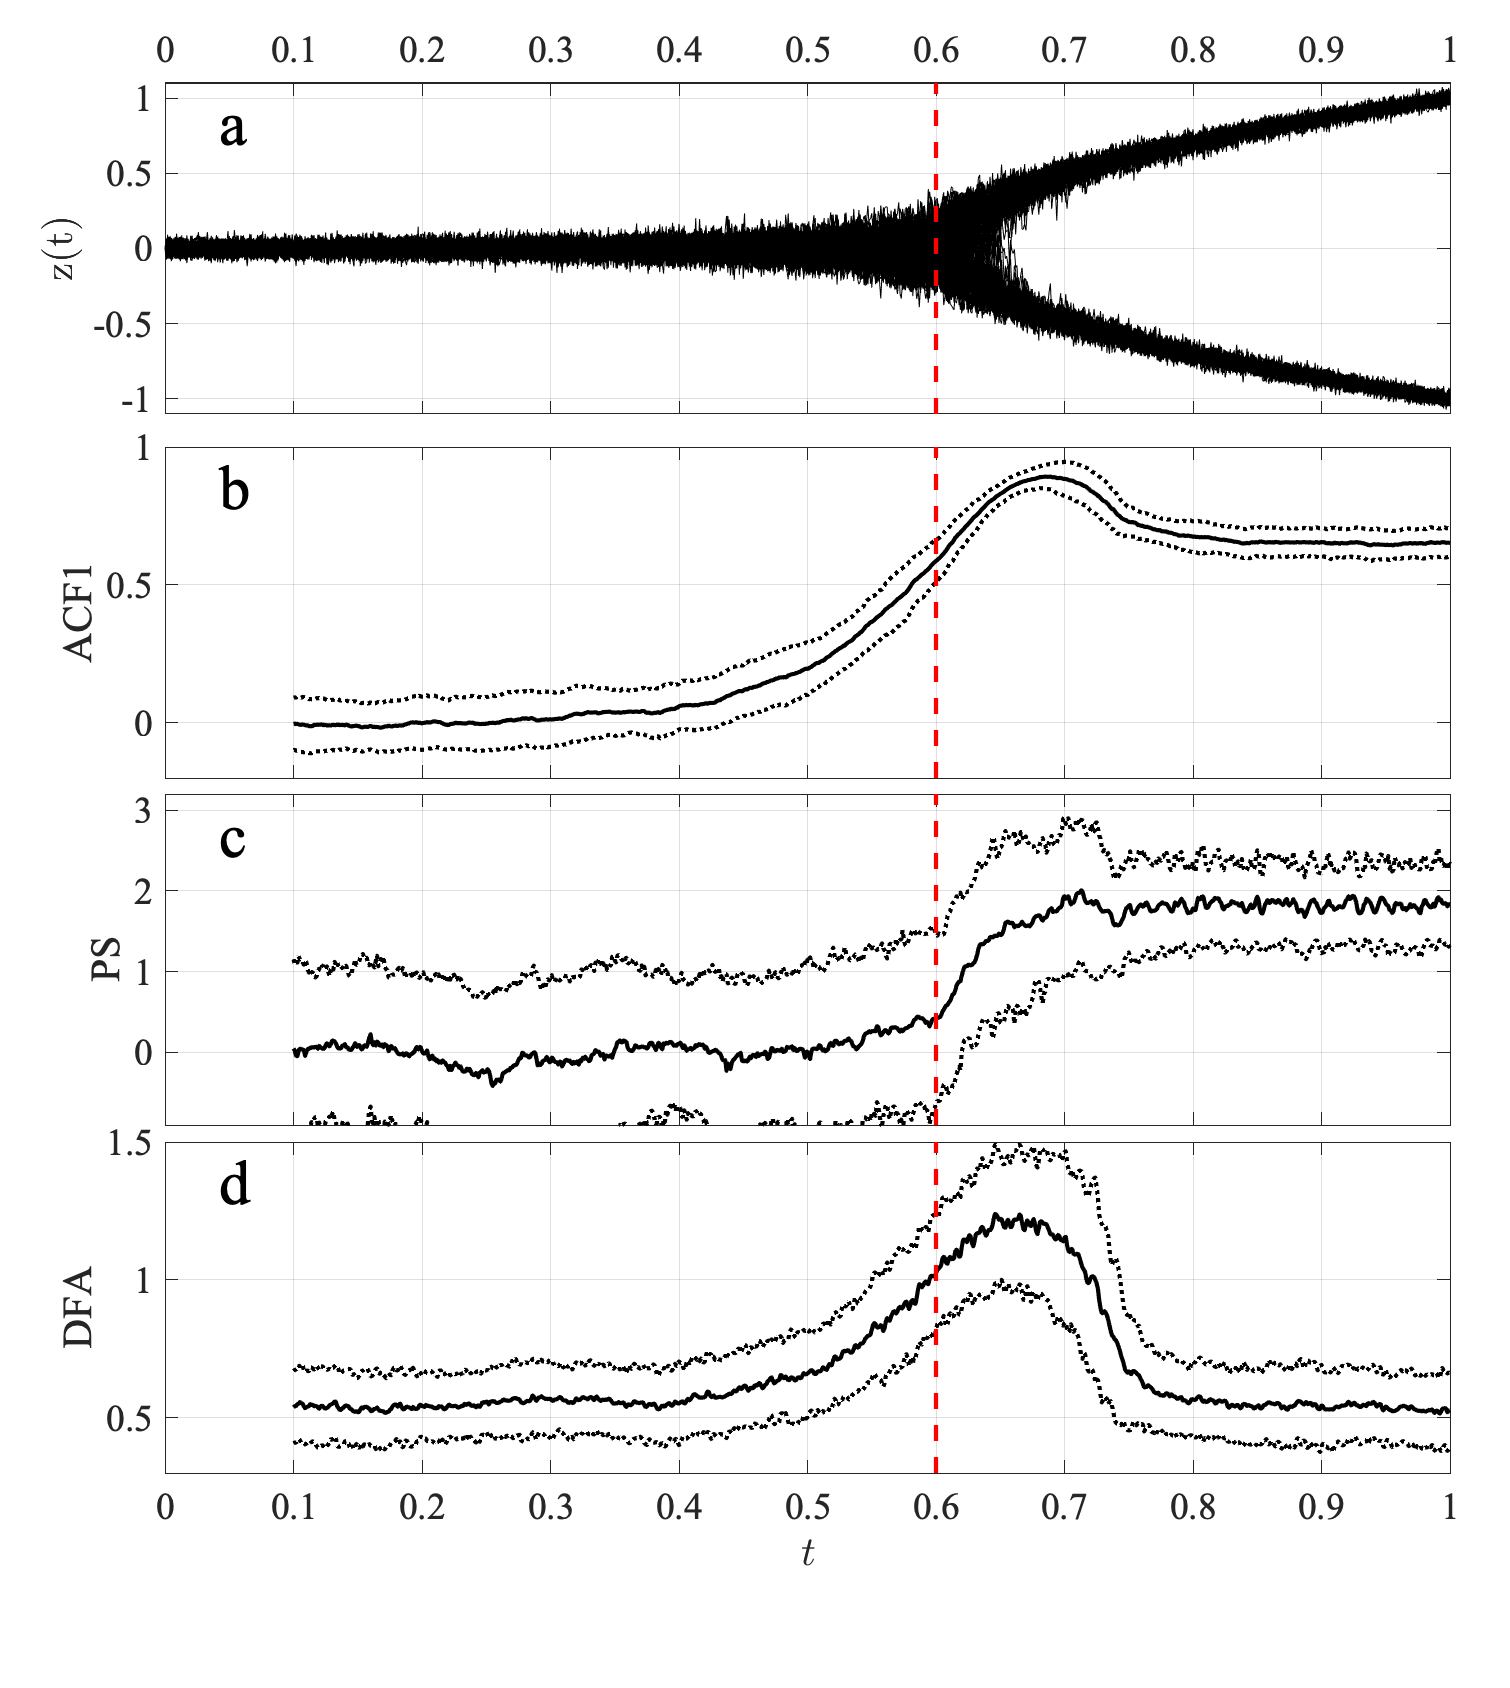
\includegraphics[width = 0.9\textwidth]{pitchforkEWS}
	\caption{\Red{ACF1, PS and DFA indicators applied to time series of the pitchfork bifurcation model. Panel {\bf a}: Data from an ensemble of $100$ runs of the model (see equation \ref{eqn:1D:EWS:Pitchfork}); Panels {\bf b}, {\bf c}, {\bf d}: The mean ACF1, PS and DFA indicators (all using window size 100) shown with error bars of one standard deviation.
	}}
	\label{fig:1D:pitchforkEWS}
\end{figure}

{\Red{Equation \ref{eqn:1D:EWS:Pitchfork} is integrated numerically with a time step of $\delta t =10^{\m5}$, from $t=0$ to $t=1$, and sampled at a rate of $10^3$ points per unit time to give a time series of length $N=10^3$. The ACF1, PS and DFA indicators are then applied with a window size of 100 points. This experiment is repeated for 100 such time series and the indicators are applied to all of them. The means of the indicator series are found and are plotted in figure~\ref{fig:1D:pitchforkEWS} with error bounds of one standard deviation.
		
We see that the ACF1 and DFA both provide an EWS, beginning to show a clear increasing trend at around $t=0.4$. The PS indicator, however, does not show a convincing trend (in the mean) until after the bifurcation has occurred, and the trend is not significant when the error bounds are taken into consideration. We do see that the PS indicator series shows a similar general shape to the ACF1 indicator: after increasing to a maximum value, both settle down to a constant value that is closer to that of red noise than white noise, whereas the DFA indicator settles back to a white-noise value ($0.5$ for DFA) after the bifurcation. The reason for the high value of the PS and ACF1 indicators after the bifurcation, although the system is trapped around a single stable point, much like before the bifurcation, is that the parabolic trend in the post-bifurcation system biases the autocorrelation whilst the detrending step in the DFA algorithm removes this and views both `single equilibrium' stages of the system equally. This is consistent with the findings presented in figure~\ref{fig:1D:PSsensitivity_trend} (page~\pageref{fig:1D:PSsensitivity_trend}), where both the PS and ACF1 indicators were biased by imposing a parabolic trend onto the AR(1) model when using a time series of $100$ points. Since the window size used for our experiment here was also $100$ points, we would expect the same result. For a window size of $10^5$ points we would expect (based on figure~\ref{fig:1D:PSsensitivity_trend}) that the PS indicator would not show bias. Given the highly variable performance of the PS indicator in that previous experiment, it is somewhat surprising that we any trend, even in the mean over an ensemble of $100$. 
}}


\begin{figure}
	\centering
	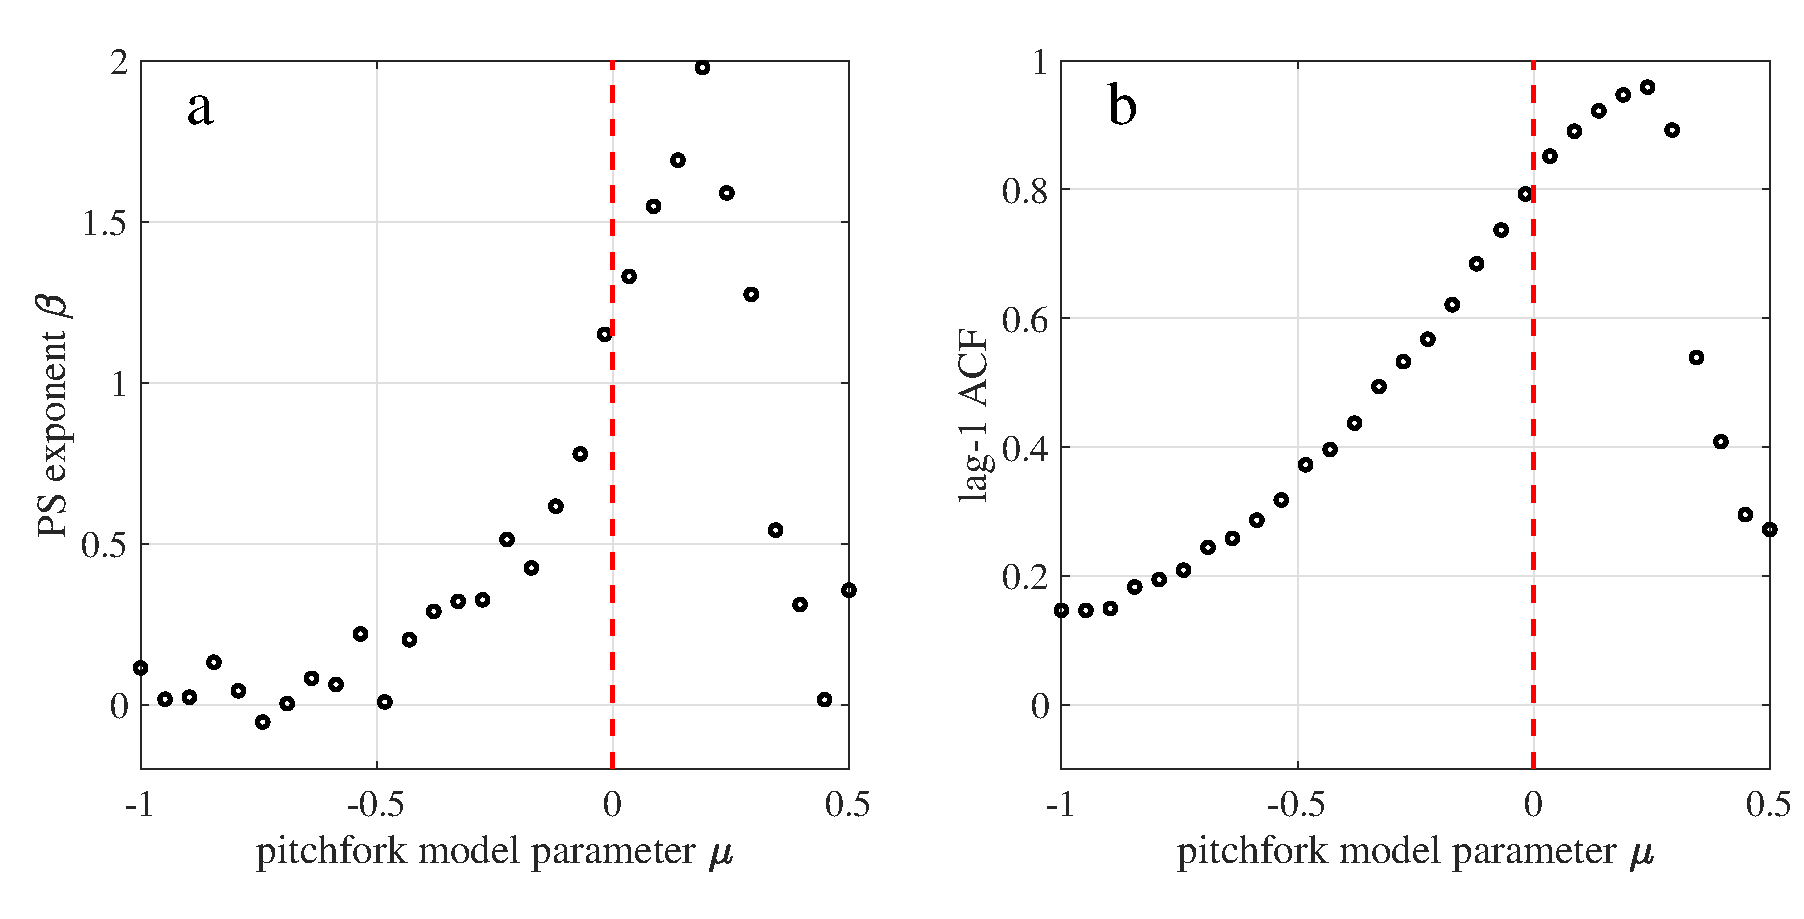
\includegraphics[width = 0.9\textwidth]{pitchforkMuRelationship}
	\caption{\Red{$30$ time series of length $10^5$ are created by integrating equation~\ref{eqn:1D:EWS:Pitchfork} using a \emph{constant} parameter $\mu$. Each time series uses a different constant value of $\mu$ between $\m1$ and $0.5$. The PS exponent (panel {\bf a}) and lag-1 autocorrelation (panel {\bf b}) are calculated for each time series.}}
	\label{fig:1D:pitchforkMuRelationship}
\end{figure}

{\Red{
		\subsubsection{Further experimentation}
		In order to further understand the relationship between the PS exponent and the parameter of the pitchfork model, we perform a more detailed experiment. In this case we use time series of length $10^5$, in order to see if significantly alters the results of the PS indicator, as was the case with the AR(1) model (see section~\ref{subsec:1D:Exponents_as_EWS:PSsensitivity}). 
		
		$30$ time series of length $10^5$ are created by integrating equation~\ref{eqn:1D:EWS:Pitchfork} using a \emph{constant} parameter $\mu$. Each time series uses a different constant value of $\mu$ between $\m1$ and $0.5$. The PS exponent and lag-1 autocorrelation are calculated for each time series. The results are shown in figure~\ref{fig:1D:pitchforkMuRelationship}. We see the same shape as in figure~\ref{fig:1D:pitchforkEWS}, with the values of the two indicators were plotted over time. Certainly the PS exponent are similarly related to the parameter of this pitchfork system just as they are for the AR(1) model, although there is much lower error involved in using the lag-1 ACF.
	}}

%\subsection{Early warning signals in the ??? system}
%\label{sec:1D:VanderPol}

%We now apply the 




\section{Discussion}
\label{sec:1D:discussion}

We have developed a novel indicator of EWS for tipping points in dynamical systems by estimating the power-law decay rate of the power spectrum in a sliding window \citep{prettyman2018}. {\Red{The PS exponent has been shown analytically to provide an indication of critical slowing down (see section~\ref{subsec:1D:Exponents_as_EWS:indicators}) based on the model of critical slowing down as an AR(1) process, and therefore the PS indicator is expected to provide an EWS of tipping points in the same way that the ACF1 and DFA indicators have previously been used.}} We have applied this PS indicator, along with the ACF1 and DFA indicators, to several different time series of models of various tipping points, including various bifurcations and non-bifurcational tipping. 

We have found that the PS indicator behaves similarly to the previously used ACF1 and DFA indicators applied to the model data, but with larger variance, which limits its usefulness in situations where the model has a noisy trajectory or cannot be observed multiple times.

Of the ACF, DFA and PS scaling exponents, all may be used as EWS indicators, although \citet{kantelhardt2001} notes that a direct calculation the ACF exponent $\gamma$ is often unsuitable and the DFA method is therefore introduced as an indirect measure. In our own implementations of the two methods, the ACF exponent is less reliable. The less computationally expensive lag-1 autocorrelation function is also often used instead of the ACF exponent since both provide a measure of critical slowing down (see equation \ref{eqn:1D:AR1_decay_model}), but it is highly sensitive to trends and periodicity. {\Red In contrast, the PS indicator is relatively insensitive to periodicity, as we have demonstrated in section~\ref{subsec:1D:Exponents_as_EWS:Periodicity} (page~\pageref{subsec:1D:Exponents_as_EWS:Periodicity}). The addition of a simple periodic function to an AR1 process does not affect the value of the PS exponent even whilst the lag-1 autocorrelation and DFA exponent are significantly affected so as to make the estimation of the model parameter (the critical slowing down proxy) impossible.}

\cite{heneghan2000} notes that the DFA and PS exponents have a predictable relationship and therefore the use of both is not necessary. {\Red{ However, this is true only when power-law scaling exists and does not hold when there is a cross-over in the power spectrum as demonstrated by the comparison in figure~\ref{fig:1D:ExponentRelationships}, nor may it be the case in oscillating systems. The choice between the two techniques may therefore be important when investigating tipping points, and the study of the behaviour of the PS exponent may reveal trends in the data which a study using the DFA or ACF exponents may not.}}
